\documentclass[11pt,a4paper,twoside]{article}
\usepackage[czech]{babel}
\usepackage[utf8]{inputenc}


%\usepackage[wordbk]{songbook} %bez akordů
\usepackage[chordbk]{songbook} %s akordy
\usepackage{multicol}
\setlength{\columnsep}{1.6cm}
\setlength{\columnseprule}{0.5pt}




\renewcommand{\ChFont}{\fontfamily{\sfdefault} \fontseries{bx}\fontshape{n}\fontsize{6mm}{0mm}\selectfont}




%%%%%%%%%%%%%%%%%
\makeatletter
\def\sbChord#1{%
  \ifx#1\relax%
    \let\next=\relax%
  \else%
    \ifx#1##% double sharp because we're inside a \def
      $\sharp$%
    \else%
      \ifx#1b%
        b% $\flat$ has been used in songbook, overwritting default behavious%
      \else%
        \ifx#1/%
          \ChBassFont /%
        \else%
          \ifx#1[%
            \bgroup\ChBkFont [\egroup%
          \else%
            \ifx#1]%
              \bgroup\ChBkFont ]\egroup%
            \else%
              #1%
            \fi%
          \fi%
        \fi%
      \fi%
    \fi%
    \let\next=\sbChord%
  \fi%
  \next%
}

\begingroup
  \lccode`\~=`\& % allow using & without \&
  \lowercase{\endgroup
    \def~{$\flat$}%
  }
\let\AKORD\Ch

\def\Ch{%
 % \begingroup
  \catcode`\&=\active
  \AKORD
}
\makeatother

%%%%%%%%%%%%%%%%%
\usepackage{suffix} %asterisk versions

\usepackage{enumitem,refcount}
\newcommand{\NADPIS}[1]{\section{#1}}
\newenvironment{TEXT}[1]
  {\NADPIS{#1}%
  \def\SLOKA{\item}
  \WithSuffix\newcommand\SLOKA*{\item[]}
  \def\REFREN{\item[Ref.:]}
  \def\REFRENHRAJ{}
  \def\INTERM{\item}
  \def\NL{\\*}
  \begin{enumerate}%
  }
  {\end{enumerate}}

%%%%%%%%%%%%%%%%%


%\usepackage[pdftex]{graphicx} % koliduje s watermarkem
%\usepackage{bookman}
%cislovani
%\usepackage{fancyhdr}
%\pagestyle{fancy}
%\fancyhf{} % smaže aktuální nastavení záhlaví a zápatí
%\fancyfoot[c]{\bfseries\thepage}                               % zrušení čísel stránek
%\renewcommand{\headrulewidth}{0pt} % tloušťka linky
%\renewcommand{\footrulewidth}{3pt}   % patička
%\addtolength{\headheight}{1.2pt}% prostor pro záhlaví
%\fancypagestyle{plain}{
%\fancyhead{} % na prázdných stránkách nechci záhlaví
%  \renewcommand{\headrulewidth}{0pt} % ani linku
%}
\usepackage[ddmmyyyy,hhmmss]{datetime}
\renewcommand{\dateseparator}{}
\renewcommand{\timeseparator}{}
\usepackage{tikz}

\usepackage{xcolor}

%\usepackage[printwatermark]{xwatermark}
%\newwatermark[evenpages,color=blue!20,angle=90,scale=5,xpos=90,ypos=-20]{D R A F T}
%\newwatermark[allpages,color=blue!20,scale=0.5,xpos=0,ypos=120]{\today\ \currenttime}
%\newwatermark[oddpages,color=blue!20,angle=90,scale=5,xpos=-80,ypos=-20]{D R A F T}


%%%%%%%%%%%%%%%%%%%%%%%%%%%
\usepackage{ulem}
\usepackage{amssymb}
\usepackage{mathtools}
\usepackage{mathabx}
\usepackage{wasysym}
\usepackage{fixltx2e}
%\usepackage{hyperref}
\newdimen\supsymwidth
\newdimen\supsymheight
\newdimen\tgtsymwidth
\setbox0=\hbox{$_\bigboxvoid$}
\supsymwidth=\wd0
\supsymheight=\ht0
\setbox0=\hbox{$_\bigovoid$}
\tgtsymwidth=\wd0

\newcommand{\supsym}[1]{%
%  \mathrlap{\bigboxvoid}
  \raisebox{-6pt}{\hbox to \supsymwidth{\hfill{\small#1}\hfill}}
}

%\newcommand{\target}[2][\relax]{$\supsym{#1}$\uline{#2}}
\newcommand{\VOLTA}[2][\relax]{\textsubscript{\small#1}\uline{#2}}
%%%%%%%%%%%%%%%%%%%%%%%%%%%

\usepackage{ifthen}

\newcommand{\newevenside}{
	\ifthenelse{\isodd{\thepage}}{\newpage}{
	\newpage
        \phantom{placeholder} % doesn't appear on page
	\thispagestyle{empty} % if want no header/footer
	\newpage
	}
}
%
%
%  nastavení sekcí a jejich stránkování
%\usepackage{sectsty}
%\sectionfont{\Huge}
\usepackage{titlesec}
\usepackage{needspace}
\titleformat{\section}
{\needspace{5cm}\Huge\bfseries}{}{1ex}{\thesection ~}

%\let\stdsection\section
%\renewcommand\section{\ifthenelse{\isodd{\thepage}}{\newpage}{}\stdsection}


\footskip 0cm
\unitlength 1mm

\topmargin 0.5cm
\headheight 0cm
\headsep 20pt
\textheight 27.5cm
\textwidth 16cm   %přesáhne maximálně 0.5 cm za okraj   (59 Ví Bůh kolik...)
\marginparsep 1cm
\marginparwidth 0cm

\oddsidemargin 4cm
\evensidemargin 1cm


\pagestyle{empty}



\usepackage[export]{adjustbox}


%--------------------------------------nastavení obsahu
\newlength\widest
\settowidth\widest{990.99.}
\usepackage[]{titletoc}
\titlecontents{section}[1pc]
{\addvspace{0pc}}
{\parbox[t]{\widest}{\hfill\thecontentslabel}
\hspace{3mm}}
{}
{}
[\addvspace{0pt}]
%-------------------------------------------------



%\usepackage{fullpage}
\leftskip=0cm
%\usepackage{sectsty}
%\allsectionsfont{\usefont{OT1}{phv}{bc}{n}\fontsize{28}{1}\selectfont}


%\newcommand\uv[1]{\quotedblbase #1\textquotedblleft}%
\setlength{\parindent}{0cm}



%opening

\title{TÁBOROVÝ ZPĚVNÍK}
\author{ROSOMÁK}

\begin{document}

\sffamily
\huge

%\begin{titlepage}

%\begin{center}

%\parbox{14cm}
%\ \vfil
\vspace*{2mm}
\hspace*{-0.15\textwidth}
\begin{tikzpicture}[remember picture,overlay]
\node at (165mm,-1.5mm) {\tiny ver.\yyyymmdddate\today\currenttime};
\end{tikzpicture}
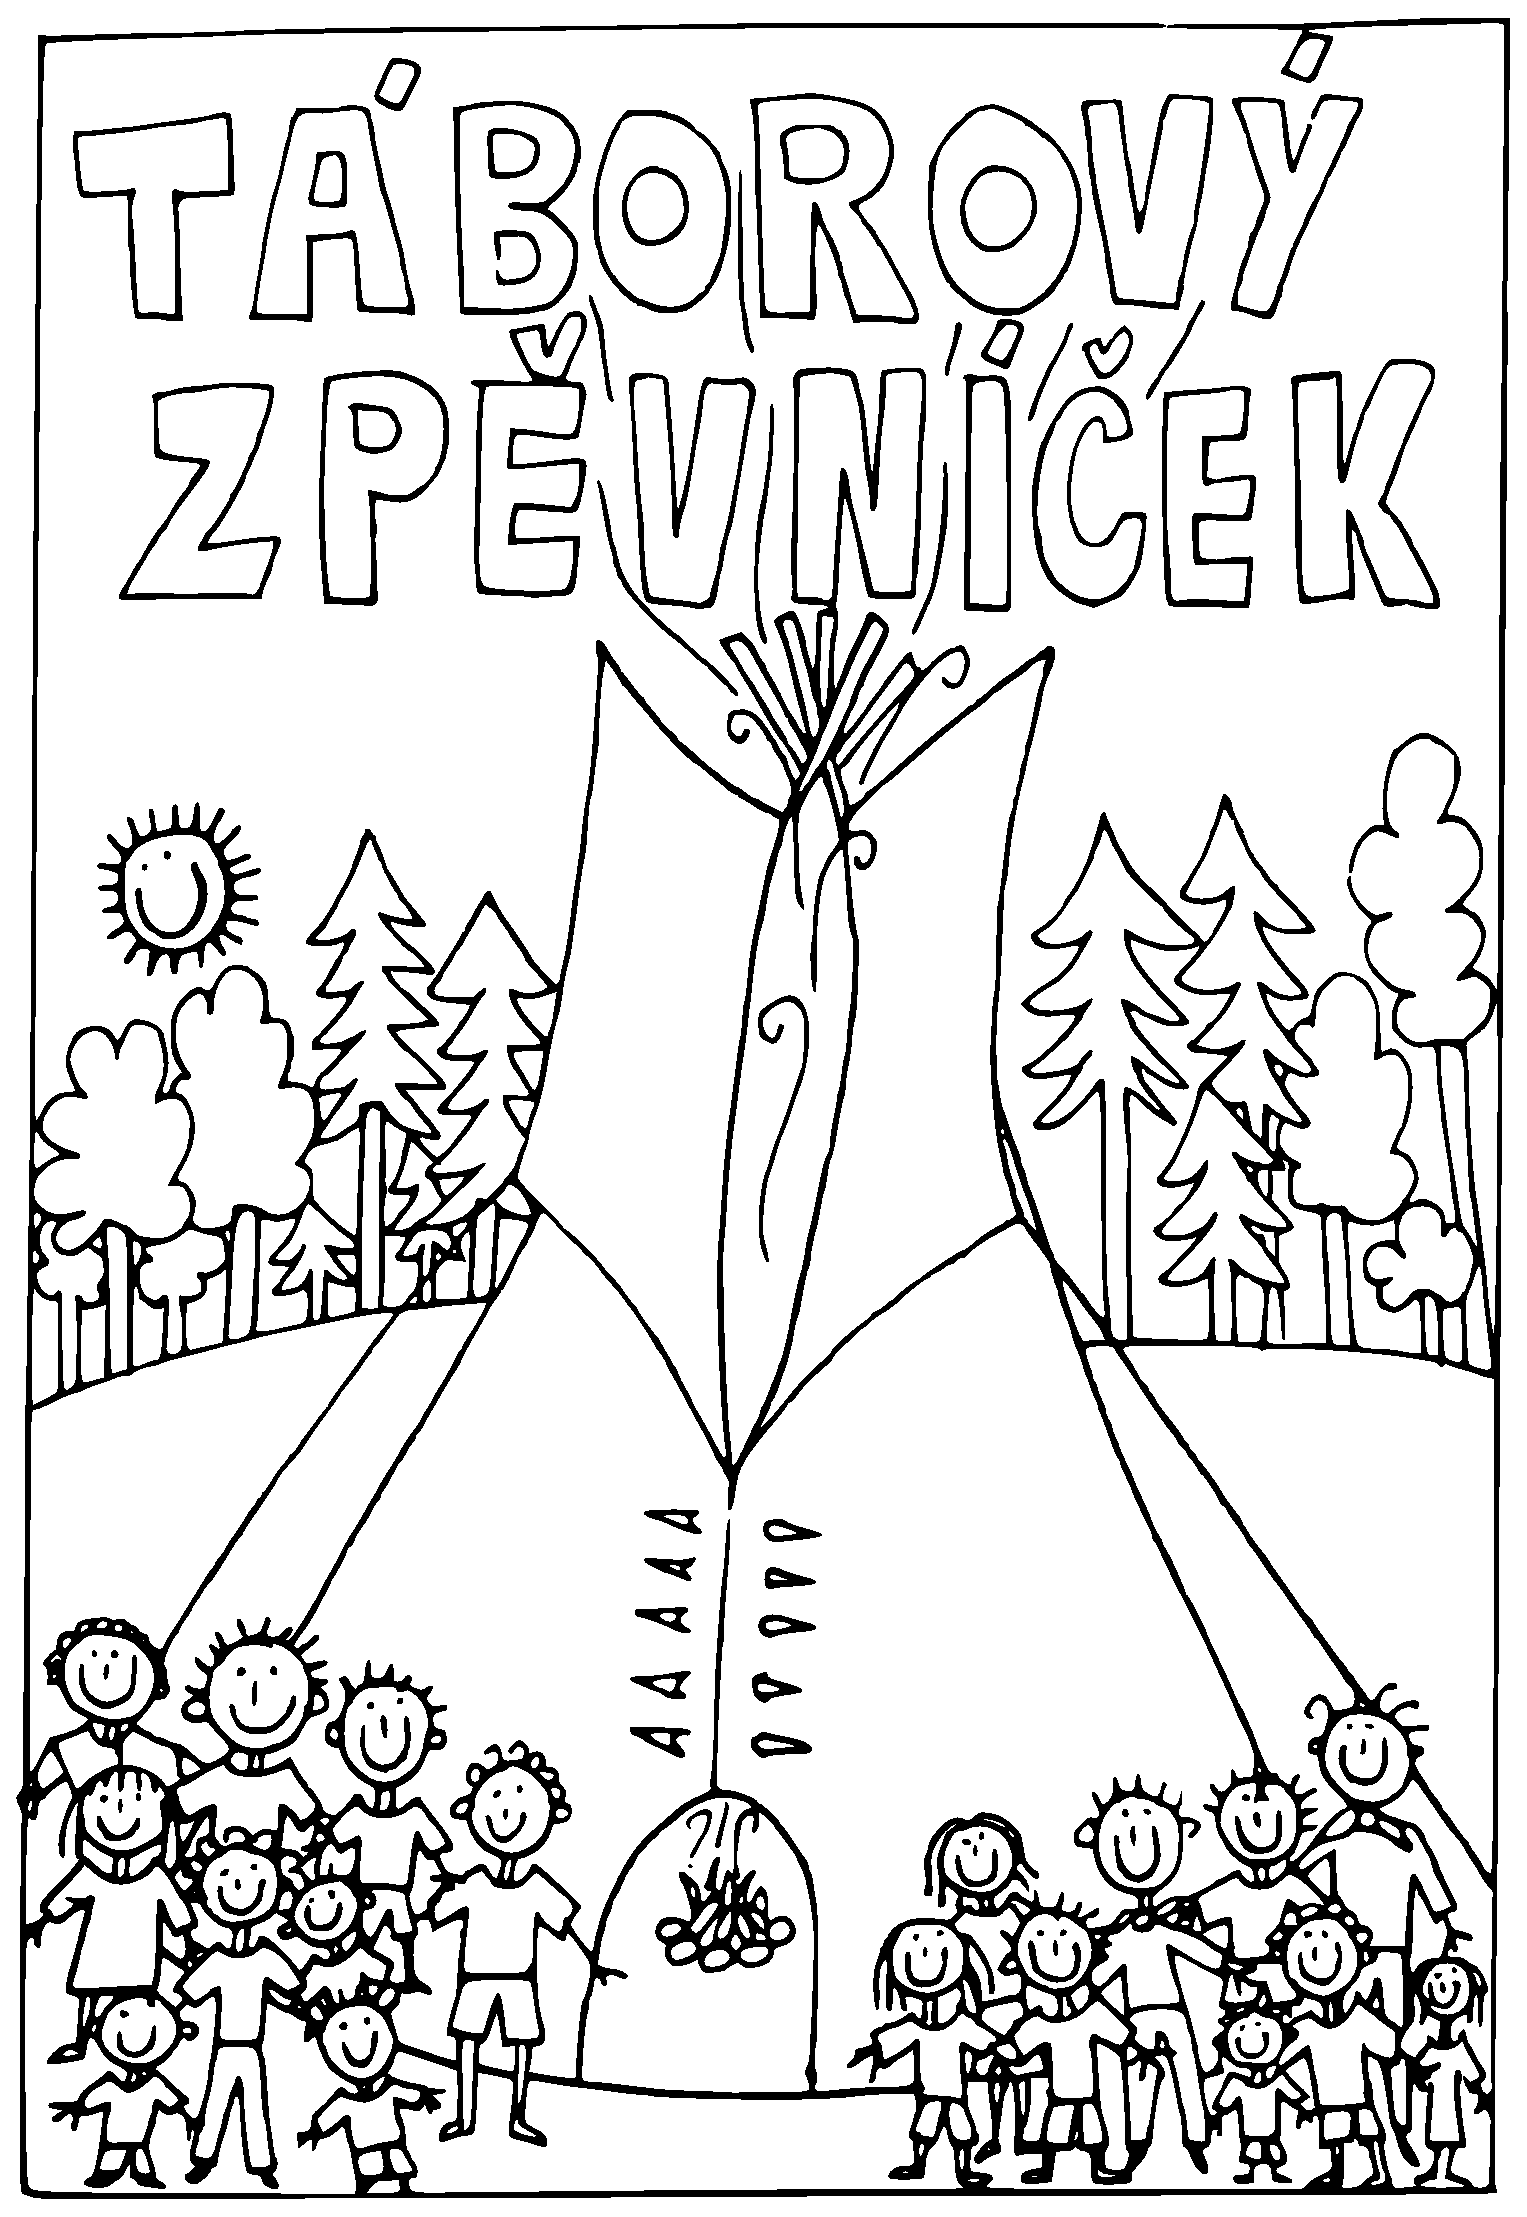
\includegraphics[width=1.05\textwidth]{images/titulni.eps}
\vfil\

%\end{titlepage}

\vspace*{3cm}
\parbox{14cm}{\centering \huge \itshape \bfseries Pane slyš náš hlas \\*
chcem' tě chválit zas \\*
za to že máš v péči\\*
celý svět i nás}
\vspace*{15cm}
%\\*\line(1,0){450}
\\*
\parbox{14cm}{\centering Vydalo sdružení YMCA -- Jindřichův Hradec \\*
pro potřeby letních táborů, \the\year \\*
NEPRODEJNÉ\,!}

\section{Apoštolská}
\begin{enumerate}
\item \Ch{C}{Prosíme} tě \Ch{G}{dej} nám Pane \Ch{a}{sílu} \Ch{C7}{ }\\*
\Ch{F}{chceme} začít \Ch{f}{podle} slov tvých \Ch{d(7)}{žít} \Ch{G}{ } \\*
\Ch{C}{věříme}, že \Ch{E7}{jednou} budem \Ch{a}{v míru} \\*
\Ch{C7}{společně} u \Ch{F}{tvého} stolu \Ch{G}{víno} \Ch{C}{pít} \Ch{(G)}{ }  
\item Dívej se na všechny naše zkoušky \\*
jak se utápíme v starostech \\*
Bez tebe by svět byl jenom pouští \\*
bez tebe by život neměl vůbec žádný cíl 
\item = 1. \\*
\end{enumerate}
 % 1
\pagebreak
\section{Bojujte dál}
\begin{enumerate}
\item[Ref.:]  \Ch{D}{Bojujte} \Ch{G}{bojujte} d\Ch{D}{ál} \\*
\Ch{D}{Bojujte} \Ch{E7}{bojujte} d\Ch{A7}{ál} \\*
\Ch{D}{ }pohleďte \Ch{D7}{jen} \Ch{G7}{v dálce} svítá \\*
\Ch{D}{ }pohleďte \Ch{D7}{je}n \Ch{G7}{den} nás vítá \\*
\Ch{D}{bojujte} \Ch{G}{bojujte} d\Ch{D}{ál} 
\item \Ch{D}{Zpříma} choďte \Ch{f#}{pozdvihněte} hlavu \Ch{D7}{ } \\*
\Ch{G}{i když} pro vás vavřín neros\Ch{D}{te} \Ch{G7}{}\\*
\Ch{D}{nechte} mocným \Ch{f#}{moc} a slavným \Ch{D7}{slávu} \\*
\Ch{E7}{o jejich} se přízeň nepros\Ch{A7}{te} 
\item Kdo se ani zlatem koupit nedá \\*
nemlčí a s proudem nepluje \\*
spravedlnost kdo ve světě hledá \\*
v jedné řadě s námi bojuje 
\item K útěku-li z boje chytrost radí \\*
holubičí mějte prostotu \\*
opatrní buďte jako hadi \\*
nezběhněte z cesty k životu 
\item Bojujte však pomstu nechte Pánu \\*
On je soudce a sám určí trest \\*
Prohraje kdo ranou splácí ránu \\*
k nenávisti kdo se nechá svést \pagebreak
\item Neusněte ať vejdete zítra \\*
v zemi novou v zaslíbenou vlast \\*
Nocí ať vás vede příslib jitra \\*
vládou temna nenechte se zmást 
\end{enumerate}
 % 2
\section{Čest dej}
\begin{enumerate}
\item[Ref.:] /: \Ch{E(E,A,E)}{Čest dej, jen Pánu Bohu svému dej} :/                      4x \\*
  P\Ch{E}{án} jen, Pán jen,\Ch{A}{ jen }Pán buď \Ch{F#}{oslaven} \\*             %\Ch{f\#$}
P\Ch{E}{án} jen \Ch{A}{Pán} buď osla\Ch{E}{ven} 
\item \Ch{E}{Přijde} k tobě ďábel sám, \Ch{A}{abys} před ním \Ch{E}{klek'} \\*
na to dobrou \Ch{c#}{radu} mám, \Ch{F#}{vyzkoušený} \Ch{H7}{lék} \\*
\Ch{E}{Moc} i slávu, \Ch{E7}{světa} říš \Ch{A}{vše} ti nabí\Ch{Edim}{dne} \\*
\Ch{E}{ty} mu na to \Ch{c#}{odpovíš:} \Ch{F#}{ne,} \Ch{H7}{ne,} \Ch{E}{ne} 
\item Bez fára a bez vily nemáš úroveň \\*
co tě v mládí učili na to zapomeň \\*
celý svět už věří teď jen v to tele zlacené \\*
Dáš jim na to odpověď: ne, ne, ne 
\item Všední den se promění v cestu do ráje \\*
marjánkový koření věc moc dobrá je \\*
strach a smutek šeď a tíž z tebe opadne \\*
Ty jim na to odpovíš: ne, ne, ne 
\item Kočku chtěla sežrat myš, dvakrát dvě je pět \\*
tak nám to tu podepiš, otevřeš si svět \\*
však jsou slova jak sám víš proutky čarovné \\*
Ty jim na to odpovíš: ne, ne, ne \\*
\end{enumerate}
 % 3
\begin{TEXT}{Dál přece nejdeme sami}
\SLOKA \hspace{0em}\rlap{\Ch{C}{Dál} přece nejdeme sami} \hspace*{0.6\textwidth}\rlap{\Ch{D}{ }}\NL
\hspace{0em}\rlap{\Ch{G7}{dál} Pán tu zůstává s námi} \hspace*{0.6\textwidth}\rlap{\Ch{A7}{ }}\NL
\hspace{0em}\rlap{\Ch{C}{dál} cestu určil svým dětem} \hspace*{0.6\textwidth}\rlap{\Ch{D}{ }}\NL
\hspace{0em}\rlap{\Ch{G}{dál} tímto \Ch{C}{světem} -- \Ch{G}{ha}\Ch{C}{le}\Ch{F}{lu}\Ch{C}{ja} \Ch{G7}{ } } \hspace*{0.6\textwidth}\rlap{\Ch{A\ \ D\ \  A\ D\ G\ D\ A7}{ }}
\SLOKA S ním cesta není tak těžká \NL
s ním každá chvíle je hezká \NL
s ním jdeme všichni a spolu \NL
s ním jdeme domů -- haleluja 
\end{TEXT}

 % 4
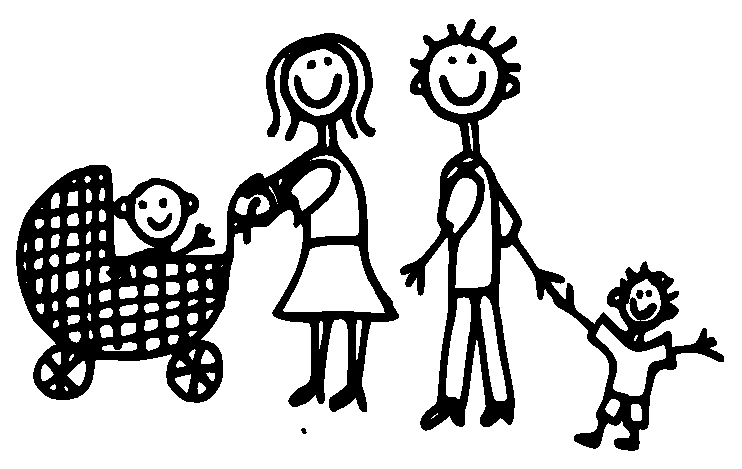
\includegraphics[width=8cm]{images/1.eps}
%\vfil
\begin{TEXT}{Děkujem Ti Pane Bože}
\SLOKA \Ch{C}{Dě}ku\Ch{a}{jem} Ti \Ch{d}{Pa}ne \Ch{G}{Bože} \Ch{C}{že} nás \Ch{F}{máš} tak \Ch{G}{rád}\NL
\Ch{e}{že} jsme \Ch{a}{moh}\Ch{F}{li} \Ch{C}{dneska} \Ch{G}{ráno} \Ch{a}{zdra}\Ch{G}{ví} \Ch{C}{vstát} \Ch{G}{ } \Ch{C}{ } 
\SLOKA Děkujem Ti Pane Bože že si smíme hrát \NL
že si také můžem spolu zazpívat 
\SLOKA Děkujem Ti Pane Bože za ten dnešní den \NL
dej ať tebe každý chválí v srdci svém \NL
\end{TEXT}
 % 5
%\pagebreak
\begin{TEXT}{De profundis}
\SLOKA \Ch{e}{Temnou,} divnou \Ch{h}{mlhou} bloudím \Ch{C}{sem} a tam \Ch{Cmaj7}{ }\NL
\Ch{a}{černá} s bílou \Ch{h}{smíchaly} se \Ch{e}{spolu} \Ch{h}{ } \NL
\Ch{e}{Nevidím} už, \Ch{h}{co} je pravda, \Ch{C}{co} je klam \Ch{Cmaj7}{ } \NL
\Ch{a}{nevím,} jdu-li \Ch{h}{nahoru}, či \Ch{e}{dolů }\Ch{h}{ }
\REFREN  \Ch{e}{Řekni} slovo, řekni slovo, Pane\NL
\Ch{A}{ať} pomine tahle šedá tma\NL
\Ch{C}{řekni} slovo a zázrak se stane \NL
uzdra\Ch{G}{vena} \Ch{a}{bude} \Ch{h}{duše} \Ch{e(E)}{má }
\SLOKA Nerozeznám dobře okraj propasti\NL
nevím, je-li na krok dosti místa\NL
Strach mám, abych neupadl do pasti\NL
kterou na mne pokušení chystá
\SLOKA Přízrak noční sleduje mne potají\NL
divné hlasy otázku mi kladou\NL
divné hlasy otázku mi šeptají\NL
k čemu věrnost, nač pohrdat zradou\NL
\end{TEXT}
 % 6
\begin{TEXT}{Díky}
\SLOKA \Ch{D}{Díky} \Ch{h}{za} toto \Ch{e}{krásné} \Ch{A7}{ráno} \NL
\Ch{D}{díky} \Ch{h}{za} každý \Ch{e}{nový} \Ch{A7}{den} \NL
\Ch{D}{díky} \Ch{D7}{ za to}, co \Ch{G}{už} je \Ch{g}{za} mnou \NL
\Ch{D}{ja}\Ch{(h)}{ko} \Ch{e}{těž}\Ch{A}{ký} \Ch{D}{sen} \Ch{(A7)}{ }  
\SLOKA \Ch{D}{Díky} \Ch{h}{za} všechny \Ch{e}{věrné} \Ch{A7}{druhy} \NL
\Ch{D}{díky} \Ch{h}{ó} Pane \Ch{e}{za} tvůj \Ch{A7}{lid} \NL
\Ch{D}{díky} \Ch{D7}{že} všechny \Ch{G}{křivdy} \Ch{g}{dluhy} \NL
\Ch{D}{mo}\Ch{(h)}{hu} \Ch{e}{od}\Ch{A}{pus}\Ch{D}{tit} \Ch{(H7)}{ } 
\SLOKA \Ch{E}{Díky} \Ch{c#}{za} moje \Ch{f#}{pra}co\Ch{H7}{viště} \NL
\Ch{E}{díky} \Ch{c#}{za} každý \Ch{f#}{drobný} \Ch{H7}{zdar} \NL
\Ch{E}{díky} \Ch{E7}{za} všechno \Ch{A}{krásné} \Ch{a}{čisté} \NL
\Ch{E}{dík} \Ch{(c#)}{za} \Ch{f#}{hud}\Ch{H7}{by} \Ch{E}{dar} \Ch{(H7)}{ } 
\SLOKA \Ch{E}{Díky} \Ch{c#}{za} to co \Ch{f#}{zar}mou\Ch{H7}{tilo} \NL
\Ch{E}{díky} \Ch{c#}{za} to co \Ch{f#}{potě}\Ch{H7}{ší} \NL
\Ch{E}{díky} \Ch{E7}{že} vedeš \Ch{A}{mne} má \Ch{a}{sílo} \NL
\Ch{E}{ces}\Ch{(c#)}{tou} \Ch{f#}{nej}\Ch{H7}{lep}\Ch{E}{ší} \Ch{(C7)}{ } \pagebreak
\SLOKA \Ch{F}{Díky} \Ch{d}{že} smím tvé \Ch{g}{Slovo} \Ch{C7}{chválit} \NL
\Ch{F}{díky} \Ch{d}{že} Ducha \Ch{g}{dáš} mi \Ch{C7}{též} \NL
\Ch{F}{díky} \Ch{F7}{že} nablíz\Ch{B}{ku} i v \Ch{b}{dá}li \NL
\Ch{F}{li}\Ch{(d)}{di} \Ch{g}{mi}\Ch{C7}{lu}\Ch{F}{ješ} \Ch{(D7)}{ }
\SLOKA \Ch{G}{Díky} \Ch{e}{že} všem jsi \Ch{a}{přines} \Ch{D7}{spásu} \NL
\Ch{G}{díky} \Ch{e}{toho} se \Ch{a}{přidr}\Ch{D7}{žím} \NL
/: \Ch{G}{díky} \Ch{G7}{že} věřím \Ch{C}{tvé}mu \Ch{c}{hlasu} \NL
\Ch{G}{že} \Ch{(e)}{ti} \Ch{a}{pat}\Ch{D7}{řit} \Ch{G}{smím} :/ \NL
\end{TEXT}
 % 7
\vfil
\section{Do tvých starostí}         % akordy z NETU
\begin{enumerate}
\item[A.] \Ch{D}{Do} tvých staros\Ch{A}{tí} \Ch{h}{smutků} úzkos\Ch{f#}{tí } \\*
\Ch{G}{přišel} ten, kdo \Ch{D}{má} tě \Ch{h}{rád} a \Ch{e}{z bíd} tě \Ch{A}{vy}pros\Ch{D}{tí} 
\item[B.] Králů Král, pánů Pán \\*
je nám bez rozdílu všechněm zvěstován \\*
\end{enumerate}
 % 8
\pagebreak
\section{Doufej v Hospodina}  % zpěvník Laudate
\begin{enumerate}
\item[A.] \Ch{D}{Doufej} v Hospodina \Ch{G}{celým} srdcem svým \\*
a \Ch{D}{na} rozumnost svou se \Ch{A}{nespoléhej} \\*
\Ch{D}{Na} všech cestách svých snaž \Ch{G}{se} jej poznávat \\*
On \Ch{D}{spravovati} \Ch{A}{bude} cesty \Ch{D}{ }své
\item[B.] Doufej v Boha, Hospodina \\*
doufej v Pána, on spravovati bude stezky tvé.
\end{enumerate}
 % 9
%\vfil
\begin{TEXT}{Duha}
\SLOKA Stará \Ch{C}{archa} \Ch{G}{chrání} Noa \Ch{E7}{před} vo\Ch{A7}{dou} \NL
\Ch{D7}{Bůh} duhu \Ch{G7}{na} oblohu \Ch{C}{dá} \Ch{(G)}{ } \NL
bouře \Ch{C}{valí }\Ch{G}{se} pod temnou \Ch{E7}{oblo}\Ch{A7}{hou} \NL
\Ch{F7maj}{Bůh} duhu \Ch{G7}{na} oblohu \Ch{C}{dá} 
\REFREN  /: \Ch{C(F)}{Když černej} \Ch{G(E7)}{mrak na} nebi \Ch{C(a)}{slunce zakrej}\Ch{C7(G)}{vá :/} \NL
navzdo\Ch{C}{ry} černej \Ch{B}{tmám} duha \Ch{A7}{nám} jak slunce \Ch{D7}{svítí} \NL
\Ch{F7}{Bůh} duhu \Ch{A&7}{na }ob\Ch{G7}{lohu} \Ch{C}{dá} \Ch{G}{}
\SLOKA Jít se dá i poušti sluncem spálené, Bůh… \NL
kdo jde za ní dojde k zemi slíbené, Bůh… 
\SLOKA Kalný Jordán přejít brání dravý proud, Bůh… \NL
kdo jde za ní ten nemůže utonout, Bůh… \NL
\end{TEXT}
 % 10
\pagebreak
\section{Het bot ba}
\begin{enumerate} 
\item \hspace{0em}\rlap{/: \Ch{C7}{Het} bót \Ch{F}{ba} to \Ch{C}{ba'a} ba \Ch{F}{kot}ba i joi \Ch{d}{jem} } \hspace*{0.75\textwidth}\rlap{\Ch{D7\,G\,D\,G\,e}{ }}\\*
\hspace{0em}\rlap{me \Ch{g}{ga} bal \Ch{B}{lón}\Ch{C}{ni} \Ch{F}{bo} :/ } \hspace*{0.75\textwidth}\rlap{\Ch{a\,C\,D\,G}{ }}\\*
\hspace{0em}\rlap{/: Bal lonni \Ch{C7,F}{bo :/} } \hspace*{0.75\textwidth}\rlap{\Ch{D7,G}{ }}\\*
Het bot ba… 
\item /: Kde se dva neb tři ve jménu mém sejdou \\*
já uprostřed nich jsem :/ \\*
/: Uprostřed jsem :/ \\*
Kde se dva neb tři…
\item = 1.
\end{enumerate}
 % 11
\vfil
\begin{TEXT}{Hosana}
\SLOKA /: Ho\Ch{G}{sana}, ho\Ch{D}{sana}, ho\Ch{e}{sana} Bohu \Ch{C}{na} ne\Ch{D}{bi} :/ \NL
\Ch{C}{ }Jméno \Ch{D}{slavíme} tv\Ch{G}{é} \Ch{C}{  }chválí \Ch{D}{tě} srdce m\Ch{G}{é } \NL
\Ch{C}{ } Vyvý\Ch{D}{šen} buď ó \Ch{G}{Bo}\Ch{D}{že} \Ch{e}{náš}, ho\Ch{C}{sana} Bohu \Ch{D}{na} ne\Ch{G}{bi.} 
\SLOKA /: Sláva, sláva, sláva všech králů Králi :/ \NL
Jméno slavíme tvé… \NL
… sláva tobě Králi náš. 
\SLOKA = 1. \NL
\end{TEXT}
 % 12
\begin{TEXT}{Hříchy}
\REFREN  Hříchy \Ch{a}{tvý} tě \Ch{F}{jednou} \Ch{G}{do}že\Ch{a}{nou} \NL
zkoušíš spálit \Ch{G}{mosty} za se\Ch{C}{bo}\Ch{a}{u} \NL
všechno zlý v duší \Ch{a7}{dál} si \Ch{G}{vlá}\Ch{F}{číš} \Ch{a}{tmou} \NL
hříchy tvý tě \Ch{F}{jednou} \Ch{G}{do}že\Ch{a}{nou} 
\SLOKA \Ch{a}{Váháš} jestli \Ch{G}{má} cenu se \Ch{C}{prá}\Ch{a}{t} \NL
váháš jestli \Ch{G}{znova} začít \Ch{C}{hrá}\Ch{a}{t} \NL
hříchů svých snad \Ch{F}{začít} \Ch{G}{lito}\Ch{a}{vat} 
\SLOKA Troufám si ti dát to oč jsi stál \NL
troufám si tě vést zas o krok dál \NL
/: Hříchy tvý na sebe jeden vzal :/ \NL
\end{TEXT}
 % 13
\vfil
\section{Hvězda}
\begin{enumerate}
\item \Ch{C}{ }Tomu, kdo \Ch{a7}{pro} žal hlavu \Ch{d7}{věší,} \\*
\Ch{G}{ } na nebi hvězda \Ch{Cmaj}{září,} \\*
\Ch{Fmaj}{zahání} tmu a smutné \Ch{d}{těší,} \\*
\Ch{G}{ } osuší slzy z \Ch{C}{tváří}.
\item Sníh na dlani tě bude hřát\\*
a mráz ten nespálí tě,\\*
vlk s beránkem si bude hrát\\*
a králem bude Dítě.\\*
\end{enumerate}
 % 14
\section{Hvězdy tiše vyšly}
\begin{enumerate}
\item \Ch{D}{Hvězdy} tiše vyšly \Ch{e}{kuřátka} šla \Ch{A}{spát} \\*
\Ch{D}{v ochra}\Ch{f#}{nu} tvou \Ch{h}{Bo}\Ch{G}{že} \Ch{D}{chci} se \Ch{A7}{odevz}\Ch{D}{dat} 
\item Děkuji i prosím za dar života \\*
za vše co mi dává tvoje dobrota 
\item Opatruj mi všechny které mám tak rád \\*
uč mne mluvit pravdu lži se vystříhat 
\item Buď tak jako ve dne v noci se mnou zas \\*
k práci včas mne probuď opět v jitřní čas \\*
\end{enumerate}
 % 15
\vfil
\section{Chci Pane chválit tě}            % akordy z NETU
\begin{enumerate}
\item[Ref.:]   /: Chci Pane \Ch{E(c#)}{chválit tě} den ode dne víc :/ \\*
\Ch{A}{hle}dat tvoji tvář po\Ch{f#}{znávat} milost tvou \\*
chci tebe \Ch{E}{chvá}\Ch{H}{lit} 
\item Chci tebe více znát… 
\item Chci     k tobě lásku mít… 
\item Jen tobě sloužit chci…
\item[] (Druhý hlas: Ptáci v oblacích tobě zpívají, \\*
stromy na polích ruce zvedají, \\*
i já zpívat chci, ruce pozvednout k oslavě tvé.) \\*
\end{enumerate}
 % 16
\vfil
\hspace*{1cm}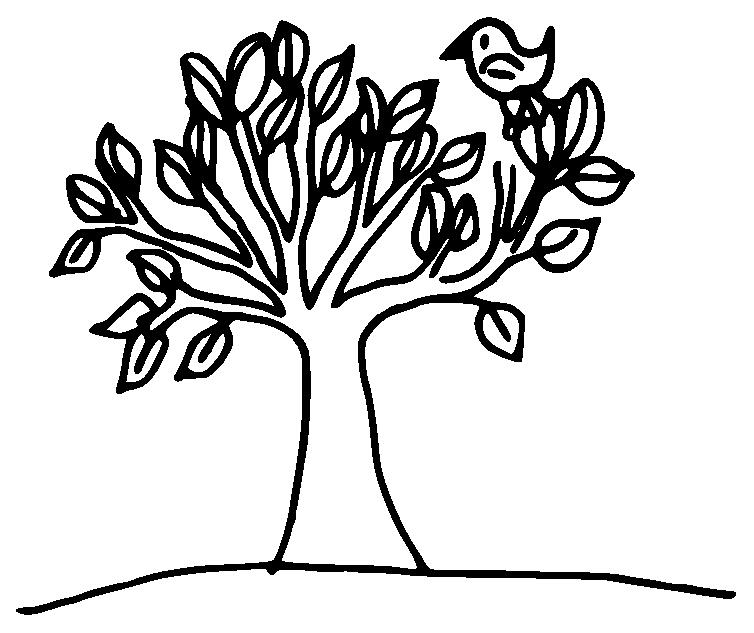
\includegraphics[width=12cm]{images/2.eps}
\vfil
\begin{TEXT}{Chvalozpěv}
\SLOKA \Ch{G}{Neskládejte} \Ch{a}{v mocných} nadě\Ch{D}{ji} \NL
\Ch{a}{v síle} jejich, \Ch{h}{která} skály \Ch{e}{lá}\Ch{a}{me} \Ch{e}{ } \Ch{D7}{ } \NL
\Ch{G}{ochabne} dřív \Ch{a}{nebo} pozdě\Ch{D}{ji} \NL
\Ch{a}{nedoufejte} \Ch{h}{v zdání} které \Ch{e}{klame} \Ch{A}{ } 
\REFREN  \Ch{D}{Ty} jsi hoden \Ch{G}{žehnání} a \Ch{D}{chvály} \Ch{G}{ } \NL
\Ch{D}{tvoji} moc a \Ch{G}{sílu} slaví\Ch{D}{me} \Ch{G}{ } \NL
/:\Ch{D}{ }před tebou se \Ch{e}{Pane} Kriste \Ch{f#}{králů} \Ch{G}{Králi} \NL
\Ch{e}{dobrovolně} \Ch{A7}{sklání}\Ch{D}{me}  :/
\SLOKA Vláda jeho není na chvíli \NL
pravda věčná platí v jeho říši \NL
v jeho panství není násilí \NL
blaze tomu kdo hlas jeho slyší 
\SLOKA Žíznivým dá napít z pramene \NL
nedolomí nalomenou třtinu \NL
proměňuje srdce kamenné \NL
odpustí i zbloudilému synu 
\SLOKA Znaveným on síly dodává \NL
uvězněným snímá pouta z rukou \NL
stojí při těch kdo jsou bez práva \NL
otevírá všechněm kteří tlukou \NL
\end{TEXT}
 % 17
\section{Jak dobré a utěšené}
\begin{enumerate}
\item /: \Ch{d}{Jak} dobré a utě\Ch{g}{še}\Ch{d}{né} \Ch{a}{žijí-li} bratři \Ch{d}{v lásce} :/ \\*
/: \Ch{d}{Radost} \Ch{g}{ma}\Ch{d}{jí} \Ch{a}{v lásce} když přebý\Ch{d}{vají} :/ 
\item … sestry… 
\item … všichni… 
\end{enumerate}
 % 18
\pagebreak
\begin{TEXT}{Jednou přijde smrtka}
\SLOKA \Ch{G}{Je}dnou přijde \Ch{C}{smrtka} s \Ch{G}{ko}sou \Ch{C}{ }\NL
\Ch{G}{žlu}té tělo \Ch{C}{bu}de na ma\Ch{G}{rách} \Ch{C}{ }\NL
\Ch{G}{vez}me tiše \Ch{C}{mo}ji mrchu \Ch{G}{bo}sou \Ch{C}{ }\NL
\Ch{G}{prach} se zase \Ch{C}{vrá}tí v \Ch{G}{prach} \Ch{C}{ }\NL
\Ch{G}{Dí}ky že smrt \Ch{C}{je}ště není \Ch{G}{ko}nec \Ch{C}{ }\NL
\Ch{G}{že} se ještě \Ch{C}{na} víc těšit \Ch{G}{smím} \Ch{C}{ }\NL
\Ch{G}{A} když slýchám \Ch{C}{z vě}ží zrána \Ch{G}{zvo}nec \Ch{C}{ }\NL
\Ch{G}{My}slím na den \Ch{C}{kdy} se rozlou\Ch{G}{čím} \Ch{C}{ } 
\SLOKA Proč mi tvoje ruka svatá \NL
skříplý srdce vyndá z klád \NL
Proč mě čeká země zlatá \NL
nevím proč mě máš tak rád \NL
Proč mě denně taháš znovu z bláta \NL
skříplý srdce vyndáš z klád \NL
Bez podvodů zve mě země zlatá \NL
proč mě Pane máš tak rád 
\SLOKA Proč mi tvoje ruka svatá \NL
skříplý srdce vyndá z klád \NL
Proč mě čeká země zlatá \NL
nevím proč mě máš tak rád \NL
\end{TEXT}
 % 19
\section{Jen ty Pane můj}
\begin{enumerate}
\item[Ref.:] /: Jen \Ch{a}{ty} Pane \Ch{G}{můj} jen \Ch{a}{ty’s} můj štít \\*
má \Ch{F}{sláva} ty mou \Ch{G}{hlavu} pozve\Ch{a}{dáš} :/ 
\item /: \Ch{a}{Mnoho} je těch \Ch{G}{kteří} kolem \Ch{a}{volají} \\*
V Bohu \Ch{F}{žádnou} \Ch{G}{pomoc} nenaj\Ch{a}{deš\,!} :/ 
\item /: Volal jsem k Pánu svému v úzkosti \\*
a on prosbu moji vyslyšel :/ 
\item /: Ty mi dáváš spánek novou sílu \\*
v novém dni mne znovu podpíráš :/ 
\item /: Nebudu se bát ani tisíců \\*
těch kdo mě pronásledují :/ \\*
\end{enumerate}
 % 20
\vfil
\hspace*{4cm}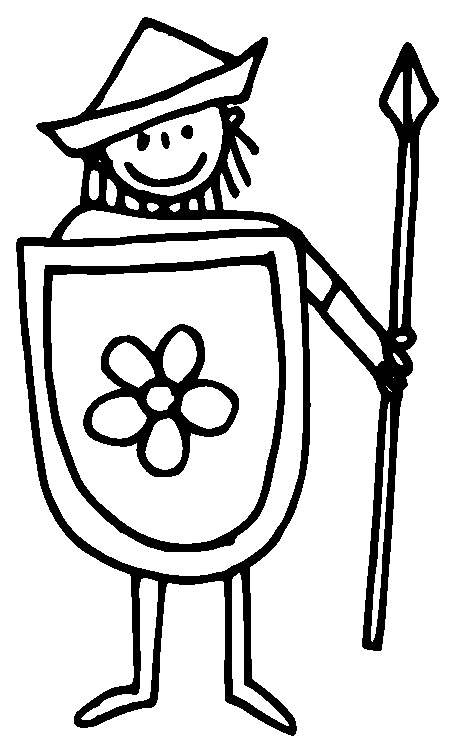
\includegraphics[width=7cm]{images/3.eps}
\vfil
\pagebreak
\section{Jsem zde na zemi poutníkem}
\begin{enumerate}
\item \Ch{C}{Jsem}\Ch{G7}{ }zde na zemi \Ch{C}{poutníkem} \\*
\Ch{C}{v prachu}\Ch{G7}{ } zmatených \Ch{C}{stop} \Ch{G7}{ } \\*
\Ch{C}{Bloudím} \Ch{G7}{ } přece však \Ch{C}{zpívám} všem \\*
kdo hledí na svůj \Ch{C7}{hrob} 
\item[Ref.:] \Ch{F}{Zpí}\Ch{G7}{vám} o tom \Ch{C}{že} nalé\Ch{a}{zám} \\*
cestu \Ch{d}{již} ze smr\Ch{G7}{ti} do ne\Ch{C}{be} \Ch{C7}{ } \\*
\Ch{F}{Bůh} \Ch{G7}{sám} který \Ch{C}{svět} \Ch{E7}{stvořil} \Ch{a}{nám} \\*
úděl \Ch{d}{nás }lidí \Ch{G7}{vzal} na se\Ch{C}{be} 
\item Na své pouti když hledám cíl \\*
skrytý před tváří mou \\*
v světě kde člověk ve tmách žil \\*
zřím hvězdu zářivou \\*
\end{enumerate}
 % 21
%\vfil
\begin{TEXT}{Každý den}
\SLOKA[] Každý \Ch{D}{den} Pán mi \Ch{G}{sí}lu dá\Ch{D}{vá} \NL
\Ch{D}{písní} mou je \Ch{G}{můj} \Ch{A}{Pán} \NL
On se \Ch{G}{stal} mým \Ch{F#}{spase}\Ch{h}{ním} \NL
když \Ch{A}{krá}čím \Ch{D}{s ním} nemu\Ch{G}{sím} se \Ch{D}{bát}  \NL
když \Ch{f#}{kráčím} \Ch{h}{s ním} nemu\Ch{G}{sím} \Ch{A}{se} \Ch{D}{bát}
\end{TEXT}
 % 22
\vfil
\pagebreak
\begin{TEXT}{Kdo mě z pout mých}
\REFREN  Kdo mě \Ch{E}{z pout} mých ven vy\Ch{E7}{vodí} \NL
kdo ta \Ch{A}{pouta} odstra\Ch{E}{ní} \Ch{H7}{ } \NL
jenom \Ch{E}{láska} vysvobo\Ch{E7}{dí} \NL
láska \Ch{A7}{bázeň} vyhá\Ch{E}{ní} \Ch{H7}{ } 
\SLOKA Být jak strom co plody nese \NL
nejen listí pro krásu \NL
být jak strom co neohne se \NL
nebojí se nečasu 
\SLOKA Být jak dům na skále pevné \NL
jako maják na moři \NL
se kterým ani příval nehne \NL
když se na něj oboří 
\REFRENHRAJ  
\SLOKA Pramen žití někde najít \NL
neznat co je únava \NL
třeba sám dál pravdu hájit \NL
i když právě prohrává 
\SLOKA Kdybych pronik' do atomu \NL
kdybych létal na Měsíc \NL
jako anděl mluvil k tomu \NL
lásku neměl nejsem nic 
\REFRENHRAJ 
\end{TEXT}
 % 23
\section{Kdo na kolenou klečí}
\begin{enumerate}
\item Kdo \Ch{e}{na} kolenou klečí \Ch{H7}{vídá} \Ch{e}{dál} \Ch{D}{ } \Ch{G}{ } \\*
\Ch{D}{Kdo} \Ch{e}{na} kolenou klečí vídá \Ch{a}{dál} \Ch{e}{ }
\item[Ref.:] Život \Ch{e}{svůj} \Ch{e7}{prý} kdo \Ch{e6+}{ztratí} \\*
jen \Ch{e}{ten} ho \Ch{a}{zachrá}\Ch{e}{ní} \\*
\Ch{C}{ } Dlou\Ch{e}{hý}, \Ch{a}{těž}\Ch{G}{ký} je \Ch{H7}{chápá}\Ch{e}{ní} \Ch{A}{ } \Ch{e}{ }
\item /: Kdo nedělá moc řečí poví víc :/
\item /: Kdo dává, zpět nežádá, má dost sám :/
\end{enumerate}
 % 24
\pagebreak
\section{Kdo stvořil}
\begin{enumerate}
\item \Ch{C}{Kdo} \Ch{G}{stvo}řil \Ch{C}{třpy}tící se hvězdy \\*
/: \Ch{G(C)}{třpytící} se hvězdy :/ \\*
\Ch{C}{kdo} \Ch{G}{stvo}řil \Ch{C}{třpy}tící se hvězdy \\*
\Ch{C}{náš} \Ch{G}{Otec} \Ch{C}{Bůh}
\item … létající ptáky…
\item … vlnící se moře… 
\item … celou naši zemi… 
\item … tebe jeho i mne… 
\item Bůh stvořil třpytící se hvězdy \\*
létající ptáky vlnící se moře \\*
Bůh stvořil celou naši zemi tebe i mne. 
\item[] (Mezi 5. a 6. sloku          možno vložit další, např.: \\*
velikánské slony, píchající ježky, půdní baktérie… )
\end{enumerate}
 % 25
\vfil
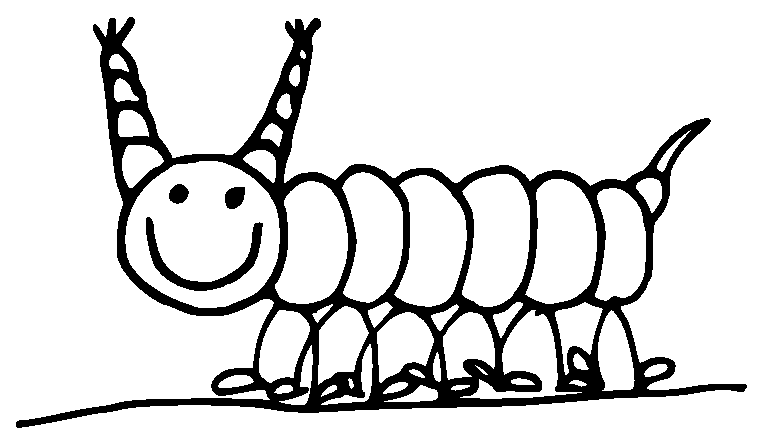
\includegraphics[width=12cm]{images/4.eps}
\vfil
\section{Koho včelky chválí}
\begin{enumerate}
\item \Ch{C}{Koho} včelky chválí pílí             nezměrnou \\*
kampak broučci malí zas \Ch{G}{míří} s lucernou \\*
\Ch{C}{kdo} je známý ještě jako tvůrce řek \\*
taky kapky deště co \Ch{G}{dává} žízni flek 
\item[Ref.:] /: Dobrý \Ch{C}{Bůh} \Ch{F}{náš} \Ch{C}{Pán}  Bůh \Ch{F}{náš} \Ch{C}{Pán} \\*
\Ch{d}{moudrý} \Ch{C}{štědrý} dárce \Ch{G}{Bůh} náš \Ch{C}{Pán} :/ 
\item Podívejme sovy mají zvláštní řád \\*
v noci dlouho loví a ráno chodí spát \\*
a co teprv brouci jaká těch je změť \\*
jen Bůh všemohoucí zná všechny nazpaměť 
\item Kdo se stará aby létal dětem drak \\*
učí malé žáby zakvákat kvaky kvak \\*
kdo dál žehná zemi i když je maličká \\*
kdo je mezi všemi na světě jednička 
\item On jak žádný druhý měsíc mění v srp \\*
zebrám dává pruhy a velbloudovi hrb \\*
jitrnice vepři vlnu ovečkám \\*
s ním je člověk ve při \\*
když na vše stačí sám \\*
\end{enumerate}
 % 26
\section{Kříž}
\begin{enumerate}
\item[Ref.:] /: \Ch{d(G)}{Láskou} svou nás Pane :/ \\*
\Ch{F}{láskou} \Ch{C}{svou} nás pozve\Ch{d}{dáš} \Ch{G}{ } \\*
/: \Ch{d(G)}{Kříže}m svým dál Pane :/ \\*
\Ch{F}{křížem} \Ch{C}{svým} zvedáš kříž \Ch{d}{náš} \Ch{(G)}{ } 
\item \Ch{d}{Ve} chvílích \Ch{A7}{neji}stot \Ch{F}{člo}věku \Ch{D7}{nab}ízíš \\*
\Ch{g(7)}{jedin}ý \Ch{C}{pev}ný bod \Ch{B}{na} zemi, tvůj \Ch{F}{kříž} \Ch{G}{ } 
\item Ovečkám ztraceným záchranu přinášíš \\*
v bloudění kéž je jim majákem tvůj kříž \\*
\end{enumerate}
 % 27
\vfil
\section{Kumbaja}
\begin{enumerate}
\item \Ch{D}{Př}ijď k nám Pane náš, \Ch{G}{ku}mba\Ch{D}{ja} \\*
Přijď k nám \Ch{f#}{Pane} náš, \Ch{e}{ku}mba\Ch{A}{ja}, \Ch{A7}{ } \\*
\Ch{D}{Př}ijď k nám Pane náš, \Ch{G}{ku}mba\Ch{D}{ja} \\*
/: \Ch{G}{ó} \Ch{D}{Pa}ne, \Ch{A}{kum}ba\Ch{D}{ja}:/ 
\item Vidíš nás svůj lid, kumbaja, \\*
přišli jsme tě ctít, kumbaja, \\*
vždyť ty jsi náš štít, kumbaja, \\*
/: ó Pane, kumbaja :/ 
\item V pokoře uč žít, kumbaja, \\*
společně dej jít, kumbaja, \\*
chlebem svým nás syť, kumbaja, \\*
/: ó Pane, kumbaja :/ 
\item Cestu ukazuj, kumbaja, \\*
věrně při nás stůj, kumbaja \\*
slyšet dej hlas svůj, kumbaja, \\*
/: ó Pane, kumbaja :/ 
\item Svobodu nám dej, kumbaja, \\*
zlo v nás přemáhej, kumbaja \\*
dveře otvírej, kumbaja, \\*
/: ó Pane, kumbaja :/ \\*
\end{enumerate}
 % 28
\vfil
\section{Laudato sii}
\begin{enumerate}
\item[Ref.:] /: \Ch{E(c#,A,H)}{Laudato sii o mi Signore} :/ 4x 
\item \Ch{E}{Dík} za všechno cos' stvořil Pane \\*
\Ch{c#}{dík} za teplo když slunce plane \\*
\Ch{A}{dík} za hvězdy za vánek svěží \\*
\Ch{H}{dík} za vodu za hudbu z věží 
\item Dík za vesmír planetu Zemi \\*
dík za chvíle kdy dobře je mi \\*
za přírodu když všechno vzkvétá \\*
moře hory za krásu světa 
\item Za to všechno díky vzdáváme \\*
spolu s bratry žalmy zpíváme \\*
ať každý z nás zblízka i zdáli \\*
celým srdcem tě Pane chválí
\item[] /: Celým srdcem tě Pane chválím :/ 4x
\end{enumerate}
 % 29
\section{Moudrost mi Pane dávej}
\begin{enumerate}
\item \Ch{G}{Mou}drost\Ch{D}{ mi} Pane \Ch{G}{dá}vej \Ch{D}{abych} po tvé \Ch{G}{ces}\Ch{C}{tě} \Ch{D}{chodil} \\*
\Ch{G}{mou}drost\Ch{D}{ mi} Pane \Ch{e}{dá}vej \Ch{a}{ať} ve tmě \Ch{D}{neblou}\Ch{G}{dím} \\*
\Ch{D}{mou}drost mi dávej \Ch{G}{sám} ji \Ch{(D)}{ne}m\Ch{G}{ám} \\*
\Ch{D}{mou}drost mi dávej \Ch{G}{ať} \Ch{C}{tě} \Ch{D}{hle}dám \\*
\Ch{G}{mou}drost\Ch{D}{ mi} Pane \Ch{e}{dá}vej \Ch{a}{ať} ve tmě \Ch{D}{neblou}\Ch{G}{dím} \\*
\end{enumerate}
 % 30

\section{Nám Pane dal jsi slovo své}  %laudate
\begin{enumerate}
\item[Ref.:] Nám \Ch{F}{Pan}e \Ch{a}{dal} jsi \Ch{A7}{slovo} \Ch{d}{své } \\*
\Ch{B}{Ducha} svého \Ch{C7}{dej} nám \Ch{F}{též} \Ch{C}{ } \\*
ať \Ch{F}{tebe} \Ch{a}{vždycky} \Ch{A7}{přijme}\Ch{d}{me}  \\*
\Ch{B}{Ducha} svého \Ch{C7}{dej} nám \Ch{F}{též}
\item Zůstaň \Ch{F}{Pane} s námi \Ch{a}{všechny} dny až \Ch{A7}{na vě}\Ch{d}{ky}\\*
\Ch{B}{Ducha} svého \Ch{C7}{dej} nám \Ch{F}{též} \Ch{C}{ } \\*
Ty jsi \Ch{F}{cesta} ty jsi \Ch{a}{život} pro nás \Ch{A7}{pro bra}\Ch{d}{try} \\*
\Ch{B}{Ducha} svého \Ch{C7}{dej} nám té\Ch{F}{ž} \Ch{B}{ } \Ch{F}{ }
\item Všechny moci světa když nás Pane týrají \\*
Ducha svého dej nám též \\*
ve víře nás přece Boží síla provází \\*
Ducha svého dej nám též 
\item Stále znovu zpívám Pane dej nám Ducha též \\*
Ducha svého dej nám též \\*
který srdce, mysl zarmoucenou pozdvihne \\*
Ducha svého dej nám též \\*
\end{enumerate}
 % 31
\vfil
\section{Někdo mě vede za ruku}
\begin{enumerate}
\item Ně\Ch{D}{kdo} \Ch{A}{mě} \Ch{D}{ve}\Ch{A}{de} \Ch{D}{za} ru\Ch{D7}{ku }když \Ch{G}{bojím} se jít \Ch{D}{tmou} \Ch{A7}{ }\\*
to \Ch{D}{je }ten \Ch{A}{který} \Ch{D}{o }\Ch{F#}{mně} \Ch{h}{ví} \Ch{A}{kte}\Ch{D}{rý} je \Ch{D7}{na} mě \Ch{e}{las}ka\Ch{A}{vý }\\*
je \Ch{D}{stá}\Ch{h}{le} \Ch{e}{na}\Ch{A7}{de }\Ch{D}{mnou} 
\item Někdo mi dává denní chléb že nemusím mít hlad \\*
to je ten který o mně ví který je na mě laskavý \\*
a chce mi pomáhat 
\item Někdo mi dává sílu též když už jsem unaven \\*
to je ten který o mně ví který je na mě laskavý \\*
ať je noc nebo den 
\item Někdo mě vede za ruku proto se nechci bát \\*
to je ten který o mně ví můj dobrý Pán Bůh laskavý \\*
který mě má tak rád \\*
\end{enumerate}
 % 32
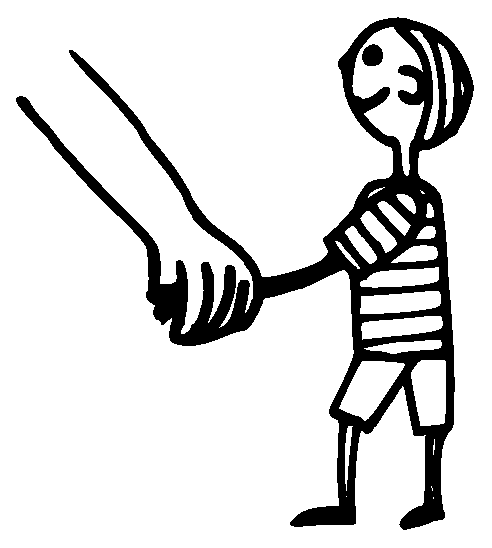
\includegraphics[width=8cm]{images/5.eps}
\pagebreak
\begin{TEXT}{Není lepší na tom světě}
\SLOKA \Ch{D}{Není} \Ch{G}{lep}ší \Ch{D}{na tom} \Ch{e}{světě} \Ch{D}{než}li \Ch{a}{Boha} ctí\Ch{D}{ti} \NL
jeho vzý\Ch{D7}{vat} \Ch{G}{jemu} slou\Ch{e}{žit} \Ch{G}{jeho}\Ch{e}{ ve}\Ch{a}{le}\Ch{D}{bit}\Ch{G}{i } 
\SLOKA Není lepší na tom světě nežli druhým dávat \NL
však bohatství s jeho strastí ani nepoznávat 
\SLOKA Není lepší na tom světě než v pokoji bývat \NL
místo zlostí mrzutostí Pánu Bohu zpívat 
\SLOKA Není lepší na tom světě než svědomí čisté \NL
to nám dávej uchovávej milý Pane Kriste \NL
\end{TEXT}
 % 33
\begin{TEXT}{Nevím Pane}
\SLOKA \Ch{E}{Ne}vím Pane\Ch{A}{ co} ti \Ch{E}{dát} nevím \Ch{c#}{jak} ctít \Ch{f#}{Tebe} \Ch{H7}{ }\NL
\Ch{f#}{že jsem} mohl \Ch{G#}{dobře} \Ch{c#}{spát} \Ch{f#}{a že} \Ch{H}{vi}dím \Ch{E}{ne}be 
\SLOKA Nevím Pane jak dát znát že chci tobě věřit \NL
že chci bližní milovat víru láskou měřit 
\SLOKA Věřím Pane že ty víš co je v lidském nitru \NL
dřív vše za mne vyslovíš než dáš vzplanout jitru 
\SLOKA Proto přetvoř srdce mé ať to není kámen \NL
/: Dej mi radost a chuť žít za to prosím. Amen :/ \NL
\end{TEXT}
 % 34
\begin{TEXT}{Odpusť}
\SLOKA \Ch{C}{Od}pusť\Ch{e}{ že} dnes tak \Ch{d}{ja}ko \Ch{G}{vče}ra \NL
\Ch{C}{ jsem} tobě \Ch{e}{věr}nost \Ch{d}{sli}bo\Ch{G}{val} \NL
\Ch{C}{odpusť}\Ch{E7}{ že zrána} \Ch{A}{do ve}\Ch{f}{če}ra \NL
\Ch{C}{ jsem} tebe \Ch{d}{skut}kem \Ch{G7}{zrazo}\Ch{C}{val} \Ch{C7}{ } \NL 
\Ch{F}{odpusť}\Ch{f}{ že zrána} \Ch{C}{do ve}če\Ch{A}{ra} \NL
\Ch{d}{ jsem} tebe \Ch{G7}{sku}tkem zrazo\Ch{C}{val}
\SLOKA Odpusť že jsem nevyslech' bratra \NL
který se mne na radu ptal \NL
/: odpusť že jsem se díval spatra \NL
na toho který klopýtal :/ 
\SLOKA Odpusť že nad svou hněvivostí \NL
nechal jsem slunce zapadnout \NL
/: odpusť že jsem dnes bez milosti \NL
slepého nechal upadnout :/ 
\SLOKA Odpusť mi Pane zase znova \NL
odpusť mi každý lásky dluh \NL
/: odpusť všechna zbytečná slova \NL
odpusť jenž slitovný jsi Bůh :/ \NL
\end{TEXT}
 % 35
\begin{TEXT}{Otevřete brány}
\SLOKA \Ch{E}{Otevřete} brány hradeb \Ch{E7}{kamenných} \NL
\Ch{A}{otevřete} brány hradeb \Ch{Edim}{srdcí svých} \NL
\Ch{E}{otevřete} \Ch{c#}{aby mohl} \Ch{f#}{dál} \Ch{H7}{ } \NL
\Ch{E}{nechte} všeho nechte obav \Ch{E7}{starostí} \NL
\Ch{A}{připravujte} cestu jeho \Ch{Edim}{království} \NL
\Ch{E}{připravujte} \Ch{c#}{cestu} aby \Ch{F#}{vejít} mohl \Ch{H}{slávy} kr\Ch{E}{ál }
\REFREN  To kvůli krá\Ch{E7}{li,} \Ch{A}{krá}\Ch{Edim}{li }\Ch{E}{při}prav \Ch{c#}{každý} cestu \NL
\Ch{F#}{cestu} \Ch{H7}{svou} \NL
to kvůli \Ch{E}{krá}\Ch{E7}{li,} \Ch{A}{krá}\Ch{Edim}{li }\Ch{E}{naprav} \Ch{c#}{každý} cestu \NL
\Ch{F#}{cestu} křivou \Ch{H7}{cestu} \Ch{E}{zlou }
\SLOKA Pozdvihněte svoje srdce znavená \NL
posilněte klesající kolena \NL
otevřete aby mohl dál \NL
není doba k spánku je čas nabrat sil \NL
pominula noc a den se přiblížil \NL
připravujte cestu aby vejít mohl slávy král \NL
\end{TEXT}
 % 36
\hspace*{2cm}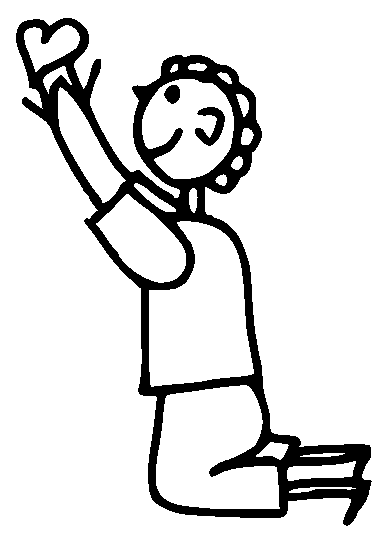
\includegraphics[width=3cm]{images/6.eps}
\begin{TEXT}{Pane slyš náš hlas}
\SLOKA[] \Ch{D}{Pane} \Ch{C}{slyš náš} \Ch{H7}{hlas} \NL
\Ch{e}{chcem} Tě \Ch{E7}{chválit} \Ch{A}{zas} \NL
/: \Ch{D}{za to} \Ch{C}{že máš} \Ch{H7}{v pé}či \Ch{e}{ce}lý \Ch{A7}{svět} i \Ch{D}{nás} :/ \NL
\end{TEXT}
 % 37
\vfil
\begin{TEXT}{Pán Bůh nás má všechny rád}
\SLOKA \Ch{D}{Pán} Bůh nás má \Ch{A7}{vše}chny rád \NL
a \Ch{G}{odpou}ští nám každý \Ch{A7}{den} \NL
\Ch{D}{pro}to také \Ch{A}{chce}me se mít \Ch{G}{rá}di \Ch{A7}{navzá}\Ch{D}{jem}
\SLOKA Volá k sobě všechny děti: Děti pojďte sem\,! \NL
Zvu vás všechny do království \NL
kdo chce pojďte jdem. \NL
\end{TEXT}
 % 38
\pagebreak
\begin{TEXT}{Plné ruce plná ústa díků}
\SLOKA \Ch{C}{Plné} ruce \Ch{G}{plná} ústa \Ch{C}{díků} \NL
každý den vždy \Ch{G}{nový} důvod \Ch{C}{mít} \Ch{C7}{}\NL
\Ch{F}{chvá}lu vzdávat \Ch{G}{bez} frází a \Ch{a}{zvyků} /: \Ch{F}{nauč} nás\Ch{C(G)}{ žít :/}\NL
\Ch{C}{Stě}ží chápem, \Ch{G}{co} se denně \Ch{C}{stá}vá \NL
jenom vírou \Ch{G}{je} to možné vzít \Ch{C7}{}\NL
\Ch{F}{a kdo} ví to \Ch{G}{zpívat} nepře\Ch{a}{stá}vá 
\REFREN  \Ch{F}{ Halelu}\Ch{C}{ja} \Ch{F}{ my ty i} \Ch{C}{já} \Ch{F}{ halelu}\Ch{C}{ja} ať zní \Ch{G}{chvá}la jása\Ch{a}{vá } \NL
/: \Ch{F}{hale}lu\Ch{C}{ja} :/     \Ch{F}{hale}lu\Ch{C}{ja} ať zní \Ch{G}{chvá}la jása\Ch{C}{vá}  
\SLOKA Plné oči plná ústa chvály \NL
tolik pěkných věcí kolem nás \NL
nezahálí kdo v životě chválí /: dál půjde snáz :/ \NL
Každému ať zazní dobrá zpráva \NL
aby spásu nikdo nepropás' \NL
a kdo ví to zpívat nepřestává 
\SLOKA La la la… \NL
Všem lidem své dary Pán Bůh dává \NL
není kdo by s prázdnou musel jít \NL
a kdo ví to zpívat nepřestává \NL
\end{TEXT}
 % 39
\begin{TEXT}{Posila na cestu}
\SLOKA \Ch{C}{K svo}bodě je \Ch{G}{dlou}hé puto\Ch{a}{vá}n\Ch{C7}{í    }  \NL
\Ch{F}{těž}ké bývá \Ch{f}{zved}nout se a \Ch{d7}{jít} \Ch{G}{ } \NL
\Ch{C}{Tolik} různých \Ch{E7}{pout} tolik \Ch{a}{zá}vor \Ch{C7}{v ce}stě brání \NL
\Ch{F}{jen} sám Bůh je \Ch{G}{umí} rozlo\Ch{C}{mit} \Ch{(G)}{ }  
\SLOKA V noci naplněné odhodláním \NL
v noci která je tou poslední \NL
Beránek a chléb, v ruce hůl a žádné spaní \NL
za zdmi domů krví značených 
\SLOKA Na úsvitu voda staré splaví \NL
stíny zákeřného otroctví \NL
Cesta míří dál celý průvod jde před námi \NL
směr udává nám sloup ohnivý 
\SLOKA Každý kdo se dlouhou cestou znaví \NL
zadarmo se vína napít smí \NL
dostává i chléb, novou sílu z Božích dlaní \NL
víru že smrt končí vzkříšením \NL
\end{TEXT}
 % 40
\vfil
\begin{TEXT}{Povím vám teď}
\SLOKA \Ch{D}{Povím} vám teď jakou radost mám \NL
smutnou pré\Ch{A}{rií}  když \Ch{G}{jedu} \Ch{D}{sám} \Ch{G}{ } \Ch{D}{ }
\SLOKA Cesta skalnatá kudy se mám brát \NL
kde najdu klid koho mám mít rád 
\SLOKA Temná je noc jasný je cíl \NL
v Boží ochraně bude vždy můj díl 
\end{TEXT}
 % 41
\section{Přímluvný zpěv}
\begin{enumerate}
\item \Ch{G}{Za ty,} \Ch{h}{kdo} hladem \Ch{C}{trpí} a \Ch{D}{bídou,}\\*
\Ch{e}{prosíme}: \Ch{D7}{Zjev} svoji \Ch{G}{slávu}\,! \\*
Za ty, \Ch{h}{kteří} \Ch{C}{druhými}  \Ch{e}{jsou} odmí\Ch{C}{tán}\Ch{D}{i} \\*                                                %\Ch{D}{ } \\*
\Ch{G}{prosíme:} \Ch{D7}{Zjev} svoji \Ch{G}{slávu\,!} 
\item Za ty, kdo bolest mají a pláčí,\\*
prosíme: Zjev svoji slávu\,!\\*
Také za ty, kteří jsou svázáni pouty,\\*
prosíme: Zjev svoji slávu\,!
\item Za ty, kdo Slovo svaté tvé káží,\\*
prosíme: Zjev svoji slávu\,!\\*
Za ty, kteří ve jménu tvém bližním slouží,\\*
prosíme: Zjev svoji slávu\,!
\item Za ty, kdo světem bez lásky bloudí,\\*
prosíme: Zjev svoji slávu\,!\\*
Za ty, kteří jsou stále nám protivníky,\\*
prosíme: Zjev svoji slávu\,!
\item A tak pro Krista, svatého Pána,\\*
prosíme: Zjev svoji slávu\,!\\*
Učiň, celý svět náš ať v míru tě chválí\,!\\*
Prosíme: Zjev svoji slávu\,! Amen\\*
\end{enumerate}
 % 42
\section{Ranní prosba}
\begin{enumerate}
\item \Ch{D}{Pro}síme tě, \Ch{A}{Pa}ne, buď \Ch{C}{s námi} celý \Ch{G}{den,} \\*
ať \Ch{D}{ve} všem, co se \Ch{A}{stane}, jsi \Ch{C}{námi} osla\Ch{G}{ven.} 
\item[Ref.:] Pane \Ch{D}{náš,} prosíme, \Ch{A}{dej,} \\*
ať \Ch{G}{smutek} není \Ch{f#}{králem} a \Ch{e}{bolest} princez\Ch{D}{nou},\\*
\Ch{h}{slun}ce ať má \Ch{A}{správ}ný \Ch{D}{jas}, \\*
\Ch{G}{v to}bě pravou \Ch{f#}{radost} ať \Ch{e}{smut}ní nale\Ch{D}{znou,} \\*
\Ch{A}{pro}síme tě, \Ch{A7}{vyslyš} nás.
\item Ať přestáném se mračit a dokážem se smát,\\*
ať umí znovu začít ten, koho zastih' pád.
\item Ať postavíme chrámy z tvé lásky v srdcích svých,\\*
buď celý dnešek s námi, ať přemůžeme hřích.
\item Ať nejdem spát s otázkou, co ty nám zítra dáš,\\*
ať všechno přijmem s láskou, jak ty nás přijímáš. \\*
\end{enumerate}
 % 43
\begin{TEXT}{Rok za rokem}
\REFREN  \Ch{C}{Rok za} \Ch{F}{rokem} \Ch{D}{roky,} \Ch{G}{léta} \Ch{C}{jdou}, k roku \Ch{F}{rok,} \NL
v ruku \Ch{d}{laskavou}, ó \Ch{C}{Pane} \Ch{E7}{v ruku} \Ch{a}{tvo}\Ch{C7}{u}   \NL
\Ch{F}{Vkládám} dny a \Ch{D}{ro}ky \Ch{G}{tak, jak} \Ch{C}{jdou.}
\SLOKA \Ch{C}{Znám} \Ch{F}{ča}sy, \Ch{G}{kdy} tě \Ch{C}{smích} opus\Ch{F}{tí,} \NL
vím o těch \Ch{d}{dobách} zlých, \NL
vím \Ch{C}{o ú}\Ch{E7}{horu,} \Ch{a}{bod}lá\Ch{a7}{čí,} \NL
\Ch{D}{ } o dechu, který \Ch{G}{nestačí,} ó
\SLOKA Znám léta zářivá,\NL
hojný stůl a kalich oplývá\NL
a píseň chválí růst i žeň,\NL
natisíckrát jsi obdařen. 
\SLOKA Svou ruku do dlaní\NL
silnějších, než je mé doufání,\NL
já vložím s dechem posledním,\NL
za řekou času zemi zřím. \NL
\end{TEXT}
 % 44
\begin{TEXT}{Řekl tobě}
\SLOKA /: Řekl \Ch{D}{to}bě tvůj \Ch{G}{Bůh} \NL
co je \Ch{A}{do}bré a co \Ch{G}{On} od tebe \Ch{D}{žá}dá :/ 
\SLOKA /: Abys byl přímý a milosrdný \NL
pokorně chodil s Bohem svým :/ \NL
\end{TEXT}
 % 45
\section{Slunce v rose koupalo se}
\begin{enumerate}
\item \Ch{D}{Slunce} v rose \Ch{G}{koupa}\Ch{D}{lo} se \Ch{e}{z lesů} \Ch{A}{při}šla \Ch{D}{noc}\\*
\Ch{D}{Pán Bůh} \Ch{D7}{s námi} \Ch{G}{ať nás} \Ch{D}{chrání} \Ch{e}{od} zla \Ch{A7}{jeho} \Ch{D}{moc} 
\item A tam v dáli hvězdy vzplály všichni půjdem spát \\*
tiše tiše pro Ježíše má nás Pán Bůh rád 
\item (Pac a zbrusu novou pusu a už půjdem spát \\*
nezbedníky díky díky dál má někdo rád) \\*
\end{enumerate}
 % 46
\vfil
\section{Sluníčko lechtá žabky v kaluži}
\begin{enumerate}
\item \Ch{C}{Slu}níčko \Ch{F}{lechtá} žabky \Ch{C}{v kaluži} \\*
\Ch{C}{vrabec} ten \Ch{F}{pro}mokl až \Ch{C}{na} kůži \\*
\Ch{C}{ží}\Ch{a}{ža}\Ch{G}{la} \Ch{C}{zí}\Ch{G}{va}\Ch{C}{la} prý \Ch{a}{ten} \Ch{G}{déšť} zaspa\Ch{C}{la} 
\item Díky ó Pane Bože šťastný jsem \\*
díky za život nebe krásnou zem \\*
nechci se kabonit vím že je krásné žít \\*
\end{enumerate}
 % 47
\pagebreak
\begin{TEXT}{Spoj nás v jedno Pane}
\SLOKA* \Ch{D}{Spoj} nás v jedno Pane \Ch{h}{spoj} nás v jedno poutem \NL
\Ch{e}{jež} ne\Ch{A}{může} být \Ch{D}{zlámáno} \NL
\Ch{D}{spoj} nás v jedno Pane \Ch{h}{spoj} nás v jedno poutem \NL
\Ch{e}{spoj} nás v jed\Ch{A}{no} láskou \Ch{D}{svou} 
\REFREN  \Ch{D}{Je} jen \Ch{A}{jeden} \Ch{D}{Bů}\Ch{h}{h} \Ch{D}{je} jen \Ch{A7}{jedno} \Ch{D}{tě}\Ch{A7}{lo } \NL
\Ch{D}{je} jen \Ch{A}{jeden} \Ch{D}{Pá}\Ch{h}{n} \Ch{D}{pro}to \Ch{A7}{zpívá}\Ch{D}{me:} \Ch{A}{ }   \NL
Spoj nás v jedno Pane… \NL
\end{TEXT}
 % 48
\section{Stádo}
\begin{enumerate}
\item[Ref.:] \Ch{G7}{Stádo} \Ch{F}{stádo} ovcí máš \\*
Pastýři jakej div \Ch{C}{že} se v něm vyznáš \\*
Pastýři za málo \Ch{F}{za} málo's mu stál \\*
jakej zázrak že\Ch{C}{ }mě stále čekáš \\*
když víš\Ch{G}{ }co jsem za\Ch{C}{č } 
\item \Ch{F}{Vlast}ním autem vlastní cestou \\*
\Ch{C}{stí}háme svůj vlastní cíl \\*
\Ch{F}{v tou}ze stát na vlastní noze \\*
\Ch{C}{ne}šetříme vlastních sil \\*
\Ch{F}{Ně}co ex pro sebe mít \\*
\Ch{C}{jen} se tlačit jen se bít \\*
\Ch{D7}{vlast}ní to lidskej \Ch{G7}{nápad} byl 
\item Vsadil jsem na vlastní rozum \\*
nic nenechám náhodám \\*
žiju si na velký noze \\*
ouzkejm cestám uhejbám \\*
ve svý vlastní víře \\*
pást se bez Pastýře \\*
hloupý se ovci podobám
\end{enumerate}
 % 49
\section{Stále stále}
\begin{enumerate}
\item[Ref.:]    \Ch{D6}{Stále} \Ch{D}{stále} \Ch{G}{zůstávej} \Ch{A}{s námi} Pane \\*
\Ch{D6}{stále} \Ch{D}{stále} a \Ch{e}{neo}\Ch{E7}{pouštěj} \Ch{A7}{nás} \\*
\Ch{D}{o krok} dá\Ch{D7}{le} \Ch{G}{na} ces\Ch{H7}{tě} nás \Ch{e}{veď} \\*
\Ch{E7}{stále} \Ch{D}{teď} a \Ch{A}{v každý} \Ch{D}{čas} \Ch{D7}{} 
\item \Ch{G}{Pů}jdu kam mě pošle Pán nebojím se nejsem sám \\*
\Ch{a}{pro} něj dýchat \Ch{G}{chci} a \Ch{a}{žít}\Ch{D}{ } \\*
\Ch{a}{pokoj} v srdci \Ch{D}{nést} \Ch{G}{lidi} v bratry \Ch{e}{proměnit} \\*
\Ch{a}{hlásat} \Ch{D}{blahou} \Ch{G}{zvěst} \Ch{A7}{ }
\item V bouři ani temnotách nebojím se nemám strach \\*
věřím v slunce nad mraky našich těžkých chvil \\*
Kristus činí zázraky ukazuje cíl 
\end{enumerate}
 % 50
\vfil
\hspace*{3cm}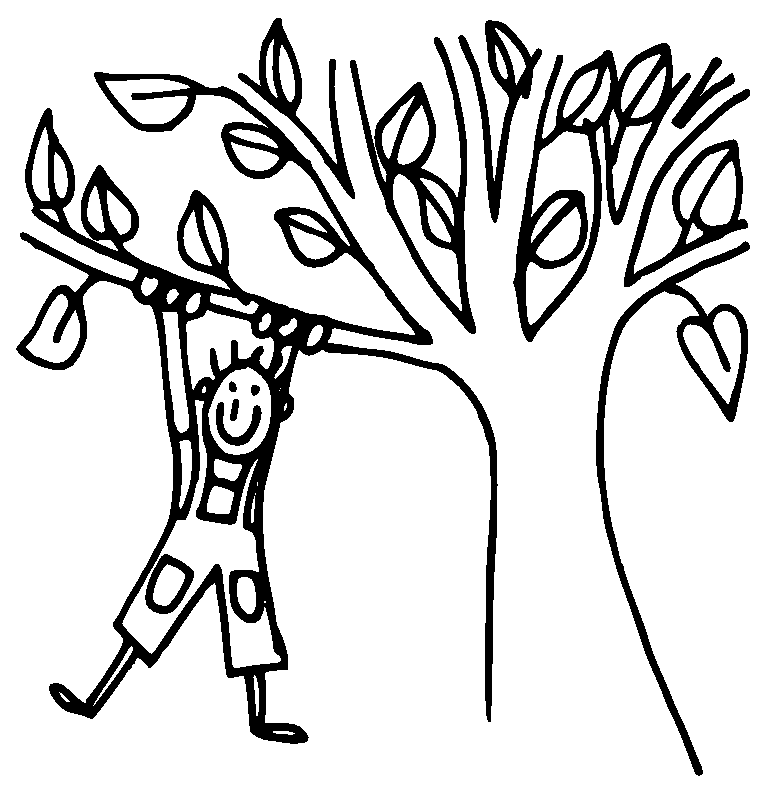
\includegraphics[width=10cm]{images/7.eps}
\vfil
\section{Svý kroky rozezpívej}
\begin{enumerate}
\item[Ref.:] \Ch{d}{Svý} kroky \Ch{C}{rozezpí}v\Ch{F}{ej,} \Ch{G}{rozezpí}v\Ch{B}{ej,} \Ch{C}{rozezpí}v\Ch{a}{ej}  \\*
\Ch{d}{chválama} \Ch{C}{rozezpí}v\Ch{F}{ej,} \Ch{G}{rozezpí}v\Ch{B}{ej,} \Ch{C}{rozezpí}v\Ch{D}{ej} 
\item \Ch{d}{Vzdejme} Pánu díky \Ch{G}{za }vše co nám dává \\*
\Ch{B}{za vše} co nám bere \Ch{A}{patří} Pánu sláva \\*
vzdejme Pánu díky že se stará aby \\*
nepropadli smrti jeho lidé slabí 
\item Vzdejme Pánu díky novou cestu klestí \\*
v době která zná jen pomíjivé štěstí \\*
vzdejme Pánu díky křížem přišel říci \\*
já jsem cesta pravda osvobozující 
\item Vzdejme Pánu díky zdroji pravé spásy \\*
doutnající oheň láska neuhasí \\*
vzdejme Pánu díky jako děti Boží \\*
že v člověku láska lásku stále množí 
\item Vzdejme Pánu díky burcuje svým slovem \\*
starý svět už umřel my žijeme v novém \\*
vzdejme Pánu díky mění dávné řády \\*
Bůh už není v dálce Kristus žije tady 
\end{enumerate}
 % 51
\vfil
\hspace*{1cm}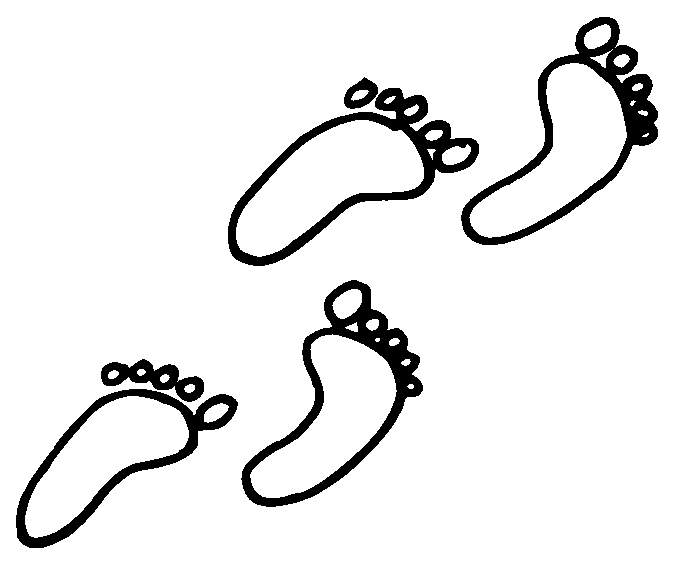
\includegraphics[width=7cm]{images/8.eps}
\vfil
\begin{TEXT}{Tobě Pane dík}
\REFREN  \Ch{G}{Tobě} \Ch{H7}{Pane} \Ch{e}{dík} že \Ch{C}{dal} jsi \Ch{D}{perlu} \Ch{G}{krásnou} \NL
Tobě \Ch{H7}{Pane} \Ch{e}{dík} že \Ch{C}{květy} \Ch{D}{mohou} \Ch{G}{kvést} \NL
Tobě Pane dík už vidím hvězdu jasnou \NL
Tobě Pane dík chceš s námi tíhu nést 
\SLOKA \Ch{a}{ Do} šera \Ch{e}{do} tmy\Ch{C}{ hvěz}da nám \Ch{G}{svítí} \NL
\Ch{a}{ do} temna \Ch{e}{noci} \Ch{C}{jasný} \Ch{D}{cíl} \NL
\Ch{a}{ V} tom světle \Ch{a}{člověk} \Ch{C}{naději} cítí \NL
\Ch{E}{ ze }světla čerpáš \Ch{a}{nejvíc} sil \Ch{a7}{ }
\SLOKA Pozdvihni oči pro tebe taky \NL
ta hvězda svítí nejsi sám \NL
I když ji někdy zakryjí mraky \NL
ozve se znovu Pokoj vám \NL
\end{TEXT}
 % 52
\begin{TEXT}{Tolik planých slov}
\SLOKA[] Tolik \Ch{G}{planých} slov jako \Ch{C}{prach} a \Ch{G}{dým} \NL
mi lítá kolem \Ch{D}{uší} \NL
ale \Ch{G}{dneska} jen Pane \Ch{C}{slovům} \Ch{G}{tvým} \NL
/: na\Ch{e}{slou}chám \Ch{D}{celou} \Ch{G}{duší} :/ \NL
Ať po\Ch{G}{znám} Bože \Ch{a}{můj}               \Ch{D}{jak} tě mít rád \NL
ať se \Ch{G}{líp} nau\Ch{a}{čím} \Ch{D}{tvé} písně \Ch{C}{hr}\Ch{a}{át} \Ch{D}{ } \NL
V srdci \Ch{G}{ro}zezvuč mých šest \Ch{C}{prá}zdných \Ch{G}{strun} \NL
/: ať \Ch{a}{sly}ší i \Ch{D}{ti} co jsou \Ch{G}{hlu}ší :/ \NL
Nas\Ch{e}{lou}chám \Ch{D}{celou} \Ch{C}{duší} \Ch{G}{ } 
\end{TEXT}
 % 53
\vfil
\section{Tvá svoboda}
\begin{enumerate}
\item /: \Ch{D}{Tvá} svo\Ch{G}{boda} :/ \Ch{D}{tvá} svo\Ch{e}{boda} nade \Ch{a}{mnou} \Ch{D7}{  } 
\item[Ref.:] Než a\Ch{G}{bych} byl otro\Ch{G7}{kem} \\*
chci být \Ch{C}{pohřben} v hrobě \Ch{G}{svém} \\*
\Ch{D}{půj}du \Ch{G}{k Pá}\Ch{e}{nu} kde \Ch{A7}{budu} \Ch{D7}{svobo}\Ch{G}{den} \Ch{C}{  } \Ch{G}{ } 
\item Žádný nářek… 
\item Zazpívejte… 
\item Zvony zvoňte… 
\item Slituješ se… 
\item Haleluja…
\end{enumerate}
 % 54
\vfil
\begin{TEXT}{Už k nám přišel brácha den}
\SLOKA \Ch{C}{Už} \Ch{G}{k nám} \Ch{C}{při}šel brácha den do pa\Ch{G}{prsků} oblečen \NL
volá \Ch{a}{Otvírejte} \Ch{F}{dobré} zprávy \Ch{C}{mám}\Ch{G}{! } \NL
Pěkně \Ch{C}{vyspal} se dnes les rosa \Ch{G}{sedá} na pařez \NL
dnešní \Ch{a}{představení} \Ch{F}{právě} začí\Ch{C}{ná} /: začí\Ch{G}{ná}\Ch{(C)}{ } :/ 
\REFREN  /: To všechno \Ch{a}{On} On On On ti \Ch{e}{dá}vá :/ \NL
\Ch{F}{abys} poznal \Ch{C}{jak} moc tě má \Ch{G}{rád} 
\SLOKA V hlavních rolích čistej vzduch \NL
ráj všech motýlů a much \NL
z pěvců postavili ptáci celej chór \NL
dále hrají louka les v lese pohádkovej vřes \NL
hráz a rybník starý necky malej vor /: malej vor :/ 
\SLOKA Kdo má oči na šťopkách vůbec nemusí mít strach \NL
že dnes večer půjde otrávenej spát \NL
všude známý režisér vybral nejkrásnější z her \NL
aby radost měl dnes každej kamarád /: kamarád :/ \NL
\end{TEXT}
 % 55
\pagebreak
\begin{TEXT}{Už mi oči tíží sen}
\SLOKA \Ch{D}{Už mi} \Ch{h}{oči} \Ch{e}{tí}\Ch{A}{ží} \Ch{D}{sen} \Ch{e}{a já} \Ch{D}{spát} jdu\Ch{f#}{ u}\Ch{E9}{nav}\Ch{A}{en } \NL
\Ch{D}{buď} \Ch{G}{mou} \Ch{D}{věr}\Ch{A}{nou} \Ch{D}{strá}\Ch{F#(7)}{ží } \Ch{h}{sám} \NL
Otče pro\Ch{A}{ti} \Ch{h}{noč}\Ch{A}{ním} \Ch{G}{tmám}
\Ch{D}{Ot}\Ch{h}{če} \Ch{e}{proti} \Ch{A7}{nočním} \Ch{D}{tmám}
\SLOKA Na zlé co jsem udělal nevzpomínej Pane dál \NL
pro Ježíše jeho kříž \NL
/:všechno v dobré obrátíš:/ 
\SLOKA A ty které mám tak rád rač mi Pane zachovat \NL
nad svým světem lítost měj \NL
/:všechněm lidem pomáhej:/ 
\SLOKA Srdcím nešťastným dej klid smutné ty rač potěšit \NL
Pane Bože tvoje moc \NL
/:dej nám všechněm dobrou noc:/ \NL
\end{TEXT}
 % 56
\vfil
\hspace*{1cm}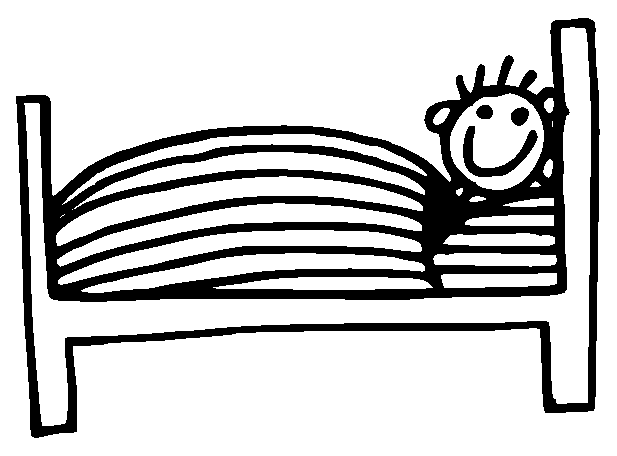
\includegraphics[width=10cm]{images/9.eps}
\vfil
\section{Už svítá jasný bílý den}
\begin{enumerate}
\item \Ch{A6}{Už} \Ch{h}{svítá} \Ch{A}{jasný} \Ch{D}{bí}\Ch{A}{lý} \Ch{D}{den} \\*
já \Ch{A}{k Bohu} \Ch{D}{v duchu} \Ch{G}{pokor}\Ch{A}{ném} \\*
se \Ch{D}{mo}d\Ch{F#}{lím} \Ch{h}{Tvá} se \Ch{G}{vůle} \Ch{A}{staň} \\*
buď \Ch{D}{Ty} má \Ch{A}{stráž} buď \Ch{h}{Ty} \Ch{e}{můj} \Ch{F#}{Pán} \\*
buď \Ch{e}{Ty} má stráž \Ch{G}{buď} \Ch{A7}{Ty můj} \Ch{D}{Pán}
\item Ať na     rtech nemám slovo zlé \\*
a srdce záští prolezlé \\*
ať nezotročí pohled můj \\*
/:když marnost láká při mně stůj:/ 
\item Ať přímost mého jednání \\*
přec tvrdosti se ubrání \\*
co tělo chce to zlom a ztiš \\*
/:hlad žízeň nebuď na obtíž:/ 
\item Až potom slunce zapadne \\*
a tma se vkrade v soumrak dne \\*
všech břemen svých a strachu prost \\*
/:zazpívám chválu za milost:/ 
\item Buď chvála Otci našemu \\*
i Synu jeho milému \\*
i Duchu v němž je útěcha \\*
/:budoucí dnešní odvěká:/
\end{enumerate}
 % 57
\vspace*{-0.5cm}\hspace*{7cm}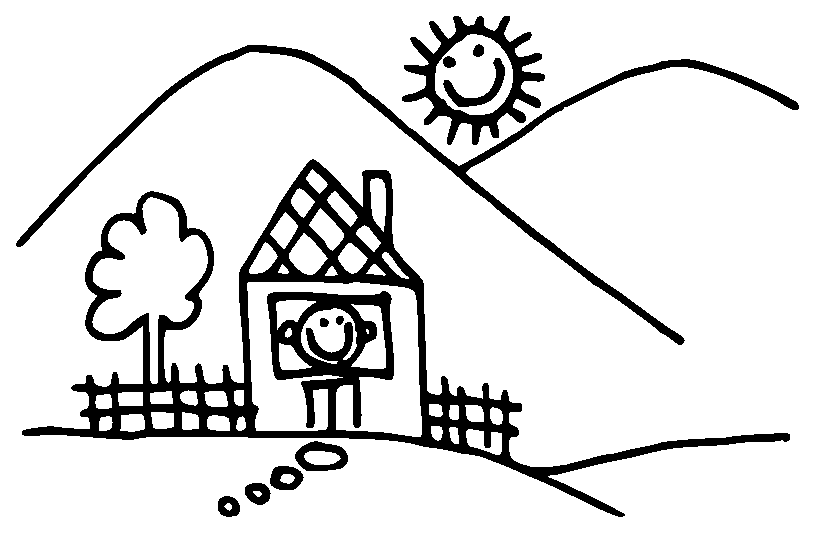
\includegraphics[width=7cm]{images/10.eps}\vspace*{-1cm}
\vfil
\begin{TEXT}{Veď mne dál}
\SLOKA[A.] \Ch{E}{Veď} mne dál Pane do svého království \NL
\Ch{H7}{veď} mne dál Pane i s mojí hloupostí \NL
\Ch{E}{veď} mne dál Pane navzdory nástrahám \NL
\Ch{H7}{ó veď} mne \Ch{E}{dál} 
\SLOKA[B.]Já málo síly k cestě mám \NL
sám spoustu škody nadělám \NL
smím víru mít že dojdu tam \NL
kam mě vede můj Pán 
\SLOKA[C.] /: Veď mne dál :/ 3x \NL
ó veď mne dál \NL
\end{TEXT}
 % 58
\pagebreak
\section{Ví}
\begin{enumerate}
\item \Ch{G}{Ví} Bůh kolik \Ch{h}{vlasů} spadne \Ch{e}{denně} lidem z hlav \\*\hspace*{1cm}-- \Ch{a}{ví} \Ch{G}{ví} \Ch{D}{ví} \\*
\Ch{a}{proč} jen někde \Ch{e}{chodí} děti \Ch{G}{domů} bez \Ch{D}{obav} \\*\hspace*{1cm}-- \Ch{G}{ví} \Ch{D}{ví} \Ch{C}{ví} \Ch{D}{ } \\*
\Ch{G}{ví} Bůh kolik \Ch{h}{mezi} ptáky \Ch{e}{pole}tuje strak -- \Ch{a}{ví} \Ch{G}{ví} \Ch{D}{ví} \\*
\Ch{a}{ko}lik černých \Ch{e}{pa}sažérů \Ch{C}{ve}ze který \Ch{D}{vlak} -- \Ch{G}{ví} \Ch{D}{ví} \Ch{G}{ví} 
\item[Ref.:]    Bůh dobře /: \Ch{a}{zná} \Ch{(D)}{mo}dřiny :/ \\*
\Ch{h}{špunta} který právě na zem \Ch{e}{spad} \\*
Bůh dobře /: \Ch{a}{ví} \Ch{(D)}{jak}          mu je :/ \\*
\Ch{C}{po}máhá \Ch{D}{mu} \Ch{G}{vstát} \Ch{(D)}{} 
\item Ví Bůh kolik zeměkouli stvořil kdysi řek -- ví… \\*
ví jak trápí šedý zákal oči studánek -- ví… \\*
ví jak málo stačí aby onemocněl smrk -- ví… \\*
ví Bůh proč se rybky z říčky daly na úprk -- ví… 
\item Ví Bůh kolik smutku znají chladné stěny cel -- ví… \\*
ví kdy vrátí zvonovinu zvonům hlavně děl -- ví… \\*
ví kdy mocní začnou si víc vážit nemocných -- ví… \\*
kdy v nás umře aspoň jeden nesmrtelný hřích -- ví… \\*
\end{enumerate}
 % 59
\section{Víc, než oko spatřit smí}
\begin{enumerate}
\item[Ref.:] \Ch{A}{Víc} než oko spatřit \Ch{E}{smí} \Ch{E7}{víc} než slovo vypo\Ch{A}{ví} \\*
\Ch{A7}{víc} než srdce toužit \Ch{D}{zná} \Ch{Adim}{}   /: Bůh ti \Ch{A(E,A)}{dá :/ }                3x 
\item Sbíráš funkce tituly v garáži máš žiguli \\*
zůstváš dál žebrákem před Bohem i srdci svém 
\item Prémie a přesčasy ukládáš si do kasy \\*
peníze i s pokladnou zloději ti ukradnou 
\item Ze tvých jistot leckteré prach sprostý mol sežere \\*
a co ten brouk nestráví voprejská a zrezaví 
\item Někdo jsi a něco znáš k tomu i dost vyděláš \\*
ve slovníku najít zkus význam slova \uv{exitus} \\*
\end{enumerate}
 % 60
\vfil
\hspace*{2cm}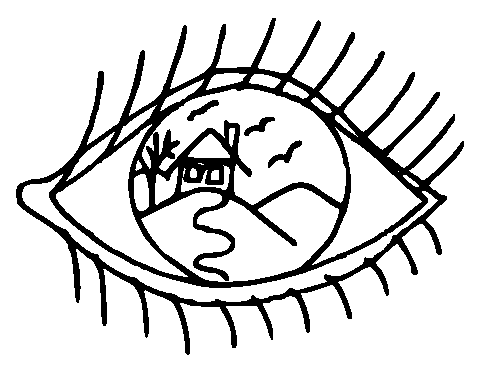
\includegraphics[width=10cm]{images/11.eps}
\vfil
\pagebreak
\begin{TEXT}{Vlak Boží}
\SLOKA Už \Ch{G}{při}jíždí vlak Boží, \NL
je \Ch{C}{sly}šet stále \Ch{D}{blíž} \NL
a \Ch{G}{rachot} \Ch{G7}{kol} jeho \Ch{C}{vozů} \Ch{A}{ }\NL
nese \Ch{G}{kraji}\Ch{D}{nou} se \Ch{G}{již.}
\REFREN  /: \Ch{G7}{Nu}že \Ch{C}{dál,} vstupte, děti milé, \Ch{G}{dál,} \NL
vstupte, děti milé, \Ch{C}{dál,} \NL
děti \Ch{A7}{milé,} zde \Ch{G}{každý} \Ch{D}{místo} své \Ch{G}{má.} :/
\SLOKA Já slyším, jak tam píská,\NL
když do zatáčky vjel\NL
a uhání plnou parou,\NL
jak by roztrhnout se chtěl.
\SLOKA Vstupte, jízda s ním je levná,\NL
jet každý může v něm,\NL
tam druhá třída není,\NL
ani rozdíl v cestovném.\NL
\end{TEXT}
 % 61
\begin{TEXT}{Vstoupí Mojžíš}
\REFREN  \Ch{e}{Vstoupí} \Ch{a}{Mojžíš} \Ch{H7}{do} země \Ch{e}{egypt}ské \NL
\Ch{e}{volá:} Fa\Ch{a}{rao,} \Ch{H7}{pusť} nás ze svých \Ch{e}{pout} 
\SLOKA Když \Ch{e}{Izra}\Ch{H7}{el žil} \Ch{e}{v otroc}\Ch{a}{tví,} \Ch{H7}{pusť} nás ze svých \Ch{e}{pout}\Ch{H7}{ } \NL
Už \Ch{e}{ne}moh' \Ch{H7}{snášet} \Ch{e}{útlak} \Ch{C7}{zlý,} \Ch{H7}{pusť} nás ze svých \Ch{e}{pout}\Ch{H7}{ }
\SLOKA Mojžíše s knězem Áronem… \NL
poslal Bůh za faraonem… 
\SLOKA Faraon na to neslyší… \NL
jen v robotách jim přitíží… 
\SLOKA Jen ten kdo málo práce má… \NL
na divné věci myslívá… 
\SLOKA Faraon pyšný nevěří… \NL
co všechno ještě udeří… 
\SLOKA Stane se posledního dne… \NL
co všem se zdálo nemožné… \NL
\end{TEXT}
 % 62
\pagebreak
\section{Zapadlo již slunce}
\begin{enumerate}
\item \Ch{e}{Zapadlo} již slun\Ch{C}{ce} \Ch{h}{všude} nastal \Ch{e}{klid} \\*
\Ch{G}{Jsme} však \Ch{C}{v Boží} \Ch{A h}{ruce} \Ch{G}{nepře}\Ch{D}{stal} Pán \Ch{e}{bdí}\Ch{A7}{t,} \\*\hspace*{5cm}\Ch{h}{nepřes}\Ch{F#}{tal Pán} \Ch{h}{bdít}
\item Dobrý pastýř Ježíš lidi miluje \\*
když se jemu svěříš /: světlo daruje :/ 
\item Temnot dlouhé noci nemusíš se bát \\*
ať máš ještě práci /: nebo ať jdeš spát :/ 
\item Až po noci temné nový svitne den \\*
chce být Ježíš věrně /: tebou oslaven :/ 
\item Jsme teď v Boží ruce když je všude klid \\*
Zapadlo již slunce /: nepřestal Pán bdít :/ \\*
\end{enumerate}
 % 63
  \pagebreak
\section{Žalm 150}
\begin{enumerate}
\item[Ref.:]  \Ch{(D)}{Hale}\Ch{G}{luja} chvalte Pána \\*
hale\Ch{a}{luja} \Ch{D7}{chvalte} \Ch{G}{Pána} \\*
hale\Ch{G7}{luja} chvalte \Ch{C}{Pána} \Ch{A7}{vším} \\*
\Ch{G}{chval} jej \Ch{D}{celá} \Ch{G}{zem} 
\item \Ch{(D)}{Chvalte} jej \Ch{G}{neboť} on je ten silný \\*
Chvalte jej \Ch{a}{neboť} on je ten \Ch{G}{mocný} \\*
Chvalte jej \Ch{G7}{neboť} \Ch{D7}{on} je ten \Ch{C}{svatý} \Ch{A7}{Pán,} \Ch{G}{ha}\Ch{D}{lelu}\Ch{G}{ja} 
\item Chvalte jej zvukem kytar a louten \\*
houslí a varhan \\*
chvalte jej neboť on je ten svatý Pán, haleluja 

\item Chvalte jej zvukem píšťal a bubnů \\*
trub a cymbálů \\*
chvalte jej neboť on je ten svatý Pán, haleluja 
\item Chvalte jej hlasem silným a zvučným \\*
chvalte jej každý, všechno co dýchá \\*
chvalte jej neboť on je ten svatý Pán, haleluja \\*
\end{enumerate}
 % 64
\pagebreak
\begin{TEXT}{Krásný je vzduch}
\SLOKA \hspace{0em}\rlap{/: \Ch{D}{Krásný} je \Ch{h}{vzduch} \Ch{e}{krásnější }je \Ch{A}{moře} :/} \hspace*{0.75\textwidth}\rlap{\Ch{E\,c#\,f#\,H}{ }} \NL
\hspace{0em}\rlap{/:\Ch{D}{co} je nejkrá\Ch{H7}{snější} \Ch{e}{co} je nejkrá\Ch{A}{snější} } \hspace*{0.75\textwidth}\rlap{\Ch{E\,C#\,f#\,H}{ }}\NL
\hspace{0em}\rlap{\Ch{D}{usmě}\Ch{A}{vavé} \Ch{D}{tváře} :/ } \hspace*{0.75\textwidth}\rlap{\Ch{E\,H\,E}{ }}
\SLOKA /:Pevný je stůl pevnější je hora:/ \NL
/:co je nejpevnější co je nejpevnější \NL
ta člověčí víra:/ 
\SLOKA /:Pustá je poušť i nebeské dálky:/ \NL
/:co je nejpustější co je nejpustější \NL
žít život bez lásky:/ 
\SLOKA /:Mocná je zbraň mocnější je právo:/ \NL
/:co je nejmocnější co je nejmocnější \NL
pravdomluvné slovo:/ 
\SLOKA /:Velká je zem šplouchá na ní voda:/ \NL
/:co je však největší co je však největší \NL
ta lidská svoboda:/ \NL
\end{TEXT}
 % 65
\vfil
\hspace*{2cm}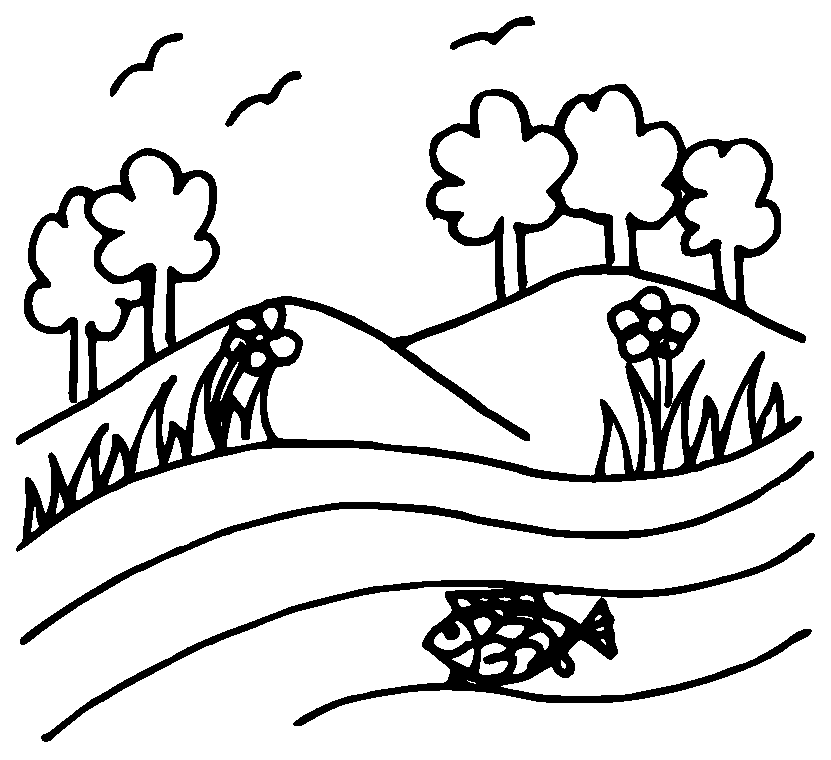
\includegraphics[width=10cm]{images/12.eps}
\vfil
\begin{TEXT}{Pocestný}
\SLOKA \Ch{A}{Je} to chůze \Ch{A7}{po} tom světě \Ch{D}{kam} se noha \Ch{A}{šine} \NL
/: \Ch{E}{sotva} \Ch{C#7}{přejdeš} \Ch{f#}{jedny} ho\Ch{D}{ry} \Ch{A}{hned} se naj\Ch{E}{dou} \Ch{A}{jiné} :/ 
\SLOKA Je to život na tom světě že by člověk utek \NL
/: ještě nezažil jsi jeden máš tu druhý smutek :/ 
\SLOKA Což je pánům ti ve voze sedí pěkně v suše \NL
/:ale chudý ten za nimi v dešti blátě kluše:/ 
\SLOKA Ej co já dbám na té cestě na psoty a sloty \NL
/: jen když já mám zdravé nohy k tomu dobré boty :/ 
\SLOKA Však na pány v krytém voze taky někdy trhne \NL
/: jednou se jim kolo zláme jindy vůz se zvrhne :/ 
\SLOKA A krom toho až své pouti přejedem a přejdem \NL
/: v jedné hospodě na nocleh pán nepán se sejdem :/ \NL
\end{TEXT}
 % 66
\vfil
\begin{TEXT}{Jednou budem dál}
\SLOKA \hspace{0em}\rlap{/: \Ch{A}{Jednou} \Ch{D}{budem} \Ch{A}{dál} :/ \Ch{f#}{ }} \hspace*{0.635\textwidth}\rlap{\Ch{C\,F\,C\,a}{ }}  \NL
\hspace{0em}\rlap{\Ch{A}{jednou} \Ch{D}{bu}\Ch{E}{dem} \Ch{f#}{dál,}\Ch{H7}{ já}\Ch{E}{ ví}\Ch{H7}{m,}\Ch{E7}{ ó,}\Ch{(DE)}{ }} \hspace*{0.635\textwidth}\rlap{\Ch{C\,F\,G\,a\,D7\,G\,D7\,G7\,(FG)}{ }}  \NL
\hspace{0em}\rlap{\Ch{A}{jen} \Ch{D}{víru} \Ch{A}{mít,} \Ch{D}{dou}\Ch{E}{fat} a \Ch{f#}{jít} } \hspace*{0.635\textwidth}\rlap{\Ch{C\,F\,C\,F\,G\,a}{ }} \NL
\hspace{0em}\rlap{\Ch{A}{jednou} \Ch{D}{budem} \Ch{A}{dál,} \Ch{E}{já} \Ch{A}{ví}\Ch{D}{m} \Ch{E}{ } } \hspace*{0.635\textwidth}\rlap{\Ch{C\,F\,C\,G\,C\,F\,G}{ }} 
\SLOKA Půjdem s druhem druh… 
\SLOKA Jednou přijde mír… 
\SLOKA Budem svobodni… 
\SLOKA Není proč se bát… 
\SLOKA Cíl je blízko nás… 
\SLOKA = 1.
\end{TEXT}
 % 67
\pagebreak
\begin{TEXT}{Starý příběh}
\SLOKA Řek' \Ch{D}{jednou} Mojžíš lidu svému přišel čas \NL
dnes v noci tiše \Ch{f#}{vytratí} se \Ch{G}{každý} \Ch{A}{z nás} \NL
\Ch{D}{má}v\Ch{D7}{á }\Ch{G}{má}\Ch{E}{vá} nám \Ch{D}{všem} svo\Ch{A}{bodná} \Ch{D}{zem}
\SLOKA Já říkám rovnou každý ať s tím počítá \NL
že naše cesta ke štěstí je trnitá \NL
mává mává nám všem svobodná zem 
\REFREN  /: \Ch{D}{Kdo} se bojí vodou jít \NL
ten podle tónu faraonů \Ch{E}{musí} \Ch{A}{žít} \NL
\Ch{D}{má}v\Ch{D7}{á }\Ch{G}{má}\Ch{E}{vá} nám \Ch{D}{všem} svo\Ch{G}{bodná} \Ch{D}{zem}  :/
\SLOKA Až první krůček bude jednou za námi \NL
tak nikdo nesmí zaváhat dát na fámy \NL
mává mává… 
\SLOKA Pak tenhle vandr všem potomkům ukáže \NL
že šanci má jen ten kdo má dost kuráže \NL
mává mává… 
\REFRENHRAJ
\SLOKA Ten \Ch{D}{sta}rý příběh \Ch{G}{z bi}ble vám tu \Ch{D}{vy}klá\Ch{G}{dám} \NL
ať \Ch{D}{}každý ví že \Ch{f#}{roz}hodnout se \Ch{G}{musí} \Ch{E}{sá}\Ch{A}{m} \NL
\Ch{D}{mává} mává… 
\end{TEXT}
 % 68
\vspace*{-1.8cm}\hspace*{6cm}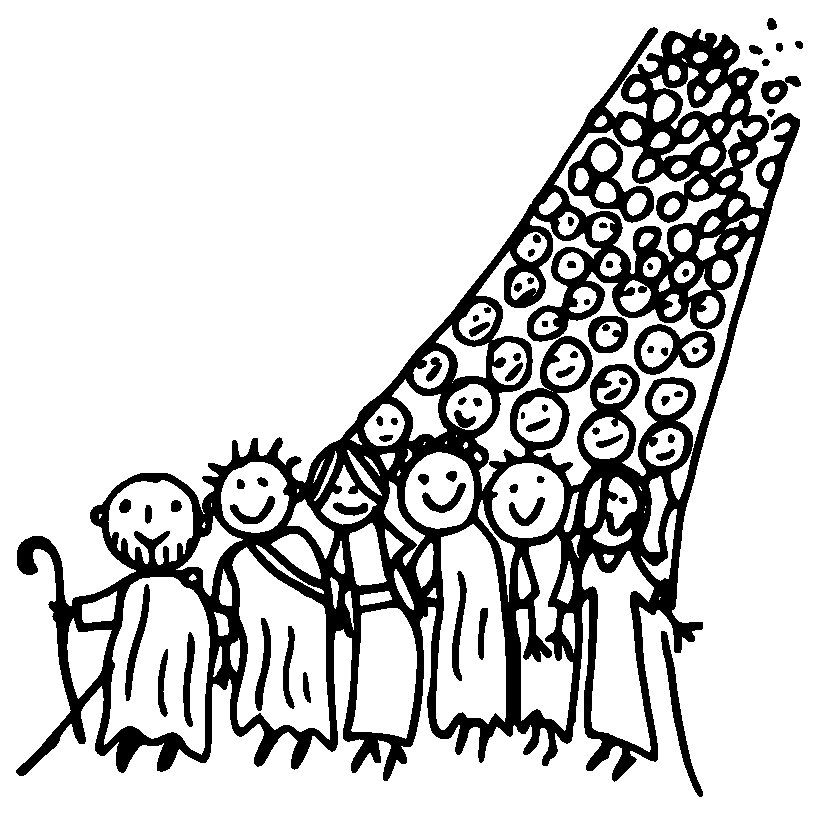
\includegraphics[width=5cm]{images/13.eps}
\begin{TEXT}{Kladivo}
\SLOKA Bylo by to \Ch{C}{krás}\Ch{a}{ný} \Ch{d}{bejt} \Ch{G}{bleskem} nebo \Ch{C}{bou}\Ch{a}{ří} \NL
\Ch{d}{bejt} \Ch{G}{vo}dou nebo \Ch{C}{trá}\Ch{a}{vou} \Ch{d}{bejt} větrem co \Ch{G}{vál} \NL
bejt kladivem v \Ch{a}{pěstích} bejt jiskřičkou v \Ch{F}{kou}\Ch{C}{ři} \NL
a kovadlinou \Ch{F}{bejt} a \Ch{C}{znít} a \Ch{F}{vocel}ově \Ch{C}{zvonit} \NL
\Ch{F}{ó} \Ch{C}{ } \Ch{G}{to} bych      si tak \Ch{C}{přál}  \Ch{a}{ } \Ch{d}{ } \Ch{G}{ } \Ch{C}{ } \Ch{a}{ } \Ch{d}{ } \Ch{G}{ }
\SLOKA Bylo by to krásný bejt zvonem kterej zpívá \NL
do nebe se dívá a nebo i dál \NL
zvoní že svítá anebo se stmívá \NL
bejt obyčejnej zvon a znít a vocelově zvonit \NL
ó to bych si tak přál 
\SLOKA Bylo by to krásný bejt v melodii tónem \NL
tím tónem kterej hladí jak hedvábnej šál \NL
tím tónem co ladí a zní pod balkónem \NL
bejt v melodii tón a znít a vocelově zvonit \NL
ó to bych si tak přál 
\SLOKA Bylo by to krásný bejt zvonem kterej zpívá \NL
i kladivem i tónem a bůhví čím dál \NL
a zpívat že svítá anebo se stmívá \NL
a zvučet jako zvon a znít a zpívat dobrým lidem \NL
ó to bych si tak přál \NL
\end{TEXT}
 % 69
\section{Ryl jen celej den ryl}
\begin{enumerate}
\item Já \Ch{a}{každý} ráno v sedm hodin vstal \\*
A \Ch{E7}{krumpáč} s lopatou vyfasoval \\*
Pak s \Ch{a}{partou} která makat dovede \\*
Jsem \Ch{E7}{došel} tam co tunel povede 
\item[Ref.:] \Ch{E7}{Já} /: \Ch{a}{ryl} jen \Ch{E7(G)}{celej} den \Ch{a}{ryl} :/ \\*
abych \Ch{F}{dřív} \Ch{G}{než} \Ch{C}{do} \Ch{G}{svý} \Ch{C}{boudy} pudu \Ch{E7}{spát} \\*
\Ch{a}{čaj} v kan\Ch{a/G}{týně} \Ch{a/F}{moh'} si \Ch{E7}{dát} \\*
já \Ch{a}{ryl} jen \Ch{E7}{celej} den \Ch{a}{ryl} \\*
celej den \Ch{E7}{jen} (jak \Ch{a}{krtek}) celej \Ch{E7}{den} jen \Ch{a}{ryl} 
\item Kdo netrhal skálu těžko pochopí \\*
co sám dynamit někdy natropí \\*
když jednou ráno došlo k vejbuchu \\*
Jim Goff vyletěl majli do vzduchu 
\item A když z tý vejšky zas na zem si kec' \\*
předák McCane ho popad' za límec \\*
Tak se mi zdá že línej jsi jak veš \\*
Mě ve vzduchu se flákat nebudeš 
\item Teď po létech když večer sedím sám \\*
na starý dobrý časy vzpomínám \\*
Zas slyším jak dole rány duněly \\*
když ve skalách jsem lámal tunely
\end{enumerate}
 % 70
\pagebreak
\vspace*{-1.3cm}\hspace*{6cm}
\includegraphics[height=3.5cm]{images/14.eps}\vspace*{-2.5cm}
\section{Jonatán}
\vfil
\begin{enumerate}
\item Když \Ch{G}{jaro} zaťukalo na dveře roku \Ch{C}{vosu}mnáctset\Ch{G}{šest} \\*
přišel \Ch{C}{vod} řeky chlap \Ch{G}{co} sem jel jen \Ch{a}{sám} a na svou \Ch{D}{pěst} \\*
na \Ch{G}{sobě} hrubej pytel vod kafe nosil \Ch{C}{místo} kabá\Ch{G}{tu} \\*
starý \Ch{C}{vosadníci} \Ch{G}{hádali} co k \Ch{a}{čertu} \Ch{D}{hledá} \Ch{G}{tu} 
\item[Ref.:] Byl \Ch{e}{vazoun} děsný síly co sto šedesát mílí se \\*
/: \Ch{G(e)}{proti} proudu dřel :/ \\*
kam \Ch{A}{šel} ho všude chválej že jabloňovou álej \\*
/: pro \Ch{G(D)}{všechny} vysázel :/ \Ch{G}{ } \Ch{C}{ } \Ch{D}{ } \Ch{G}{ }
\item Dva měchy který složil v kantýně přivez' na dvou kánoích \\*
a jak v lokálu svý jméno řek' v tu ránu kdekdo ztich \\*
tam u nás bylo sice nezvyklý ale každej časem znal \\*
Jonatána co k nám jablečný jadýrka vozíval 
\item Když léty unavenej do trávy se svez a na zem sed \\*
vopřel se svejma zádama vo strom co právě kvet \\*
my spát pak nechali ho na místě kde právě přestal žít \\*
krásnější pomník nešel by snad vůbec postavit 
\item Až jednou nebudete na světě lidi ať tu po vás maj' \\*
/: třeba jabka nebo písničku co si rádi zazpívaj' :/ 
\end{enumerate}
 % 71
\begin{TEXT}{Severní vítr}
\SLOKA Jdu \Ch{D}{s děravou} patou mám \Ch{h}{horečku} zlatou \NL
jsem \Ch{G}{chudý} jsem sláb nemo\Ch{A}{cen} \NL
a \Ch{D}{hlava} mě pálí a \Ch{h}{v modravé} dáli \NL
se \Ch{G}{leskne }a \Ch{A7}{třpytí} můj \Ch{D}{sen} \Ch{A7}{ }  
\SLOKA Kraj pod sněhem mlčí tam stopy jsou vlčí \NL
tam zbytečně budeš mi psát \NL
sám v dřevěné boudě sen o zlaté hroudě \NL
já nechám si tisíckrát zdát 
\REFREN  Severní \Ch{D7}{vítr} je \Ch{G}{krutý} \Ch{D}{počítej} lásko má \Ch{A}{s tím} \NL
\Ch{D}{k nohám} ti \Ch{D7}{dám} zlaté \Ch{G}{pruty} nebo se \Ch{D}{vůbec} \Ch{A7}{nevrá}\Ch{D}{tím} 
\SLOKA Už zarůstám vousem a vlci už jdou sem \NL
už slyším je výt blíž a blíž \NL
už mají mou stopu už větří že kopu \NL
si hrob a že stloukám si kříž 
\SLOKA Zde leží ten blázen chtěl dům a chtěl bazén \NL
a opustil tvou krásnou tvář \NL
mám plechovej hrnek v něm pár zlatejch zrnek \NL
a nad hrobem polární zář \NL
\end{TEXT}
 % 72
\hspace*{5cm}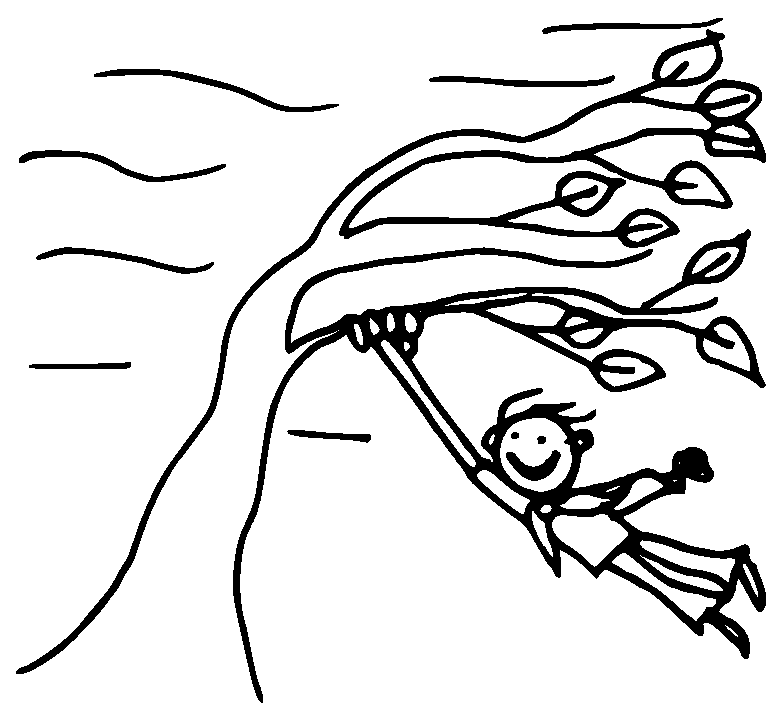
\includegraphics[width=6cm]{images/15.eps}
\begin{TEXT}{Není nutno}
\SLOKA \Ch{C}{Není} nutno není nutno aby bylo přímo vese\Ch{d}{lo} \NL
\Ch{G}{hlavně} nesmí býti smutno natož aby se breče\Ch{C}{lo} \Ch{G}{ } \NL
\Ch{C}{chceš}-li trap se že ti v kapse zlaté mince nechře\Ch{d}{stí} \NL
\Ch{G}{ne}mít žádné kamarády tomu já říkám neště\Ch{C}{stí} 
\REFREN  Nemít \Ch{a}{prachy} -- \Ch{e}{nevadí\,!!!} \NL
nemít \Ch{a}{srdce} -- \Ch{e}{vadí}\,!!! \NL
zažít \Ch{a}{krachy} -- \Ch{e}{nevadí}\,!!! \NL
zažít \Ch{a}{nudu} -- \Ch{F}{jóóó} to \Ch{G}{vadí}\,!!! \NL
\end{TEXT}
 % 73
\pagebreak
\begin{TEXT}{Mravenčí ukolébavka}
\SLOKA \Ch{D}{Slunce} šlo \Ch{A}{spát} za \Ch{D}{hromádku} \Ch{A}{klád} \NL
\Ch{D}{na} nebi \Ch{G}{hvězdy} klí\Ch{A}{čí} \NL
\Ch{D}{už} nepra\Ch{A}{cuj} \Ch{D}{mra}venečku \Ch{A}{můj} \NL
\Ch{D}{scho}vej \Ch{h}{se} \Ch{e}{do} je\Ch{A}{hli}\Ch{D}{čí} 
\REFREN  \Ch{D}{Máš} \Ch{e}{no}žičky \Ch{f#}{ubě}ha\Ch{A}{né} \Ch{D}{den} \Ch{G}{byl} tak těž\Ch{A}{ký} \NL
\Ch{D}{pojď} \Ch{e}{lů}žko máš \Ch{f#}{ode}stla\Ch{A}{né} \Ch{D}{v plátku} \Ch{A}{od} maceš\Ch{D}{ky} 
\SLOKA Usnul a sní mravenec lesní v hromádce u kapradí \NL
není tam sám s maminkou je tam \NL
tykadlama ho hladí. 
\end{TEXT}
 % 74
\vfil
\hspace*{1cm}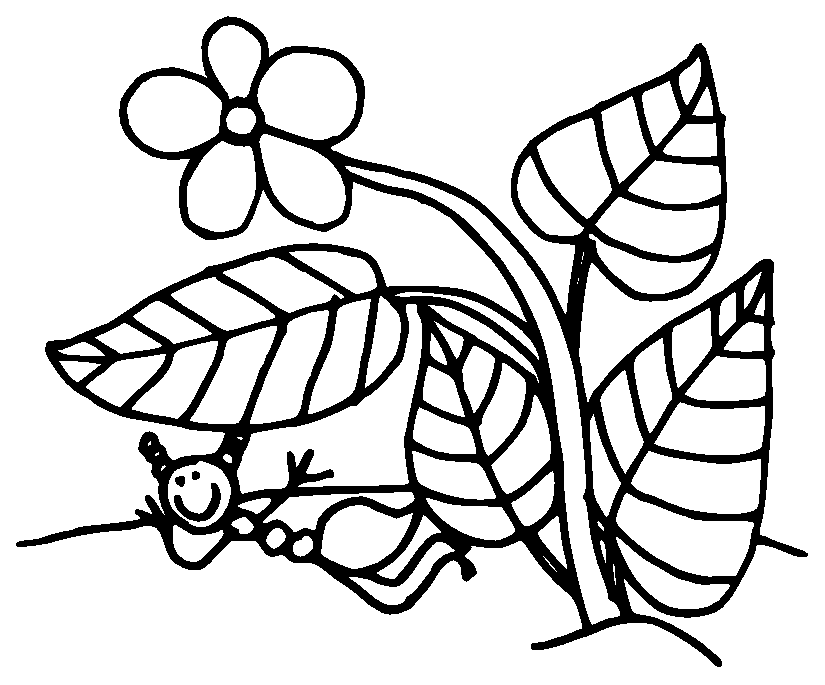
\includegraphics[width=11cm]{images/16.eps}
\vfil
\pagebreak
\section{Voláme sluníčko}
\begin{enumerate}
\item \Ch{D}{Voláme} sluníčko \Ch{G}{ha}\Ch{D}{ló,} \Ch{A}{ha}\Ch{D}{ló} \\*
tepla je na světě \Ch{A}{má}\Ch{D}{lo,} \Ch{G}{má}\Ch{D}{lo} \\*
vylez a rozežeň \Ch{G}{mra}\Ch{D}{ky,} \Ch{A}{mra}\Ch{D}{ky} \\*
a já ti pomůžu \Ch{A}{ta}\Ch{D}{ky, } \Ch{G}{ta}\Ch{D}{ky}  
\item Voláme skřivana /: haló :/ \\*
písní je na světě /: málo :/ \\*
přileť a zazpívej /: pro mě :/ \\*
žijeme přec v jednom domě 
\item Voláme človíčku /: haló :/ \\*
lásky je na světě /: \Ch{A}{má}\Ch{D}{lo}  \Ch{G}{má}\Ch{D}{lo} :/ 
\end{enumerate}
 % 75
\vfil
\hspace*{2cm}
\includegraphics[width=11cm]{images/17.eps}
\vfil
\pagebreak
\section{Hejna včel}
\begin{enumerate}
\item \Ch{a}{Nějak} umírá nám \Ch{a/G}{láska} \\*
my jako \Ch{a/F}{hejna} divejch \Ch{E}{včel} jdeme \Ch{a}{dál} \Ch{a/G}{ } \Ch{a/F}{ } \Ch{E}{ }
\item každej vztah je vlastně sázka \\*
každý ráno může zmizet                        my jdeme dál 
\item[Ref.:] \Ch{a}{Řekně}te kdopak za to \Ch{a/G}{může} \\*
kdo z nás má \Ch{a/F}{právo} něco br\Ch{E}{át } \\*
\Ch{a}{kdo} učil lidi zlobu \Ch{a/G}{dýchat} \\*
kdo na vo\Ch{a/F}{jáky} chce si \Ch{E}{hrát}
\item Už zase bohatejch je spousta \\*
a čím víc peněz lásky míň                    jdeme dál
\item A všichni plnou pusu slov \\*
že prý už zítra zítra snad                    budeme dál
\item[Ref.]
\item Už zase umírá nám láska \\*
my jako hejna divejch včel \\*
jdeme dál…
\end{enumerate}
 % 76
\pagebreak
\section{Strom} % NET
\begin{enumerate}
\item \Ch{a}{Polní} cestou kráčeli šuma\Ch{G}{ři} do vísky hrát \\*
\Ch{a}{svatby} pohřby tahle cesta po\Ch{G}{znala} tolikrát \\*
Po \Ch{F}{jedné} svatbě se \Ch{G}{chudým} lidem \Ch{C}{synek} naro\Ch{a}{dil} \\*
a \Ch{F}{táta} mu u \Ch{G}{prašný} cesty \Ch{E}{života} strom zasadil 
\item[Ref.:] A on tam \Ch{A}{stál} a koukal \Ch{f#}{do polí} \\*
byl jak \Ch{D}{král} sám v celém \Ch{E}{okolí} \\*
korunu \Ch{A}{měl}, korunu měl, i když ne \Ch{D}{ze} zlata  \\*
a jeho \Ch{A}{pokladem} byla \Ch{E}{tráva} střapa\Ch{A}{tá} 
\item Léta běží a na ten příběh už si nikdo nevzpomněl \\*
jen košatý strom se u cesty ve větru tiše chvěl \\*
a z vísky bylo město a to město začlo chtít \\*
asfaltovej koberec až na náměstí mít 
\item Že strom byl v cestě plánované to malý problém byl \\*
ostrou pilou se ten problém snadno vyřešil \\*
Tak naposled se náš strom do nebe podíval \\*
a tupou ránu do větvoví už snad ani nevnímal 
\item Při stavbě se ukázalo že silnice bude dál \\*
a tak kousek od nový cesty smutnej pařez stál \\*
Dětem ani výletníkům z výšky nikdo nemával \\*
jen přítel vítr si o něm píseň na strništi z nouze hrál 
\item[Ref.:] Jak tam stál… \\*
\end{enumerate}
 % 77
\begin{TEXT}{Franky dlouhán}
\SLOKA Kolik je \Ch{D}{smutného} když \Ch{G}{mraky} čer\Ch{D}{né} jdou \NL
lidem nad \Ch{A}{hlavou} \Ch{G}{smutnou} dála\Ch{D}{vou} \NL
Já slyšel příběh který \Ch{G}{velkou} pravdu \Ch{D}{měl} \NL
za čas odle\Ch{A}{těl} \Ch{G}{ } každý zapom\Ch{D}{něl} 
\REFREN  Měl kapsu \Ch{A}{prázdnou} Franky dlouhán \NL
po Státech \Ch{G}{toulal} se jen \Ch{D}{sám} \NL
a že byl \Ch{G}{veselej} tak \Ch{D}{každej} měl ho \Ch{A}{rád} \NL
Tam ruce \Ch{G}{k dílu} mlčky přiloží \NL
\Ch{D}{a zase} jede \Ch{h}{dál} \NL
a \Ch{G}{každej} kdo s ním \Ch{A}{chvilku} byl \NL
tak \Ch{G}{dlou}ho \Ch{A}{se} pak \Ch{D}{smál} 
\SLOKA Tam kde byl pláč tam Franky hezkou píseň měl \NL
slzy neměl rád chtěl se jenom smát \NL
A když pak večer ranče tiše usínaj' \NL
Frankův zpěv jde dál, nocí s písní dál 
\SLOKA Tak Frankyho vám jednou našli přestal žít \NL
jeho srdce spí tiše smutně spí \NL
Bůhví jak, za co tenhle smíšek konec měl \NL
farář píseň pěl umíráček zněl \NL
\end{TEXT}
 % 78
\section{Skautská večerka}
\begin{enumerate}
\item Zapad' den \\*
slunce svit vymizel z údolí z temen hor \\*
odpočiň každý kdos Boží tvor 
\item V lesa klín padl stín \\*
hasne již vatry zář svatý mír kráčí z hor \\*
usíná Boží tvor 
\item sloka brumendo \\*
\end{enumerate}
 % 82
\section{Zajíci}
\begin{enumerate}
\item \Ch{G}{Pod}zimní bílá mlha \Ch{C}{válí} se \Ch{G}{po} mechu \\*
\Ch{a}{myslivci} \Ch{D}{vstali} už \Ch{G}{ráno} \\*
\Ch{G}{Zajíci} zalezli a \Ch{C}{nechce} se jim z \Ch{G}{pelechu} \\*
\Ch{a}{neboť} se \Ch{D}{chtějí }dožít \Ch{G}{Vánoc} 
\item[Ref.:] \Ch{G}{Vzduchem} zní fanfára \Ch{D}{tramtará} rarara \\*
\Ch{C}{po} poli kráčejí \Ch{G}{střelci} \Ch{D}{ } \\*
\Ch{G}{Já} se svou \Ch{D}{kytarou} \Ch{C}{zpívám} písničku \Ch{G}{prastarou} \\*
\Ch{a}{o tom} že \Ch{D}{malí} budou \Ch{G}{velcí} \\*
Pam pam pam padada dam… \\*
Já se svou kytarou zpívám písničku prastarou \\*
o tom že malí budou velcí 
\item Zajíci naposledy potřesou si tlapkama \\*
a potom obléknou dresy \\*
Začíná specielní slalom mezi brokama \\*
na trati pole louky lesy 
\item Už volá vrchní zajíc Pravda vítězí \\*
nohy jsou naše hlavní zbraně \\*
až tu to skončí sraz je v sedm večer na mezi \\*
a teď zajíci hurá na ně 
\item[Ref.:] … pam pam pam… \\*
Já se svou kytarou zpívám písničku prastarou \\*
/: \Ch{a}{o tom} že \Ch{D}{malí} budou \Ch{G}{velcí} \Ch{e}{:/} \\*
\Ch{a}{že} všichni \Ch{D}{ma}lí budou \Ch{G}{ve}lcí 
\end{enumerate}
 % 80
\pagebreak
\begin{TEXT}{Doney Gal}
\SLOKA Kdo \Ch{D}{ví} proč to \Ch{A}{hříbě} tak \Ch{G}{v lás}ce \Ch{D}{mám} \NL
\Ch{D}{stádo} mu \Ch{A}{zblou}dilo \Ch{G}{bůh}ví \Ch{D}{kam} 
\REFREN  Ať \Ch{D}{sníh} či déšť padá tmou \NL
\Ch{A}{já} a můj \Ch{G}{Doney} Gal \Ch{D}{nesmí}\Ch{A}{me} \Ch{D}{snít} \NL
\Ch{D}{stále} dál cestou svou \NL
\Ch{A}{já} a můj \Ch{G}{Doney} Gal \Ch{D}{musí}\Ch{A}{me} \Ch{D}{jít} 
\SLOKA V zádech už máme snad tisíce mil \NL
stále jen spolu jdem neznáme cíl 
\SLOKA Až z \Ch{E}{nás} jeden \Ch{H}{zůstane} \Ch{A}{v klínu} \Ch{E}{hor} \NL
já ať to \Ch{H}{jsem} a ne \Ch{A}{můj} Doney \Ch{E}{Gal} \NL
\end{TEXT}
 % 79
\vfil
\hspace*{2cm}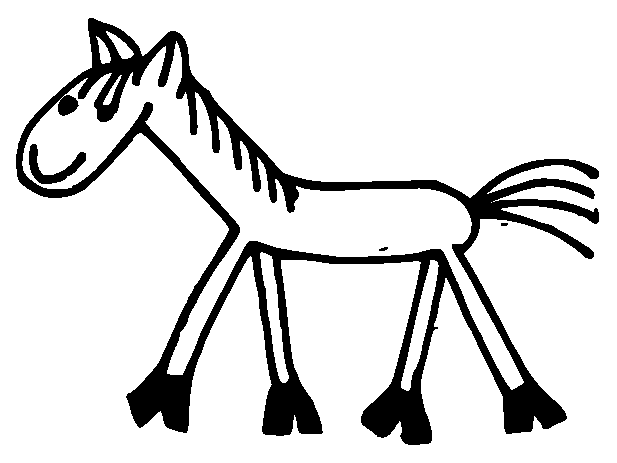
\includegraphics[width=7cm]{images/18.eps}
\vfil
\section{Dokud se zpívá} %net                                   \Ch{}{}
\begin{enumerate}
\item \Ch{C}{Z Tě}šína \Ch{e}{vyjíž}dí \Ch{d7}{vlaky} co \Ch{G}{čtvrt}hodi\Ch{C}{nu} \Ch{e}{ } \Ch{d7}{ } \Ch{G}{            } \\*
\Ch{C}{Včera} jsem \Ch{e}{nespal} a \Ch{d7}{ani} dnes \Ch{G}{ne}spoči\Ch{C}{nu } \Ch{e}{ } \Ch{d7}{ } \Ch{G}{        } \\*
\Ch{F}{svatý} Me\Ch{G}{dard} můj pat\Ch{C}{ron} ťuká si na če\Ch{G}{lo}  \\*
Ale: \Ch{F}{dokud} se \Ch{G}{zpívá} \Ch{F}{ještě} se \Ch{G}{neumře}\Ch{C}{lo} \Ch{e}{       } \Ch{d7}{ } \Ch{G}{ }
\item Ve stánku koupím si housku a slané tyčky \\*
srdce mám pro lásku a hlavu pro písničky \\*
ze školy dobře vím co by se dělat mělo \\*
Ale: dokud se zpívá ještě se neumřelo 
\item Do alba jízdenek lepím si další jednu \\*
vyjel jsem před chvílí konec je v nedohlednu \\*
za okny míhá se život jak leporelo \\*
Ale: dokud se zpívá ještě se neumřelo 
\item Stokrát jsem prohloupil a stokrát platil draze \\*
houpe to houpe to na housenkové dráze \\*
I kdyby supi se slítali na mé tělo \\*
dokud se zpívá ještě se neumřelo 
\item Z Těšína vyjíždí vlaky až na kraj světa \\*
Zvedl jsem telefon a ptám se Lidi jste tam? \\*
A z veliké dálky do uší mi zaznělo \\*
/: Dokud se zpívá ještě se neumřelo :/ \\*
\end{enumerate}
 % 81
\pagebreak
\begin{TEXT}{Hora Říp}
\REFREN  \Ch{G}{Už} je to dávno kroniky tvrdí \NL
\Ch{D}{tam} kde se tyčí hora Říp \NL
\Ch{A}{pár} lidí hledalo mléko a strdí \NL
\Ch{h}{zem} s vůní květů \Ch{G}{sta}letých \Ch{A}{lip} \NL
\Ch{G}{Kdy}koli z dálky vracíš se domů \NL
\Ch{D}{tak} jako tenkrát hledáš zas \NL
\Ch{A}{jak} dojít do země lipových stromů \NL
\Ch{h}{vždyť} jejich \Ch{G}{vů}ně \Ch{A}{zů}stala \Ch{D}{v nás} 
\SLOKA Dojít až \Ch{A}{tam} kde zrovna zraje \Ch{D}{réva} \NL
a člověk nena\Ch{A}{lévá} jen poloviční \Ch{D}{číš} \NL
dojít až \Ch{A}{tam} kde vyzvánějí \Ch{D}{k svá}tku \NL
a dětem pro po\Ch{A}{hádku} se v píseň promě\Ch{D}{níš} \NL
Na, \Ch{A}{na}, \Ch{D}{na}, \Ch{A}{na} \Ch{D}{…} 
\SLOKA Dojít až tam kde vlas babího léta \NL
všem stromům závoj splétá než uloží je spát \NL
dojít až tam kde písně kolovrátků \NL
ze starých bájí na památku \NL
všem lidem mohou hrát \NL
Na na na na… \NL
\end{TEXT}
 % 83
\begin{TEXT}{Pramínek vlasů}
\SLOKA \Ch{A7}{Když} měsíc \Ch{D}{rozli}je \Ch{h}{svě}tlo své \Ch{e}{po} kra\Ch{A7}{ji} \NL
a hvězdy \Ch{D}{řeknou,} \Ch{h}{že }čas je jít \Ch{e}{spát,} \Ch{A7}{ } \NL
pramínek \Ch{D}{vlasů}\Ch{h}{ jí} ustřihnu \Ch{e}{pota}jí. \Ch{A7}{ }\NL
Komu? No \Ch{D}{přece} té,\Ch{B(7)}{ kte}\Ch{A}{rou} mám \Ch{D}{rád.} \Ch{A7}{ } 
\SLOKA Pramínek vlasů jí ustřihnu potají, \NL
já blázen pod polštář chci si ho dát, \NL
ačkoliv sny se mi zásadně nezdají, \NL
věřím, že dnes v noci budou se zdát. 
\SLOKA O sny mě \Ch{C7}{připraví} teprve \Ch{D}{svítání,} \NL
zpěv ptáků \Ch{C7}{v oblacích} a modré \Ch{D}{nebe,} \NL
od vlasů, \Ch{f#}{jichž} jsem se dotýkal \Ch{H}{ve spaní,} \NL
nový den \Ch{G}{nůžkama} \Ch{B(7)}{odstřihne} \Ch{A7}{tebe.} 
\SLOKA Na bílém polštáři do kroužku stočený, \NL
zbude tu po tobě pramínek vlasů, \NL
já nebudu vstávat, dál chci ležet zasněný, \NL
/: je totiž \Ch{D}{neděl}\Ch{B(7)}{e a }\Ch{A7}{mám dost} \Ch{D}{ča}su :/ 
\end{TEXT}
 % 84
\begin{TEXT}{Končí divadlo}
\SLOKA \Ch{C}{Všechno} vždycky \Ch{G}{nějak} dopad\Ch{C}{lo} \NL
\Ch{F}{končí} den a \Ch{C}{končí} divad\Ch{G}{lo} \NL
/: \Ch{F}{můry} a \Ch{G}{noční} ptáci \NL
\Ch{C}{už} si šli \Ch{a}{hledat} práci \NL
\Ch{d}{a }slunce \Ch{G}{v }tůňce vychl\Ch{C}{adl}\Ch{C7}{o } :/
\SLOKA Sen o kouzelným verpánku \NL
vloudí se dětem do spánku \NL
Tmou temnou domů spěchám \NL
všem opuštěným střechám \NL
kočičí largo nechám hrát \NL
a ráno světlo denní \NL
mě v rámci probuzení \NL
donutí tiše zazpívat 
\SLOKA La la lala lala lalala… \NL
\end{TEXT}
 % 85
\vfil
\section{Škrhola}
\begin{enumerate}
\item \Ch{G}{V pimperlové} \Ch{D}{komedii} \Ch{G}{staló} se \Ch{G7}{ } \\*
\Ch{C}{Že }usedla vosa králi \Ch{G}{na }nóse \\*
\Ch{H7}{Král} se namích \Ch{E7}{a bóch} pěstí \Ch{A}{do} stólu: \Ch{Gdim}{ } \\*
\Ch{G}{Zavolejte} \Ch{D}{na tu} vosu \Ch{G}{Škrhólu.} 
\item Škrhola si řek že vosu prožéne \\*
Sukovicú mohutně se ožéne \\*
A jak tak ta vosa sedí na nóse \\*
Bóchne jí a v tu ránu je po vóse 
\item \Ch{C}{Zbývá} jen abychom \Ch{G}{k tomu} dodali \\*
že \Ch{D}{v tu} ránu \Ch{G}{je po} vose \Ch{C}{a po} krá\Ch{D}{li} 
\item Chtěl bych radit nijak vás však nenutím \\*
Malé věci řešte ruky mávnutím \\*
Nedopadnete tak jako Škrhola \\*
Nebudou vás považovat \\*
za císaře pána a jeho rodinu \\*
\end{enumerate}
 % 86
\pagebreak
\section{Kos}
\begin{enumerate}
\item Na tu \Ch{A6}{naši} zahradu \\*
\Ch{E}{Přiletěl} pták černej \\*
Podle \Ch{h}{mýho} odhadu \Ch{E}{ }\\*
\Ch{A6}{Byl} to asi kos 
\item \Ch{A6}{Když} mám dobrou náladu \\*
\Ch{E}{Bejvám} malichernej \\*
\Ch{h}{A proto} jsem za tím \Ch{E}{kosem} \\*
\Ch{A}{vyběh} \Ch{D}{z domu} \Ch{A}{bos} \Ch{E7}{ }  \\*
\Ch{A}{Chtěl} jsem vidět \Ch{E}{zblízka} \\*
\Ch{A}{jeho} černej \Ch{D}{frak} \\*
\Ch{A}{On} si ale \Ch{F#}{pískal} \\*
\Ch{h}{dopískal} \Ch{E}{a pak} 
\item \Ch{A}{Uletěl} mi \Ch{E}{z očí}  \Ch{A}{a já} zůstal \Ch{D}{sám} \\*
\Ch{A}{Země} se prej \Ch{F#}{točí} \Ch{h}{co} však z toho \Ch{E}{mám} \\*
\Ch{A}{Chybí} mi ta \Ch{E}{kosí}          \Ch{A}{píseň} \Ch{D}{veselá} \\*
/: \Ch{D}{která} doce\Ch{A}{la}  \Ch{E}{tiše} dozně\Ch{A6}{la} :/
\end{enumerate}
 % 87
\section{Marnivá sestřenice}
\begin{enumerate}
\item \Ch{C}{Měla} vlasy samou loknu, jé \Ch{G}{jeje} \\*
\Ch{G}{rán}o přistoupila k voknu, jé \Ch{C}{je} je \\*
\Ch{C}{vlasy} samou \Ch{C7}{loknu} měla \\*
/: \Ch{F(C)}{a na nic} víc \Ch{f(A)}{nemyslela} :/ \Ch{F}{jé}  \Ch{G}{jé} \Ch{C}{je} 
\item Nutno ještě podotknouti \\*
že si vlasy kulmou kroutí \\*
Nesuší si vlasy fénem \\*
/:nýbrž jen tak nad plamenem:/ 
\item Jednou vlasy sežehla si \\*
tím pádem je konec krásy \\*
Když přistoupí ráno k voknu \\*
/:nemá vlasy samou loknu:/ 
\item O vlasy už nestará se \\*
a diví se světa kráse \\*
Vidí plno jinejch věcí \\*
/:a to za to stojí přeci:/ \\*
\end{enumerate}
 % 89
\begin{TEXT}{Sádlo na chleba}
\SLOKA[] \Ch{A}{Sádlo} na chleba, \Ch{G#}{do vlasů }kvítí \NL
\Ch{A}{víc} už netřeba, \Ch{F#}{může} se jít \NL
\Ch{h}{Tam }kam půjdeme, \Ch{E}{mít} se budeme \NL
\Ch{A}{Jednou} zase \Ch{H}{báječně,} \Ch{E7}{jako} prase v žitě má se \NL
\Ch{A}{Víc} už netřeba, \Ch{G#}{může} se jíti \NL
\Ch{A}{Ba} i dareba \Ch{F#}{dovede} snít \NL
\Ch{h}{Že} život není \Ch{Adim}{pes} \NL
\Ch{A}{A že} nás láká \Ch{H}{les} \NL
\Ch{H}{V lese} je \Ch{E}{neděle}, \Ch{H}{chceme} zde \Ch{E}{vesele} \NL
\Ch{H}{na} duchu \Ch{E}{na} těle \Ch{A}{křát}. \NL
\end{TEXT}
 % 92
\pagebreak
\begin{TEXT}{Písnička o Davidovi}
\SLOKA \Ch{E}{K nebi} zvedal \Ch{A}{těžký} \Ch{E}{meč} \Ch{H}{každý} \Ch{F#}{se} ho \Ch{H}{bál} \NL
\Ch{E}{David} měl jen \Ch{A}{prak} a hůl \Ch{E}{Goli}\Ch{H7}{áš} se \Ch{E}{smál} \NL
\Ch{H}{Zpí}vejte s námi, \Ch{E}{zpí}vejte \Ch{A}{teď} \Ch{E}{s námi} \NL
\Ch{c#}{David} měl jen \Ch{f#}{prak} a hůl \Ch{E}{Goli}\Ch{H7}{áš} se \Ch{E}{smál} 
\SLOKA Však Bůh slabým pomáhá pyšné nemá rád \NL
proto David zvítězil obr k zemi pad' \NL
Zpívejte s námi, zpívejte teď s námi \NL
proto David zvítězil obr k zemi pad' 
\SLOKA Nedá pomoc meč a zbroj ale Pán Bůh náš \NL
Kdo mu věří silnější je než Goliáš \NL
Zpívejte s námi, zpívejte teď s námi \NL
kdo mu věří silnější je než Goliáš \NL
\end{TEXT}
 % 93
\begin{TEXT}{David a Goliáš}
\SLOKA* \Ch{C}{Lidi} na \Ch{a}{lidi} jsou jako \Ch{d}{sa}ně,\Ch{G7}{ } \Ch{C}{člověk} na člo\Ch{a}{věka} jako \Ch{G7}{kat} \NL
\Ch{C}{Podí}\Ch{C7}{vejte} \Ch{A}{se} na ně, \Ch{d}{musíte} \Ch{(A&)}{na}\Ch{G}{ří}\Ch{C}{kat} \Ch{H7}{ } \NL
\Ch{e}{Obr} do pidimužíka \Ch{H7}{mydlí,} \Ch{e}{domnívaje} se že vyhra\Ch{H7}{je} \NL
\Ch{G}{Klidně} \Ch{e}{seďme} \Ch{a}{na} žid\Ch{D7}{li,} \Ch{G}{čtěme} bibli \Ch{G7}{tam} to všechno je \NL
\Ch{C}{Samuelo}\Ch{a}{va} kniha nám \Ch{d}{poví}\Ch{G7}{dá,} \NL
\Ch{C}{jak} na Žida přišla veli\Ch{d}{ká} bí\Ch{G7}{da,} \NL
\Ch{C}{jak} ti bídní \Ch{C7}{Filištíni} \Ch{F}{válku} vést ne\Ch{f}{byli} líní \NL
\Ch{C}{až} potkali \Ch{A&7}{David}\Ch{G7}{a.}  \Ch{C}{David} šel do \Ch{a}{vá}lky volky, \Ch{d}{nevo}\Ch{G7}{lky,} \NL
\Ch{C}{z velké} dálky \Ch{a}{nesl} bratrům \Ch{d}{homo}\Ch{G7}{lky} \NL
\Ch{C}{v pochodu} se \Ch{C7}{cvičil} v hodu \Ch{F}{dal} si pro strýč\Ch{f}{ka} Příhodu \NL
\Ch{C}{tři} šutry do \Ch{A&}{to}\Ch{G}{bo}\Ch{C}{lky}  \NL
Hej \Ch{A&}{hej} kam se \Ch{C}{valej} vždyť jsou \Ch{D7}{malej} \NL
Takhle \Ch{G7}{Goliáš} ho \Ch{E7}{provokuje,} \Ch{d7}{David} slušně \Ch{G7}{salutuje} \NL
\Ch{C}{Když} mu ale \Ch{a}{obr} plivl \Ch{d}{do} oč\Ch{G}{í} \NL
\Ch{C}{David} se o\Ch{a}{to}čí prakem \Ch{d}{zato}\Ch{G7}{čí } \NL
\Ch{C}{Když} začínáš, \Ch{C7}{no} tak tumáš, \Ch{F}{byl} jsi velkej \Ch{f}{já} měl kuráž \NL
\Ch{C}{A jakej} byl \Ch{D7}{Go}\Ch{G7}{li}\Ch{C}{áš} 
\end{TEXT}
 % 94
\section{Bratry sestry potkávám} %net
\begin{enumerate}
\item Já \Ch{E}{vyšel} z města \Ch{G#}{v dálce} \Ch{C#}{za mnou} \\*
co \Ch{A}{měl} jsem rád jsem \Ch{C#}{opust}\Ch{f#}{il } \\*
a \Ch{A}{těším} \Ch{Edim}{se} že \Ch{E}{dojdu} \Ch{c#}{tam} \\*
kde \Ch{f#}{najdu} nový \Ch{H7}{pramen} \Ch{E}{sil} 
\item[Ref.:] \Ch{E}{ } Když bloudím \Ch{A}{ } pomoc \Ch{E}{čekám} \\*
a \Ch{A}{vím,} že nejsem \Ch{E}{sám} \\*
po \Ch{A}{úzký }\Ch{Edim}{cestě} \Ch{E}{da}lší \Ch{c#}{jdou} \\*
svý \Ch{f#}{bratry} sestry \Ch{H7}{potká}\Ch{E}{vám} 
\item Každej si to šlape po svejch nohách \\*
nemůže se s davem jenom vézt \\*
ale o to víc si můžou pomáhat \\*
a navzájem si břímě nést 
\item Netáhnu už s sebou žádnou z věcí \\*
co dřív jsem nutně musel mít \\*
stejně jenom těžký jsou \\*
a já už tam chci brzo být \\*
\end{enumerate}
 % 95
\pagebreak
\section{Šnečí blues}
\begin{enumerate}
\item \Ch{D}{Jednou} \Ch{G7}{jeden} \Ch{D}{šnek} \Ch{A}{ } \Ch{D}{šíle}\Ch{G}{ně} se \Ch{D}{lek',} \Ch{A7}{ } \\*
\Ch{D}{nikdo} už dnes \Ch{D7}{neví,} z \Ch{G}{čeho} se tak \Ch{g}{zjevil,} \\*
že se \Ch{D}{dal} hned \Ch{G7}{na} \Ch{A7}{ } \Ch{D}{útěk.} \Ch{A7}{ } 
\item Přes les a mýtinu rychlostí půl metru za hodinu, \\*
z ulity pára, ohnivá čára, \\*
měl cihlu na plynu. 
\item Ale v jedné zatáčce, tam v mechu u svlačce, \\*
udělal šnek chybu, nevyhnul se hřibu, \\*
nevyhnul se bouračce.
\item Hned seběhl se celý les a dali šneka pod pařez, \\*
tam v tom lesním stínu, jestli nezahynul, \\*
tak leží ještě dnes.
\item A kdyby použil vůz anebo autobus, \\*
/: nebylo by nutné zpívat tohle smutné, \\*
smutné šnečí blues. :/ 
\end{enumerate}
 % 96
\pagebreak
\section{To já ó Pane můj}
\begin{enumerate}
\item[Ref.:]  To \Ch{E}{já} ó \Ch{H7}{Pane} \Ch{E}{můj} \Ch{A}{půjdu} když mě \Ch{H7}{posí}\Ch{E}{láš } \\*
To \Ch{E}{já} ó \Ch{G#}{Pane} \Ch{c#}{můj} \Ch{A}{půjdu} když mě \Ch{H7}{posí}\Ch{E}{láš }
\item Koho pošlu kdo se hlásí je tu \Ch{H7}{cesta} \Ch{E}{má} \\*
\Ch{A}{půjdu} když mě \Ch{H7}{posí}\Ch{E}{láš} \\*
\Ch{E}{chceš} jít se mnou strach ti brání dát i \Ch{H7}{kůži} \Ch{E}{svou} \\*
\Ch{A}{půjdu} když mě \Ch{H7}{posí}\Ch{E}{láš.} 
\item K svému knězi k svému vládci a tak půjdu já \\*
půjdu když mě posíláš \\*
k těm co soudí co vše vědí a tak půjdu já \\*
půjdu když mě posíláš 
\item K těm co myslí že jsi mrtev a tak půjdu já \\*
půjdu když mě posíláš \\*
k těm co tvoří tvoji církev a tak půjdu já \\*
půjdu když mě posíláš \\*
\end{enumerate}
 % 97
\pagebreak
\begin{TEXT}{Krajina posedlá tmou}
\SLOKA \Ch{E}{Krajina} posedlá tmou \Ch{A}{ } \Ch{E}{ } \NL
\Ch{E}{vzpomínky} do sedla zvou \Ch{A}{ } \Ch{E}{  }  \NL
Nutí mě vrátit se \Ch{H}{tam} \Ch{A}{ } \Ch{H}{ }  \NL
kde budu na věky sám \Ch{A}{ } \Ch{H}{ } \NL
Kde místo úsměvů \Ch{E}{tvých,}\Ch{G#}{ } čeká jen řada snů \Ch{c#}{zlých} \NL
\Ch{A}{a místo} lásky nás \Ch{E}{dvou} \Ch{A}{ } \Ch{E}{ } krajina \Ch{H7}{posedlá} \Ch{E}{tmou.} \Ch{A E}{ }
\SLOKA Když západ v očích ti plál, \NL
s tebou jsem naposled stál, \NL
i když jsi čekala víc, \NL
přijel jsem tenkrát ti říct, \NL
že mám tě, na každej pád, jedinou na světě rád, \NL
a pak jsem zase jel dál a západ v očích ti plál. 
\SLOKA Proč jsem se vracel tak rád, \NL
proč jsem měl touhu se smát, \NL
když cestou řekli mi: Joe, ta nikdy nebude tvou. \NL
/: Že láska mizí jak dým, to dneska proklatě vím, \NL
jedno však musím se ptát, \NL
proč jsem se vracel tak rád. :/ \NL
\end{TEXT}
 % 98
\begin{TEXT}{Haú bílou plání}
\REFREN  \Ch{a}{Haú} bílou plání věčnou pusti\Ch{G}{nou} \NL
\Ch{a}{Letí} řada sání vlci v \Ch{H7}{patách} jim \Ch{E}{jsou} \Ch{E7}{ } \NL
\Ch{a}{Haú} kdo se zpozdí toho dosta\Ch{D}{nou} \NL
\Ch{e}{Jen} pár bílejch \Ch{d}{kostí} \Ch{a}{sně}\Ch{d}{hy} \Ch{a}{za}\Ch{E7}{van}\Ch{a}{ou} \Ch{G}{}
\INTERM Recitace: \NL
A: K \Ch{(C)}{snídani} je kousek mrože \NL
B: Cože? \NL
A: Mrože. \NL
B: Mrože? \NL
A: Bóže\,! \NL
B: K \Ch{C#}{obědu} dvě suchý tresky. \NL
A: To je hezký\,! \NL
B: Třesky plesky. \NL
A: \Ch{D}{Zato} k večeři nic není. \NL
B: \Ch{D#}{To} je pěkný nadělení. \NL
A: \Ch{E}{Proto} sníme \NL
B: \Ch{F#}{prot}o sníme \NL
A: \Ch{G}{proto} sníme \NL
B: proto sníme \NL
Všichni: /: \Ch{E}{psí} spře\Ch{E7}{žení} :/           4x \NL
\end{TEXT}
 % 99
\pagebreak
\newevenside
\begin{TEXT}{Nejsi sám svůj}
\SLOKA	\Ch{E}{Když} ti schází odvaha, \Ch{A7}{je} tu Ten, kdo pomáhá,\NL
	/: \Ch{H7}{nejsi} \Ch{EAE}{sám :/} \Ch{H7}{sám} \Ch{E}{svůj,} \Ch{A}{sám} \Ch{E}{svůj.}\NL
	Já vím, \Ch{E7}{já} vím, nejsem \Ch{A}{sám,} sám \Ch{EAE}{svůj,} \NL
	\Ch{H7}{Páně} \Ch{EAE}{jsem,} \Ch{A}{nejsem} \Ch{E}{sá}\Ch{A}{m}\Ch{E}{,} \Ch{H7}{sám} \Ch{E}{svůj,} \Ch{A}{sám} \Ch{E}{sv}\Ch{A}{ůj}. \Ch{E}{}
\SLOKA	Když tě pýcha zachvátí,je tu Ten, kdo říká ti:\NL
	Nejsi sám…
\SLOKA	Když jsi spoután řetězy, je tu Ten, kdo vítězí.\NL
	Nejsi sám…
\SLOKA	Když sis rakev přichystal, je tu Ten, kdo z mrtvých vstal.\NL
	Nejsi sám…
\end{TEXT}
 % 103
\pagebreak
\begin{TEXT}{Neboj se}
\SLOKA	Když \Ch{A}{bou}ře zuří zlá,\NL
  	když \Ch{D}{na}děj zemdlí\Ch{A}{vá,}\NL
	přec \Ch{E}{ne}musíš se bát,\NL
	přec \Ch{A}{ne}mu\Ch{D}{síš} se \Ch{A}{bát.}
\REFREN  	On ti \Ch{A}{pra}ví: \uv{S tebou jsem\,!}\NL
	On ti \Ch{D}{pra}ví: \uv{Neboj \Ch{A}{se\,!}}\NL
	On ti \Ch{h}{pra}ví: \uv{Můj jsi ty\,!}\NL
	praví: \uv{\Ch{A}{Můj} \Ch{D}{jsi} \Ch{A}{ty\,!}}
\SLOKA	Když jít máš přes vody\NL
	a nikde opory,\NL
	přec nemusíš se bát,\NL
	přec nemusíš se bát.
\REFRENHRAJ

\SLOKA	Když ohněm projít máš\NL
	a ochrany nemáš,\NL
	přec nemusíš se bát,\NL
	přec nemusíš se bát.
\REFRENHRAJ
\end{TEXT}
 % 104
\section{Stále jen chceme zpívat}
\begin{enumerate}
\item[Ref.:]	\Ch{G7}{Stá}le \Ch{C}{jen} chceme zpívat, \\*
	stále \Ch{G}{jen} chceme zpívat, \\*
	stále \Ch{C}{jen} chceme z\Ch{A7}{pívat,}\\*
	že \Ch{G}{Pán} zde \Ch{D}{mezi} námi \Ch{G}{je.}
\item	My \Ch{G}{často} vzdálili \Ch{G7}{se} \\*
	a \Ch{C}{nechali} jej \Ch{G}{stát,}\\*
	on \Ch{G}{přesto} \Ch{G7}{vždy} se \Ch{C}{vrací,} \Ch{A}{}\\*
	je \Ch{G}{me}zi \Ch{D}{ná}mi \Ch{G}{rád.} 
\item[Ref.]

\item	On nestaví si domy,\\*
	zámek jej nestřeží,\\*
	když k sobě lásku máme,\\*
	jsme jeho přístřeší. 
\item[Ref.]

\item	Udeřte slavně v bubny,\\*
	zpívejte, kdo jste kde,\\*
	do dlaní zatleskejte,\\*
	volejte Pán je zde\,! 
\item[Ref.] 
\end{enumerate}
 % 105
\section{Zpívej Pánu Haleluja}
\begin{enumerate}
\item[angl:]	\Ch{h}{Sing} hale\Ch{f#}{lujah} to the \Ch{h}{Lord,} \Ch{f#}{}\\*
	\Ch{h}{sing} hale\Ch{A}{lujah} to the \Ch{F#}{Lord}\\*
	\Ch{h}{sing} hale\Ch{A}{lujah,} \Ch{G}{sing} hale\Ch{D}{lu}jah\\*
	\Ch{h}{sing} hale\Ch{f#}{lujah} to the \Ch{h}{Lord.} \Ch{f#}{}

\item	Zpívej Pánu haleluja,\\*
	zpívej Pánu haleluja,\\*
	zpívej haleluja, zpívej haleluja,\\*
	zpívej Pánu haleluja .

\item	Ježíš je všeho světa Pán,\\*
	Ježíš je všeho světa Pán,\\*
	Ježíš je světa Pán, Ježíš je světa Pán,	\\*
	Ježíš je všeho světa Pán.

\item	Zvedněte k Pánu ruce své,\\*
	zvedněte k Pánu ruce své,\\*
	zvedněte ruce své, zvedněte ruce své,\\*
	zvedněte k Pánu ruce své.

\end{enumerate}
 % 106
\vfil
\begin{TEXT}{Kristus Pán}
\SLOKA	\Ch{C}{Do} kostela v \Ch{G}{džínách} občas \Ch{d}{chodí} Kristus \Ch{a}{Pán,}\NL
	\Ch{C}{do} copánku \Ch{G}{vlasy} občas \Ch{d}{nosí} Kristus \Ch{a}{Pán,} \NL
	\Ch{F}{v zimě} obut \Ch{G}{do} důchodek, \Ch{C}{v létě} v kristus\Ch{a}{kách,} \NL
	\Ch{d}{pře}kračuje \Ch{d7}{jist}ejch představ \Ch{G}{práh.}

\SLOKA	Denně scvrklou kůži oblíká si Kristus Pán,\NL
	po chodbách se vleče o dvou holích Kristus Pán.\NL
	Má v domově důchodců vše, co si může přát, \NL
	jak rád by měl navíc ještě rád.

\SLOKA	U běžících pásů taky sedá Kristus Pán,\NL
	do podzemních šachet taky fárá Kristus Pán,\NL
	koncem roku kvapem honí ohroženej plán, \NL
	upocenej dělník Kristus Pán.

\SLOKA	Na vysoký skály moc rád leze Kristus Pán,\NL
	pod širákem spává s partou trampů Kristus Pán,\NL
	záda rovný od usárny, šlape bláto cest,\NL
	dobře ví, kam každá musí vést.

\SLOKA	Poštu lidem nosí ve svý brašně Kristus Pán,\NL
	a ve vlacích lístky chodí štípat Kristus Pán, \NL
	a v moderně zařízenejch školních učebnách\NL
	od katedry hází na zeď hrách.

\SLOKA	Na saních rád jezdí jako vítr Kristus Pán,\NL
	na zamrzlý řece je vždy doma Kristus Pán,\NL
	dokáže si s vločkou sněhu na co chcete hrát,\NL
	dítětem se stává obzvlášť rád.
\end{TEXT}
 % 107
\begin{TEXT}{Ať dobrý Bůh}
\SLOKA	\Ch{D}{Ať} \Ch{e}{do}\Ch{f#}{brý} \Ch{G}{Bůh} je stále \Ch{A}{s vámi}, život \Ch{f#}{váš} ať promě\Ch{h}{ní,} \NL
	spoko\Ch{e}{jí} srdce \Ch{A}{vaše,} pokoj \Ch{D}{dá,} \Ch{D7}{} \NL
	\Ch{D}{ať} \Ch{e}{do}\Ch{f#}{brý} \Ch{G}{Bůh} je stále \Ch{A}{s vámi}, všechno \Ch{f#}{zlé}  ať přemá\Ch{h}{há,} \NL
	mezi \Ch{e}{vámi} mír a \Ch{A}{lásku} rozdá\Ch{D}{vá.}\Ch{D}{ } \Ch{e}{ } \Ch{f#}{ }

\REFREN 	\Ch{G}{S lás}\Ch{A}{kou,} ó s \Ch{f#}{lás}\Ch{h}{kou} \Ch{e}{sám} Je\Ch{A}{žíš} jde k \Ch{D}{nám.} \Ch{D}{ } \Ch{e}{ } \Ch{f#}{ }\NL
\Ch{G}{S lás}\Ch{A}{kou,} ó s \Ch{f#}{lás}\Ch{h}{kou} \Ch{e}{sám} Je\Ch{A}{žíš} jde k \Ch{D}{nám.} 

\SLOKA	Otvírá brány všem vězněným, všechna pouta přemáhá,\NL
	kde byl pláč, tam slzy smutku otírá.\NL
	Do říše Tmy a temných stínů přichází a svítí nám,\NL
	v jeho jménu nový život začíná.
\end{TEXT}
 % 108
\vfil
\begin{TEXT}{Vzdám celým srdcem svým}
\SLOKA \Ch{D}{Vzdám} \Ch{A}{ce}lým srdcem \Ch{h}{svým} Tobě \Ch{G}{chvá}\Ch{A}{lu} a \Ch{D}{dík,}\Ch{D7}{ }\NL
řeknu \Ch{G}{všem} o \Ch{A}{díle}, \Ch{F#}{které’s} uči\Ch{h}{nil,} budu \Ch{G}{zpí}\Ch{D}{vat} \Ch{e}{Tvé}mu \Ch{E7}{jmé}\Ch{A}{nu.}\NL
\Ch{D}{Vzdám} \Ch{A}{celým} srdcem \Ch{h}{svým} Tobě \Ch{G}{chvá}\Ch{A}{lu} a \Ch{D}{dík.} \Ch{D7}{ } \NL
Teď \Ch{G}{mám} jen \Ch{A}{v Pánu} \Ch{F#}{zdroj} své rado\Ch{h}{sti,} proto \Ch{G}{ha}\Ch{D}{le}\Ch{A}{lu}\Ch{D}{ja.}
\end{TEXT}
 % 109
\section{Můj Bůh je můj štít}
/: Můj  \Ch{D}{Bůh} je můj  \Ch{C}{štít}, je mou  \Ch{G}{písní}, já  \Ch{D}{vím.} \\*
On mi odpo\Ch{C}{ví,} mocí svého  \Ch{G}{jmé}na vysvobo\Ch{D}{dí.}\\*
Chci  \Ch{C}{žít} ve  \Ch{G}{stínu} křídel  \Ch{D}{Tvých,} \\* 
spě\Ch{C}{chám} do  \Ch{G}{stínu} křídel  \Ch{D}{Tvých,}\\*
smím  \Ch{C}{žít} ve  \Ch{G}{stínu} křídel  \Ch{D}{Tvých.}\\*
Teď  \Ch{D}{smím} jít v pokoji  \Ch{C}{dál,} vím, že jsi mi  \Ch{G}{blí}zko, \VOLTA[1]{halel\Ch{D}{uj}a} / \VOLTA[2]{am\Ch{D}{en}}. :/

 % 110
\pagebreak
\begin{TEXT}{Babylon}
\SLOKA \Ch{h}{Ten} obraz zlatý, \Ch{C}{obraz} se k nebi tyčí,\NL
\Ch{h}{zář} oči oslepí, \Ch{E}{zář} jeho oči ničí \NL
\Ch{h}{do} snů se vkrádá, \Ch{C}{vrývá} se do paměti,\NL
\Ch{h}{Babylon} hold si vzdává, \Ch{D}{Babylon} \Ch{F#}{sebe} světí.
\REFREN  \Ch{h}{Ač} z pece ohnivé \Ch{E}{žár} stoupá žhavý \NL
\Ch{h}{a obraz} zlatý \Ch{G}{dotýká} se \Ch{D}{hvězd,}\NL
Ho\Ch{a6}{spodin} \Ch{H7}{zástupů} je králem \Ch{e}{slávy,}\NL
\Ch{C}{jen} Bohu \Ch{G}{samému} \Ch{C}{vzdá}\Ch{D}{váme} \Ch{G}{čest.}

\SLOKA Tympány, housle, hudby, zpěv v jednom tónu,\NL
cimbály, pozouny, klaňte se Babylonu,\NL
ať lidská srdce v jediném rytmu buší,\NL
Babylon poctu žádá, Babylon žádá duši.
\REFRENHRAJ
\SLOKA Babylon dává poslední příležitost,\NL
vyjimky z pravidla, máte čas doznat lítost,\NL
teď cesta zpátky ještě je otevřena, \NL
uznejte vládu sochy, padněte na kolena.
\REFRENHRAJ
\end{TEXT}
 % 114
\begin{TEXT}{Svítá novej den}
\SLOKA* \Ch{d}{Sví}\Ch{a}{tá }\Ch{G}{novej} \Ch{a}{den} \Ch{d}{sví}\Ch{a}{tá }\Ch{G}{den.}
\SLOKA Je \Ch{a}{v sutinách město,} je \Ch{C}{zbořenej} \Ch{D}{chrám,}\NL
je \Ch{e}{zdrcený} ticho a tmy vládnou \Ch{a}{tmám.}\NL
V tom paprskem jitřním, \Ch{C}{slune}\Ch{D}{čním,}\NL
za\Ch{e}{lesk} se střep, co z rozvalin \Ch{a}{ční.}\NL
\REFREN  /: \Ch{d}{Sví}\Ch{a}{tá }\Ch{G}{novej} \Ch{a}{den} \Ch{d}{sví}\Ch{a}{tá }\Ch{G}{den,}:/
\SLOKA Pad vichřicí strom, ptáci vypadli z hnízd,\NL
slyšíš jejich křik, nemaj si kam vlízt.\NL
Vtom v kořenech starých pupen prask,\NL
hle, zelenej proutek, kde prach čekals.  
\REFREN \,
\SLOKA Poutník, co šel cestou, hložím podél skal,\NL
teď leh a spí, neví kudy dál.\NL
Vtom hlas tichý, temný zašeptal:\NL
Jen vstaň a pojď…   
\REFREN \,
\end{TEXT}
 % 116
\pagebreak
\begin{TEXT}{Tři mládenci}
\SLOKA \Ch{E}{Byli} tři mládenci co měli svůj styl\NL
\Ch{A}{měli} svou cestu a \Ch{E}{měli} svůj cíl\NL
\Ch{A}{měli} svou víru a \Ch{E}{byli} šik\NL
\Ch{F#}{ten} kdo je neznal \Ch{H}{těžko} si zvyk\NL
\Ch{E}{Sidrach} \Ch{A}{Mizach}  \Ch{H}{Abdenágo}
\SLOKA Byl jeden císařpán ten svátek měl\NL
aby mu zpívali a tančili chtěl\NL
a tak dle příkazu jásali lidi\NL
a ten kdo nejásal byli tři Židi\NL
Sidrach Mizach Abdenágo
\SLOKA Povídá císařpán mládenci zlatí\NL
i pro vás tahleta vyhláška platí\NL
dokažte jak každej z vás mě má rád\NL
budete tancovat a ne sa vykrůcat\NL
Sidrach Mizach Abdenágo
\SLOKA Váženej pantáto mládenci dí\NL
tancovat nebudem, do háje jdi\NL
zpívat ti nechceme pro nás jsi vzduch\NL
nad náma má moc jedině Bůh\NL
Sidrach Mizach Abdenágo
\SLOKA Císař se namích a na tohle vece\NL
strčte ty hošany do ohnivý pece\NL
plakati budou a křičeti: Ach!\NL
prach byli tak ať se obrátěj v prach\NL
Sidrach Mizach Abdenágo
\SLOKA Hořelo dříví a v peci byl hic\NL
ti tři mládenci se nebáli nic\NL
víra je lepší než kvádro z azbestu\NL
Hospodin svítil jim sirkama na cestu\NL
Sidrach Mizach Abdenágo
\SLOKA Tohle svět neviděl povídá král\NL
a jejich boha abych se bál\NL
kdybych jim ublížil byl by moc zlej\NL
tak ať si ksakru dělaj co chtěj\NL
Sidrach Mizach Abdenágo
\end{TEXT}
 % 115
\pagebreak
\begin{TEXT}{Balada velkopáteční}
\SLOKA \Ch{a}{Shromáždil} \Ch{E}{člověk} prý \Ch{C}{moudrosti} své \Ch{D}{poklad}\NL
\Ch{F}{uložil} jej \Ch{G}{do svých} příslo\Ch{a}{ví}\Ch{E}{}\NL
\Ch{a}{A kdo} chce \Ch{E}{pravdu} snad \Ch{C}{o životě} \Ch{D}{poznat}\NL
\Ch{F}{k tomu} ať ten \Ch{G}{poklad} promlu\Ch{a}{ví}\Ch{E}{}\NL
\Ch{A}{Chcete-li} však \Ch{A7}{takto} dojít \Ch{d}{poučení}\NL
\Ch{G}{nezůstaňte} v půli cesty \Ch{C}{stát}\Ch{E}{}\NL
\Ch{a}{Snažte} se \Ch{E}{naslouchat} \Ch{C}{jen} plnému \Ch{D}{znění}\NL
\Ch{F}{půlka} pravdy \Ch{G}{může} taky \Ch{a}{lhát}

\SLOKA Do jámy upadne kdo jiným ji chystá\NL
sejde mečem kdo s ním zachází\NL
Pravda však bývá pouze tehdy jistá\NL
když jí jedna půlka neschází\NL
Slyšte proto všichni druhou polovinu\NL
je v ní skryta moudrost odvěká:\NL
/: Ten kdo meč odmítá ten na kříži sejde\NL
slyšte lidé moudrost člověka :/
\end{TEXT} %121
\begin{TEXT}{Píseň proti trudnomyslnosti\\*(hymna~2008)}
\SLOKA* \Ch{D}{Polární} noc má zvláštní moc \NL
Každého přepadne smu\Ch{A7}{tek} \NL
Němec i Brit křesťan i žid \NL
Každý by nejradši u\Ch{D}{tek'} \NL
Ba i ti \Ch{G}{šiko}vní Žapon\Ch{D}{ci} \NL
Se sila\Ch{E}{mi} jsou na kon\Ch{A}{ci} \NL
Jen jeden z \Ch{D}{náro}dů nesko\Ch{G}{ná} \NL
Hrůzy \Ch{D}{Seve}ru \Ch{A}{sla}vně překo\Ch{D}{ná} 
\SLOKA* /: \Ch{D(A)}{Tam kde} hy- tam kde hy- kde hynuli \Ch{A(D)}{vlci} :/ \NL
Tam kde hy- tam kde hy- kde hynuli so\Ch{G}{bi} \NL
\Ch{A}{Čech} se přizpůso\Ch{D}{bí,} \Ch{A}{Čech} se přizpůso\Ch{D}{bí} \Ch{A}{ } \Ch{D}{ }\NL
\end{TEXT}
 % 100
\begin{TEXT}{Ahoj slunko}
\SLOKA \Ch{C}{Ahoj} \Ch{F}{ahoj} \Ch{C}{slunko}\NL
\Ch{Fdim}{tobě to teda dneska} \Ch{a7}{sekne}\NL
\Ch{d7}{včera} mi bylo \Ch{G}{smutno}\NL
ale \Ch{C}{dneska} už je \Ch{C/H}{zase} mírně \Ch{a7}{pěkně}\NL
\Ch{d7}{jó někdy} se \Ch{G}{zdá}\NL
že něco \Ch{C}{nejde} ale \Ch{C/H}{ono to pak} \Ch{a7}{jde}\NL
\Ch{d7}{doba} ta není \Ch{G}{zlá}\NL
to jenom \Ch{F}{některé} \Ch{G}{vteřiny} jsou \Ch{C}{zlé}

\SLOKA Ahoj ahoj slunko\NL
jsem rád že jsi ještě\NL
osuš mi moje vlasy\NL
jsou promáčené předvčerejším deštěm\NL
no prostě jsem zmok´\NL
naštěstí voda teče vždycky shora dolů\NL
už kolikátý rok\NL
to takhle přes překážky táhnem spolu

\SLOKA Ahoj ahoj slunko\NL
jsem rád že tě vidím\NL
doma mi bylo smutno\NL
a tak jsem zase vyšel mezi lidi\NL
srdce potřebuje svý\NL
a kdo bere měl by taky občas dát\NL
člověk ten není zlý\NL
jen prostě některé lidi nemám rád

\SLOKA Ahoj ahoj slunko\NL
ty máš dneska hezké tváře\NL
a kdyby mělo být snad smutno\NL
tak na to já mám svoje opraváře\NL
a tak dál mi sviť\NL
a až zalezeš za mraky jako tečka\NL
vylezeš zase viď\NL
a tu chvilku než to bude tu já přečkám\NL
/: Ahoj ahoj slunko :/\NL
ahoj ahoj slunko – ahoj
\end{TEXT} %122
\pagebreak
\begin{TEXT}{Úterý končí středou}
\SLOKA Co \Ch{D}{má} se dít kam \Ch{f#}{mám} dnes jít\NL
tak \Ch{C}{mý} myš\Ch{G}{lenky} \Ch{D}{předou}\NL
den \Ch{D}{proflákat} noc \Ch{f#}{probendit}\NL
ú\Ch{C}{terý} \Ch{G}{končí} \Ch{D}{středou}\NL
Kam \Ch{D}{příteli} \Ch{f#}{můj} se \Ch{G}{potá}\Ch{D}{cíš} co \Ch{e}{trápí} duši \Ch{G}{tvou?}\Ch{A}{}\NL
Je \Ch{D}{spousta} \Ch{f#}{cest} a \Ch{C}{já} ne\Ch{G}{vím} kam \Ch{D}{vedou}\Ch{G}{...}\Ch{D}{}
\SLOKA Na co mám vsadit život svůj\NL
tak mý myšlenky předou\NL
mám pivo pít či ctnostně žít\NL
úterý končí středou\NL
Africký děti prej dál maj´ hlad a já nevím co s tím\NL
Je spousta cest a já nevím kam vedou…
\SLOKA Jak mám po ostří dýky jít\NL
tak mý myšlenky předou\NL
nespadnout sem nespadnout tam\NL
úterý končí středou\NL
Mám na místě stát či blbě se dát co lepší je kdo ví?\NL
Je spousta cest a já nevím kam vedou...
\SLOKA Mám chlebem se cpát a nevnímat lež\NL
tak mý myšlenky předou\NL
měj upřímně rád a dělej co chceš\NL
úterý končí středou\NL
Kde lásku vzít a nekrást jak v mále věrný být?\NL
Je spousta cest a já nevím kam vedou...
\SLOKA Pokojně žít v svých kolejích jít\NL
tak mý myšlenky předou\NL
posvátnej kraj či urnovej háj\NL
úterý končí středou\NL
Ve jméno Krista doufáme co to jen znamená?\NL
Je spousta cest a já nevím kam vedou...
\end{TEXT} %123
\pagebreak
\begin{TEXT}{Zpěv o slunci}
\SLOKA[Intr.] \Ch{G6}{Nejvyšší}, \Ch{D}{všemohoucí}, \Ch{A}{dobrý} Pa\Ch{E}{ne}\NL
ať \Ch{D}{Tobě} \Ch{h}{chvála}, sláva, \Ch{c#}{pocta} se sta\Ch{E}{ne},\NL
\Ch{A}{všeliké} \Ch{D}{dobro}\Ch{A}{ře}\Ch{E}{ře}če\Ch{A}{ře}ní.\NL
\SLOKA \Ch{A}{Buď} pochválen\Ch{D}{ }Pane můj\NL
se \Ch{A}{svým} stvořením \Ch{E}{po} vší zemi\NL        
\Ch{A}{se} sluncem jež\Ch{D}{ }činí den\NL
\Ch{A}{a} září nad \Ch{E}{lidmi} všemi\NL
\REFREN \Ch{A}{Chvalte} Pána, \Ch{D}{díky} vzdejte, \Ch{A}{služte} \Ch{E}{v po}ko\Ch{A}{ře}
\SLOKA Buď pochválen Pane můj\NL
od noční luny i hvězd krásných\NL
stvořil jsi jich na nebi\NL
tolik světlých a vždy jasných\NL
\SLOKA Buď pochválen Pane můj\NL
i vodou čistou s její krásou\NL
ohněm, který plál nocí,\NL
jitrem s jeho ranní rosou\NL
\SLOKA Buď pochválen Pane můj\NL
i rodnou zemí matku naší\NL
dává život, svět celý\NL
květem pestrých barev krášlí\NL
\SLOKA Buď pochválen Pane můj\NL
i sestrou naší – těla smrtí,\NL
nemá moc když od Tebe\NL
přijmou život tvoji svatí\NL
\SLOKA* (Nakonec znovu intr., 1. sloka a ref.) 
\end{TEXT} %127
\begin{TEXT}{Hymna 2010}
\SLOKA \Ch{e}{Ří}mané vola\Ch{D}{jí} Ave \Ch{h}{Cae}sare \NL
\Ch{e}{ce}lý svět obsa\Ch{D}{dí} tvoji \Ch{h}{bo}jovníci\NL
\Ch{e}{ne}vědí co je \Ch{D}{set}kat se \Ch{h}{ne}zdarem \NL
\Ch{e}{pro}hráli postup\Ch{D}{ně} všich\Ch{h}{ni} protivníci. 
\REFREN  Vzdále\Ch{e}{ná} galská \Ch{C}{dál} vesni\Ch{D}{ce} je svobod\Ch{h}{ná} \NL
vojá\Ch{e}{kům} římským \Ch{C}{tam} do no\Ch{D}{su} i ženská \Ch{h}{dá}\NL
kou\Ch{e}{zelný} nápoj \Ch{C}{ } před bo\Ch{D}{jem} se rozdá\Ch{h}{vá}\NL
zak\Ch{e}{rát}ko dosta\Ch{C}{ví} se jim \Ch{D}{síla} veli\Ch{h}{ká.}
\SLOKA Největší sílu ze všech má Obelix \NL
k tomu chytrost a odvaha Asterixe\NL
ze štítu rozkazy dáva Majestix\NL
zákaz zpěvu platí pro Kakofonixe.\NL
\end{TEXT}
 % 101
\pagebreak
\begin{TEXT}{Prorok Eliáš (hymna 2011)}
\REFREN  /: \Ch{E(E,A,E)}{Čest dej, jen Pánu Bohu svému dej} :/                      4x \NL
  P\Ch{E}{án} jen, Pán jen,\Ch{A}{ jen }Pán buď \Ch{F#}{oslaven} \NL             %\Ch{f\#$}
P\Ch{E}{án} jen \Ch{A}{Pán} buď osla\Ch{E}{ven} 
\SLOKA \Ch{E}{Přijde} k tobě prorok sám, \Ch{A}{abys} pekla \Ch{E}{chléb}\NL
	ty máš ale hlad jak trám, \Ch{F#}{syn} by taky \Ch{H}{jed}\NL
	\Ch{E}{mou}ku, olej \Ch{E7}{dej} do díže, \Ch{A}{nakrm} bližní\Ch{Edim}{ho}\NL
	\Ch{E}{Pán} Bůh přidá \Ch{c#}{do} tvé spíže \Ch{F#}{už} dne \Ch{H}{pří}ští\Ch{E}{ho.}
\SLOKA Na Karmelu chystá se náboženský boj\NL
	Eliáš je zcela sám, bálistů je roj\NL
	boží lid na tribunách, všude velký ruch\NL
	ukáže se za chvíli, kdo je živý bůh.
\SLOKA Eliáš už hodit chce flintu do žita\NL
	\uv{S vírou v Boha praotců jsem tu rarita.}\NL
	Anděl ovšem nese sváču a posiluje:\NL
	\uv{Sedm tisíc Bálovi ještě vzdoruje.}
\SLOKA O vinici Nábota stojí sám pan král\NL
	dva záhony papriky ještě by si přál\NL
	Půda je však dědictví -- \uv{Sorry -- neprodám.}\NL
	Jezábel pak nutí muže: \uv{Vezmi si ji sám.}
\SLOKA Profi-prorok Sidkijáš rohy nasadí, \NL
	„Aramejci utečou“ králi předvádí, \NL
	pravý prorok naopak předpovídá krach, \NL
	Achab jede přestrojen přece jen má strach.\pagebreak
\SLOKA Eliáš pryč odchází, má už svý roky,\NL
	Hospodin však posílá stále proroky.\NL
	Sestupuje jeho moc na každého zvlášť\NL
	navíc dostal Elíša Eliášův plášť. 
\SLOKA Major Náman někde chyt kožní chorobu, \NL
	teď se štítí použít jordánskou vodu. \NL
	Uzdravení zázračné vytře zraky všem \NL
	vděčný Náman odváží zaslíbenou zem.
\SLOKA Obklíčený nepřítel -- \uv{Co s ním udělat?\NL
	Mám je všechny zotročit, nebo voddělat}\NL
	\uv{Omyl\,! Králi dej jim chleba, nech je odejít,\NL
	zlo se zlem vymýtit nedá, zkus to pochopit.}
\REFREN 	
\end{TEXT}
 % 102
\pagebreak
\section{Hymna 2012}
\begin{enumerate}
\item \Ch{D}{Velká} pláň\\*
sluneční v dáli zář\\*
bizonů domov \Ch{G}{taky} \Ch{A}{koňských} \Ch{D}{stád}\\*
cesta \Ch{G}{mí}ří k údo\Ch{D}{lí}\\*
řeka \Ch{e}{pro}jít dovo\Ch{A}{lí}\\*
za ní \Ch{D}{ne}potkáš už \Ch{G}{žá}dnou \Ch{A}{ble}dou \Ch{D}{tvář}
\item K osadám\\*
Lakotů kroků pár\\*
už vidím stoupat z týpí šedý dým\\*
orlí pera do vlasů\\*
tomahavky u pasu\\*
večer zapalují dýmku ať je mír
\item[] \Ch{G}{Ne}vím jestli \Ch{D}{po}znám cestu\\*
\Ch{G}{kte}rou se mám \Ch{e}{dát}\\*
\Ch{D}{vě}řím to mi \Ch{h}{sta}čí\\*
abych \Ch{e}{ne}musel se \Ch{A}{bát}
\item Velká zem\\*
darem je nádherným\\*
lidem všem bílým taky barevným\\*
ať jde stranou všechna zlost\\*
děkuji a mám radost\\*
že tu smím přebývat jako vzácný host
\end{enumerate}
 % 111
\section{Abraham (hymna 2013)}
\begin{enumerate}
\item \Ch{E}{Abrahame} volá Boží hlas\\*
\Ch{A}{vezmi} Sáru, Lota teď je čas\\*
\Ch{E}{Budou} říkat, že jste šílení\\*
\Ch{F#}{drž} se pevně mých zas\Ch{H7}{líbení}\\*
\Ch{E}{jednou} budeš strůjcem \Ch{E7}{po}koje\\*
\Ch{A}{jindy} budeš muset do boje
\item[Ref.:] Tak jen \Ch{E}{věř}, doufej, naději měj\\*
\Ch{A}{strachy} opus\v{t} pokoj rozdávej\\*
tak jen \Ch{E}{poj\v{d},}\Ch{H7}{ už} víš kde sílu \Ch{E}{brát}
\item Neslibuju žádnou pohodu\\*
spolu uzavřeme dohodu\\*
jestli umíš hvězdy spočítat\\*
nebo zrnka písku například\\*
tolik dcer a synů budeš mít\\*
tvůj lid musí světu světlem být
\item[Ref.]\,
\item I když jsi dobře zabydlen\\*
a starostí máš málo jen\\*
i když nevíš co to nouze je\\*
a život štěstí dopřeje\\*
možná právě te\v{d} je změny čas\\*
jen nepřeslechnout Boží hlas
\item[Ref.]\,
\end{enumerate}
 % 112
\begin{TEXT}{Od Japonců k Jakubovi (hymna 2014)}
\SLOKA[] Jestli chceš zakusit pohodu\NL
obra\v{t} se svou tváří k Východu\NL
k slunci co pomalu nese se\NL
doufej že nepřijde deprese
\SLOKA \Ch{E}{Od} Japonců k Jakubovi\NL
\Ch{A}{čekají} nás věci nový\NL
\Ch{E}{od} Japonců k Jakubovi\NL
/: \Ch{G#}{pořád málo} \Ch{C#}{známe}\NL
\Ch{F#}{a proto} se \Ch{H}{ptáme}\NL
\Ch{E}{po} \Ch{E7}{mou}\Ch{A7}{dro}\Ch{F#}{sti} \Ch{A7}{sta}\Ch{H7}{le}\Ch{E}{tí} :/
\SLOKA Dobrý je ten kdo vytrvá\NL
koho zkouška neudolá\NL
dobrý je ten kdo vytrvá\NL
/: kdo ovládá sebe\NL
tomu tleská nebe\NL
od Západu po Východ :/
\SLOKA A\v{t} si kdo chce co chce říká\NL
tebe se to taky týká\NL
a\v{t} si kdo chce co chce říká\NL
/: cti a povinnosti\NL
nikdy není dosti\NL
milosrdenství je víc :/
\end{TEXT}
 % 113
\section{Babylón a my (hymna 2015)}
\begin{enumerate}
\item[]\Ch{G}{Někdy} se věci na světě bůhví proč divně \Ch{C}{dějí}\\*
Octneš se v \Ch{G}{zajetí} jedna dvě tři a začneš se \Ch{D}{ptát}\\*
Bude to \Ch{G}{navždycky} co dělat mám a co po mně \Ch{C}{chtějí}\\*
Viny tě \Ch{G}{dostanou} a tak nezbývá než se \Ch{D}{kát}\\*
I když ten \Ch{G}{Babylón} kolem nás zdá se nám pořád \Ch{C}{cizí}\\*
A výhled z \Ch{G}{okna} není zrovna zlatý Jeruza\Ch{D}{lém}\\*
Každý den \Ch{G}{platí} i tady že \Ch{G7}{cenu má} to co je \Ch{C}{ryzí}\,\,\,\Ch{c}{ }\\*
A navzdory \Ch{G}{okolí} zvykům a \Ch{D}{tmám} hledat to \Ch{G}{své}\\*
\item[]\Ch{G}{Dál} \Ch{D}{dál} \Ch{C}{i v cizí} \Ch{D}{zemi}\\*
\Ch{G}{Dál} \Ch{D}{dál} žít se \Ch{C}{má}\\*
\Ch{G}{Dál} \Ch{D}{dál} \Ch{C}{nad} bohy \Ch{D}{všemi}\\*
\Ch{C}{Hospodin} \Ch{D}{náš Bůh} je \Ch{G}{Pán}
\end{enumerate}
 % 117
\pagebreak
\begin{TEXT}{Hymna 2016}
\SLOKA \Ch{G}{Ráno} když se vzbudím \Ch{C7}{probudím} svý \Ch{G}{nohy}\NL
\Ch{G}{aby} moje \Ch{e}{tělo} nesly \Ch{A7}{dobrou} cestou \Ch{D7}{dál}\NL
\Ch{G}{aby} nekle\Ch{G7}{saly} ty \Ch{C7}{moje} slabý \Ch{Gdim}{nohy}\NL
\Ch{A7}{aby} když mám jít šel a když \Ch{D7}{stát} mám abych \Ch{G}{stál} 
\SLOKA Ráno když se vzbudím probudím svý ruce\NL
aby mohly pro bližního něco udělat,\NL
aby pochopily ty moje slabý ruce\NL
že vyhrává kdo pomáhá a dokáže mít rád 
\SLOKA Ráno když se vzbudím probudím svý oči\NL
abych do nich chytit mohl(a) nový krásný den\NL
ať jak reflektory ty moje slepý oči\NL
vyzařují Boží lásku Boží milost ven
\SLOKA Ráno když se vzbudím probudím svý uši \NL
a poslouchám odkud ozve se mi Boží hlas\NL
aby nemyslely ty moje hluchý uši, \NL
že jsou vzhůru proto aby mohly usnout zas.
\SLOKA Ráno když se vzbudím probudím svý tělo\NL
do služby svůj život Bohu nabídnu \NL
a on si ho vezme i to slabý tělo\NL
donese mě tam kde jeho úsměv zahlídnu.
\SLOKA A tak čekám Pána ke kterému půjdem\NL
až mě Boží budík jednou ráno probudí\NL
u stolu se sejdem všichni se tam vejdem\NL
/: a kdo nepůjde se tady unudí :/
\end{TEXT}
 %118
\begin{TEXT}{Hymna 2017}
\SLOKA Zdá se \Ch{h}{nám,} že zlo má zbraně \NL
stále větší, stále \Ch{F#}{blíž,} \NL
síla \Ch{h}{Boží} stačí na ně \NL
pokud \Ch{D}{tomu} \Ch{A\,F#\,h}{ uvěříš}
\REFREN  Zpívám \Ch{D}{dál} i když  se \Ch{h}{bojím}\NL
         zpívám \Ch{D}{dál} když radost \Ch{F#}{mám,}\NL
         díky \Ch{h}{Pane,} zase stojím, \NL
         novou \Ch{D}{cestu} \Ch{A\,F#\,h}{nalézám}

\SLOKA Lákavé mít soka v hrsti \NL
jedna rána a je klid.\NL
Kdo se vyhne nenávisti, \NL
ten vítězství bude mít

\SLOKA Bože víš, že je tak snadné\NL
svodům hříchu podlehnout,\NL
odpusť činy zlé a zrádné \NL
dej mi znovu nadechnout
\end{TEXT}
 %119
\begin{TEXT}{Ach ach ach (hymna 2018)}

\SLOKA \Ch{A}{Když slyším} něčí bzučení a \Ch{D7}{žaludku pak kručení}\NL
tak \Ch{A}{vzpomenu} si \Ch{E}{ihned} na vče\Ch{A}{ly}\NL
Že \Ch{A}{včely} mají sladký med \Ch{D7}{a to proto} abych já ho sněd´\NL
to \Ch{A}{předpokládám} \Ch{E}{už} jste vědě\Ch{A}{li}\NL

Dostat se k němu těžká věc a čím víc myslím tím víc se\NL
tu vytrácí pak moje veselí\NL
Po čase pak už spadla klec já v pasti doufám nakonec\NL
že někdo ten můj balón sestřelí

\REFREN

\Ch{D7}{Ach ach ach tys tomu} \Ch{A7}{dal}\NL
\Ch{D7}{ach ach ach} ne\Ch{H7}{chtěj} abych se \Ch{E}{smál}\NL
/: Ale \Ch{A}{stačí} jenom \Ch{A7}{chtít} dobrou \Ch{D}{vůli} k tomu \Ch{D7}{mít}\NL
můžeš \Ch{A}{nad} blbostí \Ch{E}{přece} zvítě\Ch{A}{zit} :/

\SLOKA Že někdo nový přišel k nám to těžko nějak pobírám\NL
a jsem věřte z toho celý hotový\NL
Je divný cizí jinačí a ke štěstí nám postačí\NL
kdyby odtáhl zas pryč no to se ví

\REFREN Paf paf paf no tys ulít´\NL
         paf paf paf copak chceš nás otrávit?\NL
/: Není potřeba se bát\NL
 nechtěj dveře zavírat\NL
můžeš ve druhém bližního rozeznat :/

\SLOKA Kolik přátel tady vůbec mám já když se kolem podívám\NL
tak šedý jako já svět se mi zdá\NL
Málo má barev štěstí radosti i když jsem dobrák od kosti\NL
a smysl zdá se vůbec postrádá

\REFREN Aj aj aj no to snad ne\NL
aj aj aj to je přímo nešťastné\NL
/: Nemusíš se pořád smát\NL
jen se jinak podívat\NL
a pak mrzutosti dá se sbohem dát :/

\SLOKA Nejsme dokonalí to fakt ne a může se zdát podivné\NL
že vůbec takhle spolu žít se dá\NL
Kromě dobroty a radosti máme své mindráky a slabosti\NL
a náš svět podle toho vypadá

\REFREN Ach ach ach no ten náš svět\NL
ach ach ach no ten bych změnil hned\NL
Ale stačí jenom chtít\NL
Boží sílu k tomu mít\NL
můžeš sebe i svět k dobru proměnit\NL
/: Jenže nestačí jen snít\NL
chce to zvednout se a jít\NL
můžeš i někoho v nouzi zachránit :/\NL
\hspace*{2cm}--- JAKO PÚ !
\end{TEXT} %120
\begin{TEXT}{Hymna 2019 (Kniha Soudců a my)}
\begin{multicols}{2}
\SLOKA \Ch{a}{Sly}\Ch{E7}{ším} \Ch{a}{zas} \Ch{d6}{trouby} \Ch{E7}{znít}\NL
volaj´ \Ch{C}{nás,} \Ch{D}{chce} \Ch{E}{to} \Ch{a}{jít}\NL
zlému \Ch{C}{zas} \Ch{d}{už} je \Ch{E7}{čas}\NL
\Ch{d7}{tváří} \Ch{E7}{v tvář} se posta\Ch{a}{vit}

\SLOKA \Ch{a}{Ma}\Ch{E7}{rné} \Ch{a}{si} \Ch{d6}{hledat} \Ch{E7}{skrýš}\NL
útěk \Ch{C}{nic} \Ch{D}{ne}\Ch{E}{ře}\Ch{a}{ší}\NL
bez bo\Ch{C}{je} \Ch{F}{věci}\NL
\Ch{G}{nezmě}\Ch{C}{níš}

\SLOKA \Ch{C}{V každý} \Ch{G}{čas} Bože \Ch{C}{náš}\NL
dej vi\Ch{F}{dět} \Ch{A7}{slunce} \Ch{d}{zář}\NL
pravdu \Ch{A}{svou} výbor\Ch{d}{nou}\NL
\Ch{A}{dej} \Ch{d}{znát}
\columnbreak

\SLOKA \Ch{G}{K moudro}\Ch{C}{sti} pomá\Ch{F}{hej}\NL
\Ch{A7}{tupost} \Ch{d}{pryč} \Ch{D7}{odhá}\Ch{G}{něj}\NL
\Ch{H7}{ať náš} \Ch{e}{boj}\NL
\Ch{D}{dobrý} \Ch{H7}{smysl} \Ch{e}{má}

\SLOKA \Ch{a}{Ať} \Ch{E7}{je} \Ch{a}{Tvůj} \Ch{d6}{a ne} \Ch{E7}{náš}\NL
při nás \Ch{C}{stůj} \Ch{D}{a} \Ch{E}{drž} \Ch{a}{stráž}\NL
nadě\Ch{C}{ji} \Ch{F}{nad} dě\Ch{G}{ji}\NL
dej \Ch{C}{nám}
\end{multicols}
\end{TEXT}




 %124
\begin{TEXT}{Hymna 2020 (Labyrint světa a ráj srdce)}
\SLOKA Vyšel jsem \Ch{D}{zkoumat} svět a něco \Ch{A7}{hlodá} pod ků\Ch{D}{ží}\NL
nestačí jídlo, pití, benzín v nádr\Ch{A7}{ži}\NL
\Ch{D}{můj} Bože potřebuju \Ch{D7}{ňákou} fintu\NL
\Ch{G}{jak} se dá vyznat v tomhle \Ch{G7}{labyrintu}\NL
\Ch{D}{a} najít něco co mě \Ch{A7}{vždycky} podr\Ch{D}{ží} \Ch{G7}{ } \Ch{G#7}{ } \Ch{A7}{ }\NL
\SLOKA Mámivé brýle nejsou zrovna akorát\NL
věci jsou jiné než se zdají kolikrát\NL
poznávat pravdu věřte často bolí\NL
a nejsi příliš chválen od okolí\NL
přesto se téhle svojí cesty nechci vzdát\NL
\SLOKA Unaven cestou všeho světa marností\NL
člověk by zoufal možná plakal lítostí\NL
uprostřed zmatků náhle tichý hlas\NL
vrátit se domů je teď právě čas\NL
a ve svém srdci najít cestu k plnosti\NL
\SLOKA Není to o tom hlavně utéct ze světa\NL
čeká mě tady přece pěkná rachota\NL
/: nalezen Bohem můžu najít sebe\NL
pomáhat druhým dělat z pekla nebe\NL
společně hledat smysl života :/\NL
\end{TEXT}
 %125
\begin{TEXT}{Hymna 2021 (Nevídáno)}
\SLOKA \Ch{E}{Nevím} jestli byl to dobrej \Ch{A7}{nápad}\NL
\Ch{G}{že´s} nám Bože \Ch{D}{svěřil} tuhle \Ch{E}{zem}\NL
jen pomaličku začínáme \Ch{A7}{chápat}\NL
a \Ch{G}{děsit} se co \Ch{D}{všechno} dove\Ch{H7}{dem}\NL
\REFREN Neví\Ch{E}{dáno} – neslý\Ch{A7}{cháno} \NL
\Ch{G}{dobrej} Bůh má \Ch{D}{svět} i tebe \Ch{H7}{rád}\NL
takže \Ch{E}{áno}, zítra \Ch{A7}{ráno}\NL
\Ch{G}{zase} můžeš \Ch{D}{na} ce\Ch{H7}{stu }se \Ch{E}{dát}\NL
\SLOKA Báječnej svět stvořil jsi nám Bože\NL
díky moc, už nechceme se bát\NL
uč nás jak nebýt spolu na nože\NL
a dávat že je vždycky víc než brát\NL
\end{TEXT} %126
\begin{TEXT}{Hymna 2022 (Letopisy Narnie)}
\SLOKA \Ch{e}{Krásná} země \Ch{C}{překvapivě} \Ch{D}{je tu} blízko \Ch{G}{nás}\NL
\Ch{C}{kouzelná} a \Ch{a}{zrádná} \Ch{e}{Narnie} jméno má\NL
Projít skříní \Ch{C}{kolem} lampy \Ch{D}{pak} ještě \Ch{G}{dál}\NL  
\Ch{C}{sníh} tu však \Ch{a}{zebe} \Ch{H7}{jeden} aby se bál\NL
\SLOKA[Ref.1:]	\Ch{a}{Zdá se} že \Ch{e}{zima} a \Ch{a}{zloba} kru\Ch{e}{tá}\NL
a \Ch{a}{lhaní} a \Ch{G}{zra}\Ch{D}{da} teď \Ch{H7}{vládu} tu \Ch{e}{má}\NL
\Ch{a}{Zbývá} však \Ch{e}{síla} co \Ch{a}{svět} promě\Ch{e}{ní}\NL
\Ch{C}{uvěříš}-li \Ch{a}{dávným} proro\Ch{H7}{ctvím}\NL


\SLOKA Přijmeš úkol, Vánoce – a ledy mohou tát\NL
navrací se Aslan přestáváš se bát\NL
Zachraňuje darebáka život za něj dá\NL
proto se pak může zhroutit moc zlá\NL

\SLOKA[Ref.2:] Zdá se...\NL
Zbývá však přítel co dodá ti sil\NL
kdybys náhodou už nevěřil\NL
... těm dávným \Ch{e}{proroctvím}\NL  	

\end{TEXT} %126
\begin{TEXT}{Hymna 2024}
\SLOKA Já \Ch{a}{na }souši jsem bídně žil\NL
pak \Ch{d}{na loď} jsem se \Ch{a}{nalodil}\NL
za obzor to jsem vždycky snil\NL
přes \Ch{d}{širej}\Ch{e}{ oce}\Ch{a}{án }
\REFREN  \Ch{F}{Zpívej}, \Ch{C}{loď} ať nám \Ch{d}{k cíli} šťastně \Ch{a}{dorazí}\NL
\Ch{F}{Dívej}, \Ch{C}{nejsi} sám a \Ch{d}{Bůh} nás \Ch{e}{prová}\Ch{a}{zí }
\SLOKA Plavčíci těžkej život maj\NL
co chvíli na ně zavolaj\NL
dřou, ale pak se podívaj \NL
přes širej oceán
\SLOKA Když bouře zuří ostošest\NL
a ruka se nám svírá v pěst\NL
nevzdáme plavbu na mou čest\NL
přes širej oceán
\SLOKA Někdo dopluje a někdo ne\NL
jen někdo s náma zůstane\NL
Bůh ví kam nás vítr zavane\NL
přes širej oceán
\SLOKA Až budeš doma všechno mít\NL
svý jídlo, pití, postel, klid\NL
pak zatoužíš se zas plavit\NL
přes širej oceán
\end{TEXT} %126


\newpage ~ % empty page
\newpage ~ % empty page
\newpage ~ % empty page
\newpage ~ % empty page
\newpage ~ % empty page
\cleardoublepage
\pagestyle{empty}
\mbox{}


\renewcommand{\thesection}{}
\renewcommand{\contentsname}{Seznam písniček}
\tableofcontents

\end{document}
